              \documentclass[twoside]{article}
% \documentclass[twoside,draft]{article} % draft puts in the pics as empty frames, builds much faster
\usepackage{mystyle}

\begin{document}
\renewcommand\Authfont{\color{NEJMAuthorText}}
\renewcommand\Affilfont{\color{black}}
\newgeometry{lmargin=6cm, bottom=3cm, rmargin=3.5cm}  
% NEJM uses special margins for the title and abstract page, and also whatever is on the back of that page
% Weird, I know. 
\tableofcontents
\listoffigures
\listoftables
\newpage

\maketitle%
% \onecolumn
\section{Abstract}
\subsection{Background}%
Outcomes for hospitalized patients, including metrics such as length of stay
and early readmission, are difficult to predict.\@
Hospital systems and governments have focused on improving these metrics,
with uncertain benefit.\@
Whether interpretable machine learning algorithms can simultaneously
achieve useful predictive power and identify actionable 
patient-specific and institutional variables remains unknown.\@
\subsection{Methods}%
We collected clinical, demographic, and institutional data for all hospitalizations
from January 2011 to May 2018.\@
Summary statistics were used to describe the cohort.\@
Machine learning algorithms were trained to predict 
readmission, length of stay, in-hospital death within 48--72 hours, and demographic data.\@
Model performance was evaluated using a variety of metrics, including 
area under the receiver operator characteristic curve (AUC) and Brier score loss (BSL).\@
% precision-recall curves, average precision root mean square error,
% median absolute error, mean absolute error, and R\textsuperscript{2} scores.\@
Global and individual prediction explanations 
were generated using Shapley values and visualizations.\@
\subsection{Results}%
Nearly 1.5 million hospitalizations for over 700,000 unique patients were used
for model development, validation, and testing. 
Readmission rates were higher for patients who were 
older, black, divorced/separated, on Medicare, 
and with high overall disease burden.\@
Thirty-day readmission was predicted with an AUC of 0.76 and BSL of 0.1.\@
Length of stay greater than 5 days was predicted with an AUC of 0.85 and BSL of 0.14.\@
% Length of stay was predicted with an RMSE of 3.97 days if treated continuously,
% and an AUC of 0.85 and Brier score loss of 0.14 
% if binarized into length of stay greater or less than 5 days.\@
Death within 48--72 hours was predicted with an AUC of 0.81.\@ 
% but was poorly calibrated due to class imbalance.\@
Performance metrics for other targets were AUC 0.87 and BSL 0.14 (gender), AUC 0.91 and BSL 0.10 (race), 
AUC 0.92 and BSL 0.10 (financial class), and AUC 0.94 and BSL 0.09 (age greater than 65 years).\@
Explanatory diagrams for individuals, the cohort, and variable interactions were produced for each predictive target.\@ 
% Gender, race, and financial class were predicted with AUCs and Brier score losses of
% 0.87 and 0.14, 0.91 and 0.10, and 0.92 and 0.10, respectively.\@
% Age greater than 65 years was predicted with an AUC of 0.94 and Brier score loss of 0.09.\@
% with an RMSE of 10 years if treated as continuous, 
% and with an AUC of 0.94 and Brier score loss of 0.09 
% if binarized into older or younger than 65 years.\@
\subsection{Conclusions}%
Interpretable machine learning algorithms can achieve state-of-the-art 
predictive power for hospital readmission and extended length of stay,
while simultaneously providing locally and globally interpretable predictions
that account for clinical, demographic, and institutional variables.\@
% They also identify key demographic features that may 
% reveal sources of healthcare inequality.\@
\newpage%
%% \newgeometry{outer=2cm, inner=5cm, tmargin=2cm, bmargin=3cm}  % NEJM margins for first non-title page only
%% can't get it to work without doing weird things, just jump to the other set of margins
\newgeometry{outer=3.5cm, inner=3.5cm, tmargin=2cm, bmargin=3cm} % NEJM margins for everything else
\twocolumn
\section{Introduction}
\sloppy
% \paragraph{}
\lettrine[lines=3,lraise=0.05,nindent=0pt]{\textcolor{NEJMGreyText}{P}}{atients} and providers
face a great amount of uncertainty before, during, and after hospital encounters.\@
Predictive modeling holds promise for identifying patients at highest risk for adverse events, 
such as extended length of stay (LOS), 30-day readmission, and death within the hospital encounter.
Despite the success of predictive models in achieving discriminatory power in these and other areas,
simplistic models cannot account for complicated intersections of medical, institutional, and demographic factors. 
Conversely, complex models that account for these interactions are difficult or impossible to interpret or audit, 
and therefore may be inactionable or harmful if put into use, 
and can also be difficult for healthcare providers understand or accept. \supercite{auerbach2018balancing,cabitza2017unintended,sniderman2015role}
Recent studies suggest that a focus on metrics such as 30-day readmission without addressing underlying causes 
may lead to increased patient mortality and increased cost without improving patient outcomes. \supercite{Wadhera2018}

Significant recent advances in artificial intelligence (AI), machine learning (ML), and deep learning (DL) 
have yielded compelling innovations from self-driving cars \supercite{bojarski2016end} to optimizing online search,\supercite{agirre2009personalizing}
product recommendations,\supercite{bobadilla2013recommender}
and beating the world champions in complex games such as chess and Go.\supercite{silver2018general}
These advances have also started to impact healthcare: 
detecting diabetic retinopathy in ophthalmology images,\supercite{gulshan2016development}
detecting cancers in biopsy slides,\supercite{coudray2018classification} 
and identifying malignant versus benign skin lesions
with accuracy comparable to or exceeding trained physicians.\supercite{esteva2017dermatologist} 
As electronic healthcare record data increase in size and complexity, 
AI and ML may open opportunities to provide predictive modeling that can improve 
patient safety and outcomes while decreasing healthcare cost. 
A major hurdle to implement ML algorithms in healthcare is the “black box phenomenon,” 
or lack of explainability of these models to physicians and healthcare providers. 
However, recent advances have provided algorithms that extract important variables and explain model decisions. 
Such an approach can ensure that variables included in the final model are clinically relevant 
and can be recognized and understood by patients and healthcare providers. 

In this study, we hypothesized that interpretable predictive models using ML would achieve comparable 
or superior performance to existing models, and enable an understanding of factors leading to adverse 
outcomes for hospitalized patients. 
We also hypothesized that these models would reveal disparities in outcomes due to demographic factors, 
and show interactions between key variables. 
Here, we report ML models with high predictive power for readmission and extended LOS, 
along with local and global interpretations, and discuss the use of ML as a tool to aid understanding and find actionable insights.
%
\section{Methods}
\subsubsection{Data Collection}
% Hospitalizations with a discharge date from January 2011 to May 2018 were extracted %
% from the Cleveland Clinic Foundation (CCF) electronic health record (EHR).\@
% Clinical, demographic, and institutional features were extracted using natural language processing %
% and parsing of structured data available within the EHR.\@
% U.S. American Community Survey (ACS) demographic data was generated %
% from census block group geographic identifiers (BlockGroup GeoIDs) using the %
% publicly available application programming interface.\supercite{acs}\@
% Full lists of variables used for each predictive goal are available in Tables S.XX.\@ 
% %TODO: make tables S.XX
%
% Readmission was defined as any new CCF hospitalization starting 4 hours after any CCF discharge, %
% but before the predefined thresholds (3, 5, 7, and 30 days).\@
% Length of stay was defined as the time between discharge and admission.\@
% Death within 48--72 hours of admission was defined as a recorded EHR, Social Security, %
% or Ohio Death Index death date, or a discharge disposition of ``expired,'' within the given time frame.\@
% For prediction of readmission, patients whose discharge disposition was ``expired'' were removed.\@
% Patients with an admission class of ``observation'' were retained, as it has been suggested that
% readmission reduction programs have resulted in an increased use of the observational setting.\supercite{obs2016nejm, obsincreasing2019}
% The 4 hour cutoff removed patients who were simply transferring from one CCF department or hospital %
% to another, and was selected based on histogram analysis of first-day readmissions.\@ %~\ref{transferhisto}
% For prediction of length of stay and death within 48--72 hours of admission, %
% only variables available within roughly 24 hours of admission were considered, %
% and patients with an admission class of ``observation'' were removed.\@
Hospitalizations with a discharge date from January 2011 to May 2018 were extracted 
rom the Cleveland Clinic (CC) electronic health record (EHR). 
Clinical, demographic, and institutional features were extracted 
using natural language processing (NLP) 
and parsing of structured data available within the EHR (see Supplementary Appendix). 
Publicly available American Community Survey (ACS) census information was retrieved 
for each patient’s census block group (BlockGroup), 
which is based on home address and reports aggregate sociodemographic data 
for a small geographic region.\supercite{acs}\@ 
This study was approved by the CC Institutional Review Board 
and conducted in accordance with Declaration of Helsinki.

The cohort of hospitalized patients was split into three groups for analysis: 
80\% for model development, 10\% for testing, and 10\% for validation. 
Selection of hospitalizations for inclusion in each group was random 
with the exception of ensuring that the rate of the positive class 
(30-day readmission, LOS over 5 days, etc.) was consistent between sets.
% 
% 
% \sloppy
% \input{pygen/methods_paragraphs_latex.txt}
% 
\subsubsection{Predictive Modeling}
% Gradient Boosting Decision Trees (GBDT), also known as 
% Gradient Boosting Machines (GBM), were used to produce predictive models.\@
% GBM is a nonparametric method that trains many decision trees in succession, using
% information from each set of decision trees to optimize the performance
% of the next iteration.\supercite{gbmtutorial} We used LightGBM v2.2.2,
% which allows for rapid training by utilizing a histogram-based method
% to discretize continuous variables, and achieves state-of-the-art performance in relation
% to other machine learning methods.\supercite{lightgbm} It also allows for
% inclusion of many types of variables, and can explicitly
% account for missingness.\@ GBM models do not require feature scaling
% or imputation of missing values.\@
% To reduce model overfitting, we employed a standard train/test/validation split\supercite{esl}
% and early stopping at 200 iterations.\supercite{zhang2005boosting}

Gradient Boosting Decision Trees (GBDT), 
also known as Gradient Boosting Machine (GBM) algorithms, 
were used to produce predictive models. 
GBM is a nonparametric method that trains many decision trees in succession, 
using information from each set of decision trees 
to optimize the performance of the next iteration.\supercite{gbmtutorial}
We used LightGBM v2.2.2, which allows for rapid training by utilizing a 
histogram-based method to discretize continuous variables.
This algorithm achieves state-of-the-art performance in relation to 
other machine learning methods, especially in structured data.\supercite{lightgbm} 
It also allows for inclusion of many types of variables, 
and can explicitly account for missing data, 
and thus does not require imputation of missing values. 
To reduce model overfitting, we employed a standard train/test/validation split 
and early stopping at 200 iterations.\supercite{esl, zhang2005boosting}
More information regarding the algorithm is available in the Supplementary Appendix.

\subsubsection{Model Interpretation}
% Global and personalized model predictions were interpreted using SHAP (SHapley Additive exPlanation) values.\supercite{lundberg2017unified}\@
% SHAP values, based on the Shapley value from coalitional game theory, 
% are consistent and accurate calculations of the contributions of each feature to any machine learning model's prediction.\@
% SHAP values may be used to explain a model globally, by examining the average contribution of a given feature
% to the model output, or locally, by examining the most important variables for a given prediction.\supercite{lundberg2018explainable} \@
% They may also be used to examine interactions between variables.\@
% SHAP values were generated using SHAP v0.28.5.\@
% Visualizations were created using Matplotlib v3.0.3\supercite{matplotlib} and the \LaTeX\ typesetting language.\@
To extract important variables that impacted the algorithm 
and ensure the appropriateness of the final models, 
global and personalized model predictions were interpreted 
using SHAP (SHapley Additive exPlanation) values.\supercite{lundberg2017unified}
SHAP values, based on the Shapley value from coalitional game theory, 
are consistent and accurate calculations of the contributions of each feature to any machine learning model’s prediction. 
More details regarding the SHAP package are summarized in the Supplementary Appendix.

\subsubsection{Statistical Analysis}
% Baseline characteristics were reported as median [quartiles 1 and 3] and frequencies (\%), as appropriate, on a per-hospitalization (rather than per-patient) basis.\@
% Subgroup analyses based on 30-day readmissions and lengths of stay greater than 5 days were also performed using the same metrics.\@

% Model performances were assessed with metrics appropriate to the prediction endpoint.\@ 
% For binary outcomes %including readmission and length of stay, death within 48-72 hours of hospitalization, gender, race, and financial class,
% the Brier score loss, area under the receiver operator characteristic curve (ROC AUC), and average precision were calculated.\@
% Additionally, ROC curves, precision-recall curves, calibration plots, and confusion matrices were generated for visual assessments of model performance.\@
% Lower Brier scores are better, with a score <0.25 generally considered indicative of a useful model.\supercite{Steyerberg2010}\@
% They are calculated as the mean squared difference between the probabilty assigned to each sample and the actual outcome (1 or 0).\@
% Calibration curves provide a visual representation of a similar concept, and show the model's predicted probability vs.\ 
% the fraction of samples at that probability with the actual outcome.\@ 
% The curve of perfectly calibrated model would exhibit a straight 45\degree\ line.\@
% ROC curves, the corresponding ROC AUC, and precision-recall curves, with the average precision metric, show classification performance 
% at all possible classification thresholds.\supercite{pencina2015evaluating} Higher numbers are better.\@
% ROC AUC and average precision of 0.5 indicate a model that performs no better than chance.\@
% An AUC of 1.0 indicates 100\% true positive and 0\% false positive rates, 
% while an average precision of 1.0 indicates a positive predictive value of 100\%.\@
% Confusion matrices show the number of samples correctly and incorrectly classified.\@
% % TODO: 95%CI a la https://machinelearningmastery.com/calculate-bootstrap-confidence-intervals-machine-learning-results-python/
% % or https://stackoverflow.com/questions/19124239/scikit-learn-roc-curve-with-confidence-intervals 

% For numeric outcomes including length of stay in days, days until readmission, and age, we calculated
% root mean square error (RMSE), median absolute error, mean absolute error, and R\textsuperscript{2} scores.\@
% RMSE is calculated as the square root of the average of squared errors, or difference between observed and expected values, 
% and yields a metric in the same units as the predictive target (here, days or years).\supercite{chai2014root}\@
% Median absolute error is the median absolute difference between the predicted target and the actual value,
% and mean absolute error is the mean of the same.\@
% R\textsuperscript{2} scores are the percentage of the target variable variation captured by the model, where 100\% indicates
% a model that explains all of the variability and 0\% indicates a model that explains none.\@ %TODO: make residual plots for LoS! Like calibration curves for regression.
% Analyses were performed with Scikit-Learn v0.20.3\supercite{scikit-learn} and Python v3.6.6.\@
Descriptive statistics were used to summarize the patient cohort in general and in each subgroup. 
Model performance was assessed with metrics appropriate to the prediction endpoint. 
For binary outcomes the Brier score loss (BSL), 
area under the receiver operator characteristic curve (ROC AUC, here abbreviated as simply “AUC”), 
and area under the precision-recall curve (average precision, AP) were calculated. 
For numeric outcomes including LOS in days, days until readmission, and age, 
we calculated root mean square error (RMSE), median absolute error, mean absolute error, and R2 scores. 
All analyses were performed with ScikitLearn v0.20.31\supercite{scikit-learn} and Python v3.6.6. 
More details regarding the statistical methods are summarized in Supplementary Appendix. %
\section{Results}
\subsubsection{Study Cohort}
% \sloppy
% \input{"pygen/results_paragraphs_latex.txt"}
% \hyperref[table:table1]{Table 1}
% \hyperref[table:table2]{Table 2}
In the study period there were 1,485,880 hospitalizations 
for 708,089 unique patients, 439,696 (62\%) of whom had only one hospitalization recorded. 
The median number of hospitalizations per patient was 1 (QI [1.0, 2.0]). 
There were 211,022 thirty-day readmissions for an overall readmission rate of 14\%. 
Among patients aged >65 years, the 30-day readmission rate was 16\%. 
The median LOS, including patients in observation status and labor and delivery patients, 
was 2.94 days (QI [1.67, 5.34 ]). 
The demographic and clinical characteristics of the patient cohort are summarized in \hyperref[table:table1]{Table 1}. 
Higher rates of 30-day readmissions were observed in patients who were 
older (median age 62 vs. 59 years), African American (rate of 17\% vs. 13\% in whites), 
divorced/separated or widowed (17\% vs. 13\% in married/partnered or single patients), 
on Medicare insurance (rate of 17\% vs. 10\% for private insurance), 
and had one or multiple chronic conditions such as 
cancer, renal disease, congestive heart failure, and chronic obstructive pulmonary disease, etc.\ % \hyperref[table:table1]{(Table 1)}

\subsubsection{Prediction of Inpatient Outcomes}
\subsubsubsection{Thirty-day unplanned readmission}
Thirty-day readmissions were predicted with an AUC of 0.76 (Fig.\ \ref{fig:roc30d}).\@
The BSL was 0.1, calibration curve shown in Fig.\ \ref{fig:cal30d}.\@
The most impactful features included (ranked from most to least important): 
primary diagnosis, time between the start of the current admission and the previous discharge, 
discharge disposition location, number of past admissions, LOS, number of reported comorbidities, 
total emergency department visits in the last six months, discharge disposition,
admission source, and Body Mass Index (BMI) on admission and discharge, 
as well as others (Figs.\ \ref{fig:shapsumbar30d},~\ref{fig:shapsum30d}).\@
Including more than the top ten variables in the model did not improve predictive power for the cohort overall, 
but does allow for more specific rationale for prediction for certain patients, as well as 
examination of feature interactions for further exploration.\@
Sample individualized predictions with their explanations are shown in 
Figs.\ \ref{fig:shapforce30d1},~\ref{fig:shapforce30d2}, and~\ref{fig:shapforce30d3},
and in the Supplementary Appendix.\@

In order to examine possible changes in causes of readmission risk as a function of time from discharge, 
we predicted readmission risk for several readmission thresholds and calculated Shapley values for each.\@
Shapley values for 3-day and 7-day readmission are shown in Figs.\ 
\ref{fig:shaprdt3d} and~\ref{fig:shaprdt7d}, respectively.\@
For example, 7-day readmission risk prediction achieved AUC of 0.70 %
with a BSL of 0.05 (\hyperref[table:table2]{Table 2}).\@
The most impactful feature remained primary diagnosis, %
but insurance provider, demographic census block group, 
and other demographic features played more important roles, %
along with other variables shown in Fig.\ \ref{fig:suppshapfig}.\@

\subsubsubsection{Length of stay}
LOS was predicted in terms of number of days and was binarized at various thresholds. 
LOS in days was predicted within 3.97 days measured by RMSE. 
LOS over 5 days was predicted with an AUC of 0.84 (Fig.\ \ref{fig:roclos5d}), 
and a BSL of 0.15 (calibration curve shown in Fig.\ \ref{fig:callos5d}).\@ 
The most impactful features for the regression and classification problems were similar, 
and included the type of admission, primary diagnosis code, patient age, admission source, 
LOS of the most recent prior admission, medications administered in the hospital in the first 24 hours, 
insurance, and early admission to the intensive care unit, 
among others shown in Figs. \ \ref{fig:shapsumbarlos5d} and~\ref{fig:shapsumlos5d}.\@
Impactful features for length of stay at thresholds of 3 and 7 days are shown in %
Figs.\ \ref{fig:shaplos3d} and~\ref{fig:shaplos7d}, respectively.\@ 
The AUC did not differ in these time points compared to 5 days (\hyperref[table:table2]{Table 2}).\@

\subsubsubsection{Death within 48\textendash72 hours}
Prediction of death within 48--72 hours of admission was predicted with an AUC of 0.81 (\hyperref[table:table2]{Table 2}). 
However, due to extreme class imbalance (e.g.\ in the testing set there were 260,518 non-deaths and 390 deaths), 
this was achieved by simply predicting non-death in every case (see Supplementary Appendix). 
Strategies to produce a reliable model by addressing class imbalance, such as data oversampling, were unsuccessful. 
AUC does not reliably indicate model performance and applicability in this clinical setting.

\subsubsection{Prediction of Patient Characteristics}
To further illustrate the power of explainable ML, 
we predicted key sociodemographic characteristics and explored, for example, 
whether chronic diseases (or patterns of diagnosis) are more prevalent in patients in a given group.
\subsubsubsection{{Gender}}
Gender prediction achieved an AUC of 0.88 (Fig.\ \ref{fig:aucgender}),\@
and a BSL of 0.14 (calibration curve shown in Fig.\ \ref{fig:calgender}).\@
The most impactful features for gender prediction are shown in Fig.\ \ref{fig:shapsumgender}.\@

\subsubsubsection{{Race}}
Race prediction (white vs.\ non-white) achieved an AUC of 0.92 (Fig.\ \ref{fig:aucrace}), 
and a BSL of 0.09 (calibration curve shown in Fig.\ \ref{fig:calrace}).\@
The most impactful features for racial prediction are shown in Fig.\ \ref{fig:shapsumrace}.\@

\subsubsubsection{{Financial Class}}
Payer class prediction (Medicare/Medicaid vs.\ private insurance) achieved an AUC of 0.92 (Fig.\ \ref{fig:aucinsurance}), 
and a BSL of 0.1 (calibration curve shown in Fig.\ \ref{fig:calinsurance}).\@
The most impactful features for insurance prediction are shown in Fig.\ \ref{fig:shapsuminsurance}.\@

\subsubsubsection{{Age}}
When predicted as a continuous variable, age was only able to be predicted within about 10 years (\hyperref[table:table2]{Table 2}).\@
If age was binarized into patients older or younger than 65 years, 
prediction achieved an AUC of 0.94 (Fig.\ \ref{fig:aucage}) and BSL of 0.09 (Fig.\ \ref{fig:calage}).\@
The most impactful features for age prediction are shown in Fig.\ \ref{fig:shapsumage}.\@

\subsubsection{{Variable Interactions}}
SHAP analysis also allows examination of interactions between variables.\@
Key variable interactions are shown in Figs.\ \ref{fig:30dint},~\ref{fig:los5dint},%
~\ref{fig:ageint},~\ref{fig:raceint},~\ref{fig:genderint}, and~\ref{fig:insuranceint}.\@ 
For example, high and low values of heart rate were shown to affect probability of readmission
differently for patients at different ages. A lower heart rate, between 50 and 100 beats per minute,
reduced the likelihood of readmission for older patients, while a high heart rate increased it.\@
For children, a high heart rate had little impact on the model output (Fig.\ \ref{fig:30dinthrage}).\@
For prediction of LOS over 5 days, for middle-aged patients 
the number of medications administered in the first 24 hours had little impact on model output, 
whereas a very low number decreased the prediction for older patients 
and a very high number increased the prediction for younger patients (Fig.\ \ref{fig:los5dintagemeds}).\@
%
\section{Discussion}
%summary of why
\subsubsubsection{{Justification}}
Our investigation of machine learning methods for 
predicting and explaining inpatient outcomes
was initiated as a result of 
1) increased focus on the inpatient experience in the United States and other countries, 
2) availability of complex data in the EHR,
and 3) the development of explainable predictive models.\@
Additionally, recent concerns over the impact of metrics such as 
readmission rates yield an opportunity to develop models that may be used to 
not only predict, but also understand the components of risk and their interactions.\supercite{Wadhera2018}
We therefore sought to predict and understand current and future readmissions, predict and understand length of stay,
and, further, examine health care disparities.\@ 

The desired decision-making aid for patients, providers, and hospital systems
is a robust and reliable prediction for an outcome of interest,
paired with an explanation of the components of the predicted probability.\@
We produce per-encounter probability estimates, which can be compared against the calibration curve
to determine the reliability of the estimate. The most important components
of this prediction can then be examined, which would ideally lead to 
action items that can be modified to attempt risk optimization,\supercite{Donze2013, Leppin2014, Burke2017, Auerbach2016}
or at least to a deeper understanding of the current situation.\supercite{Saunders2015}
We also generate cohort-level diagrams that explain the 
contributions of each variable to the model output
as well as key variable interactions.\@

% sweeping overview
\subsubsubsection{{Summary}}
Our models achieved comparable performance to the existing state of the art 
in the prediction of readmission and length of stay.\supercite{Rajkomar2018, Aubert2017, Artetxe2018}\@
In addition to reporting AUC, which conveys performance across classification cutoffs,
we reported that our models are well-calibrated when using raw probabilities, 
which may be more useful than binary classifications in many settings.\supercite{Steyerberg2010}
Additionally, we generated per-encounter and per-cohort explanations for these models.
Using these explanations in combination with the probability reliability estimate, 
we are able to audit the model on local and global levels, 
as well as generate further hypotheses for exploration through examination of 
variable interactions.\@
We also used these techniques to explore healthcare disparities 
by making demographic variables into predictive targets, 
followed by global, local, and variable interaction explanations.\@
\subsubsubsection{{Innovations}}
% Explainability

% Dirty data is good data
Because of the focus on interpretability, the study was designed to cast a broad net
with regards to variable and patient inclusion criteria.\@
Rather than including only CMS-defined readmissions, 
we chose to include patients of all ages and diagnos:es who survived the index hospitalization,
including those on observation status.\supercite{obsincreasing2019, obs2016nejm}\@
This allowed us to examine the impacts of these variables, as well as develop a broadly applicable
model for the institution as a whole, which includes many specialties, hospitals, and a range of socioeconomic environs.\@
We also observed variable interactions that would not have been otherwise apparent, 
such as the interplay between age and heart rate for 30-day readmissions (\ref{fig:30dinthrage}),
which would not have been found if the age was restricted to over 65 as in CMS criteria.
In another example, we found that leaving against medical advice (a criterion for disinclusion in CMS-defined readmission)
has comparatively little impact on readmission risk,
but that a discharge to hospice has a downward impact on readmission risk that 
varies with a patient's number of past hospitalizations (\ref{fig:30dintdispoadmits}).\@

% why GBMs
EHR data is typically heterogenous and incomplete.
We chose to use GBMs because they perform well with this kind of data.\@
% no scaling or embedding
For example, because they do not require feature scaling,
GBM explanations of predictions use metrics with the same units as the input 
(e.g.\ red blood cell count, heart rate, BMI).
They can also account for categorical variables with many levels (e.g.\ diagnoses), 
and do not combine variables in an ad hoc and inseparable fashion (as is the case with feature embedding).\@
The explanations are therefore easily readable.\@
% missingness and imputation
Additionally, prior work with EHR data has shown that the presence or absence of a laboratory result can itself be a useful predictor,
even if the actual value of the laboratory test is ignored.\supercite{Agniel2018}
GBMs do not require imputation of missing values 
nor removal of examples with missing data, and so allowed us to capture the impact of missingness.\@
% parsimonious models
Lastly, GBMs, particularly in combination with an explanatory method such as SHAP,
allow for robust selection of the most impactful variables.\@
Feature selection using SHAP considers all variables in every possible combination, and so produces reliable, consistent explanations
and measures of the impact of individual variables.\@
We found that a model for readmission that included only the top 10 SHAP variables
was equally performant to a model with the full feature set.\@
The smaller model may reduce the richness of individual
explanations, but a parsimonious approach may be more applicable in settings without 
broad and deep EHR data availability, or without the ability to embed a complex model.\@
\subsubsubsection{{Caveats}}
% caveats
The study was not designed to recapitulate or examine CMS criteria for readmission.\@
Without further restriction of our study population to meet CMS criteria,
it would not be appropriate to generalize our models or explanations for CMS applications.\@
The general approach, however, can easily be adapted to a more curated cohort.\@
Additionally, our variables were selected based on existing literature and available in-house data.
This is both a strength and a limitation, 
as selection of specific variables does not require the EHR to adopt a standard 
such as the Fast Healthcare Interoperability Resources (FHIR) specification,
but also cannot account for variables it was not explicitly given.
Artetxe et al.\ achieved comparable results to ours using a FHIR-based 
data collection method and a deep learning model trained on nearly 
47 billion data points spread over 200,000 patients.\supercite{Artetxe2018}
Aubert et al.\ also achieved comparable results using a model with only 6 variables.\supercite{Aubert2017}
Our study was designed to maximize interpretability, and it may be the case that, using our larger cohort,
deep learning or less complex approaches would achieve similar or superior predictive power.\supercite{unreasonable2017}
\subsubsubsection{{Limitations}}
% limitations
The study has several limitations.
% beginning/end variables
First, we selected only variables available at the beginning and end of the hospitalization.\@
A model that accounts for and explains daily changes in risk may be a useful tool for dynamic discharge planning, etc.,
but would require a different approach and greatly increase required processing time.\@ 
% primary diagnosis != most important diagnosis?
Second, we included only the primary diagnosis for each patient. 
Selection of the primary diagnosis is difficult to disentangle from insurance concerns.
However, despite this we found that primary diagnosis was among the most important variables in 
several prediction models, and seems to consistently yield useful information. 
Additionally, as primary diagnosis is selected from among all patient diagnoses
at the end of the hospital encounter, there may be cases where it does not 
reflect the admission diagnosis (which was not available as a discrete variable in our database).\@ 
This may weaken the applicability of the length of stay prediction.\@
% readmissions to our hospital
Third, because we only used data available in our EHR, 
we could only assess for readmissions to our hospital system.\@
We therefore did not capture the total readmission rate,
nor could we account for admissions to our system that were readmissions
from another system.\@ 
We also only included EHR data available for a given patient within the timeframe of the study,
rendering variables such as ``number of past admissions'' valid only within the years specified.\@
Lastly, though we are able to extract important variables and examine their impact for individuals and the cohort,
certain variables are, in themselves, difficult to interpret.\@
For example, the repeatedly important variable ``ACS BlockGroup'' may have been suggesting, at least in some cases,
that the patient simply lives nearby and is likely to come back, or will stay instead of transferring closer to home, and so forth.\@
Deeper exploration of census data on the outcomes of interest, 
in addition to hospital- and patient-specific factors, may help elucidate the impacts of 
geographic, socioeconomic, and demographic risk factors.\supercite{krumholz2017}
\subsubsubsection{{Further Directions}}
% further directions
This study raises several questions and suggests further avenues for research.\@
As this was a retrospective study, we are beginning validation of this model
in a prospective study in our hospital system.\@
Additionally, because this was a single-system study, it requires validation in other systems.\@
Further, a selection of subpopulations may allow richer explanations and, 
possibly, increased predictive power.\supercite{Yu2015, Smith2018, Weinreich2016, Garrison2017, Golas2018}
\subsubsubsection{{Conclusion}}
%conclusion
In conclusion, we generated locally and globally explainable prediction models 
that reliably predict the probability of readmission and length of stay,
as well as sociodemographic factors including gender, race, financial class, and age.\@
We propose the use of this approach as an auditable decision aid that 
also contributes to hypothesis creation.\@

%%%%%%%%%%%%%%%%%%%%%%%%%%%%%%%%%%%%%


% Resources:
% \supercite{Aubert2017}, % Simplification of the HOSPITAL score forpredicting30-dayreadmissions.
% \supercite{Ephrem2013}, % RDW FTW.
% \supercite{Auerbach2016}, % preventability and Causes of Readmissions in a National Cohort of General Medicine Patients.
% \supercite{Burke2017}, % The HOSPITAL Score Predicts Potentially Preventable 30-Day Readmissions in Conditions Targeted by the Hospital Readmissions Reduction Program
% \supercite{Donze2013}, %Potentially Avoidable 30-Day Hospital Readmissions in Medical Patients: derivation and Validation of a Prediction Model.
% \supercite{Golas2018}, %A machine learning model to predict the risk of 30-day readmissions in patients with heart failure: a retrospective analysis of electronic medical records data
% \supercite{Leppin2014}, %  Preventing 30-Day Hospital Readmissions: A Systematic Review and Meta-analysis of RandomizedTrials.
% \supercite{Saunders2015}, % Examination of unplanned 30-day readmissions to a comprehensive cancer hospital

% Unused so far:
% \supercite{Allaudeen2011}, % Inability of Providers to Predict Unplanned Readmissions.
% \supercite{Collins2015}, % Transparent Reporting of a multivariable prediction model for Individual Prognosis Or Diagnosis (TRIPOD): The TRIPOD Statement


%%%%%%%%%%%%%%%%%%%%%%%%%%%%%%%%%%%%%%
\onecolumn{}
\hrule
\subsection{References}
\begin{multicols*}{3}
\printbibliography[heading=none] %print the bibliography without builtin heading
\end{multicols*}%%
% NEJM allows 5 total tables+figs (not including supplementary)
\beginfigs\

\onecolumn{}
\begin{figure}
\begin{adjustbox}{minipage={\linewidth},frame}
\vspace{2.5mm}
\centering

\def\picdir{readmitted30d/}
\def\picroc{readmitted30d_ROC.pdf}
\def\piccal{readmitted30d_cal.pdf}
\def\picbar{readmitted30d_SHAP_summary_bar.pdf}
\def\picsum{readmitted30d_SHAP_summary.pdf}
\def\picfpone{readmitted30d_10_SHAP_Pt_17807.png}
\def\picfptwo{readmitted30d_280_SHAP_Pt_11558.png}
\def\picfpthr{readmitted30d_10_SHAP_Pt_18181.png}

\begin{subfigure}[t]{.45\linewidth}
    \centering
    \captionsetup[subfigure]{}
    \caption[t]{Receiver operator characteristic curve.}\label{fig:roc30d}
    % 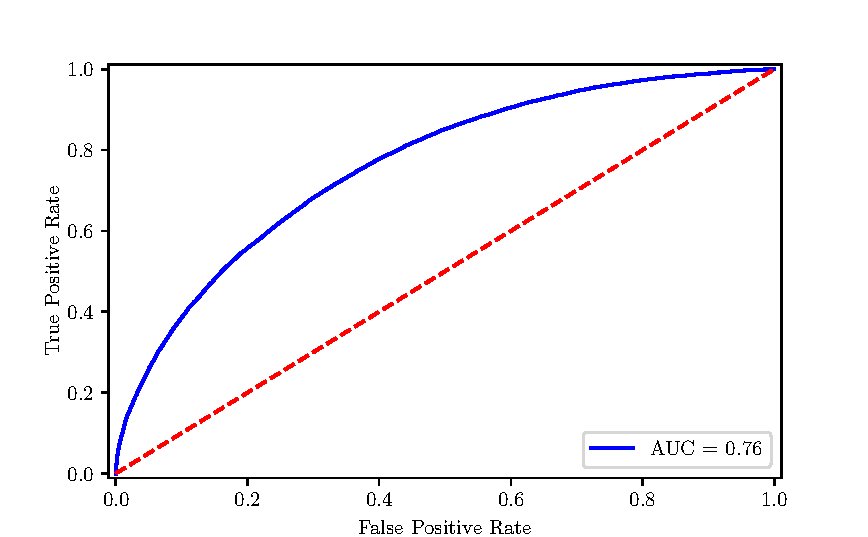
\includegraphics[width=\linewidth,height=.2\textheight,keepaspectratio]{readmitted30d/readmitted30d_ROC.pdf}
    \includegraphics[width=\linewidth,height=.2\textheight,keepaspectratio]{\picdir\picroc}
    % \input{test2.pgf} %% pgf not working for some reason
\end{subfigure}
\begin{subfigure}[t]{.45\linewidth}
    \centering
    \captionsetup[subfigure]{}
    \caption{Calibration curve.}\label{fig:cal30d}
    \includegraphics[width=\linewidth,height=.2\textheight,keepaspectratio]{\picdir\piccal}
    \vspace{2.5mm}
\end{subfigure}

\begin{subfigure}[t]{.45\linewidth}
    \vspace{2.5mm}
    \centering
    \captionsetup[subfigure]{}
    \caption{Bar summary of most impactful features.}\label{fig:shapsumbar30d}
    \includegraphics[width=\linewidth,height=.40\textheight,keepaspectratio]{\picdir\picbar}
    % \vspace{2.5mm}
\end{subfigure}
\begin{subfigure}[t]{.45\linewidth}
    \vspace{2.5mm}
    \centering
    \captionsetup[subfigure]{}
    \caption{Summary of most impactful features.}\label{fig:shapsum30d}
    \vspace{-2.3mm}
    \includegraphics[width=\linewidth,height=.38\textheight,keepaspectratio]{\picdir\picsum}
    \vspace{2.0mm}
\end{subfigure}
\textsf{Individualized predictions with interpretation.}
\vspace{-2.5mm}
\begin{subfigure}[t]{0.1\textwidth}
    \caption{}\label{fig:shapforce30d1}
    \end{subfigure}%
    \begin{minipage}[c]{0.9\textwidth}
    \includegraphics[width=\linewidth,keepaspectratio]{\picdir\picfpone}
    \vspace{-2.5mm}
\end{minipage}
\begin{subfigure}[t]{0.1\textwidth}
    \caption{}\label{fig:shapforce30d2}
    \end{subfigure}%
    \begin{minipage}[c]{0.9\textwidth}
    \includegraphics[width=\linewidth,keepaspectratio]{\picdir\picfptwo}
    \vspace{-3.5mm}
\end{minipage}
\vspace{-4.5mm}
\begin{subfigure}[t]{0.1\textwidth}
    \caption{}\label{fig:shapforce30d3}
    \end{subfigure}%
    \begin{minipage}[c]{0.9\textwidth}
    \includegraphics[width=\linewidth,keepaspectratio]{\picdir\picfpthr}
    \vspace{-2.5mm}
\end{minipage}
\vspace{-2.5mm}

\caption{\textbf{30-day Readmission.} \\\\
Model performance curves are shown for binary classification (Panel~\ref{fig:roc30d}) and probability calibration (Panel~\ref{fig:cal30d}).
Panels~\ref{fig:shapsumbar30d} and~\ref{fig:shapsum30d} show the most impactful features on prediction, 
along with the impact of high or low values for numeric features.\\\\
Panels~\ref{fig:shapforce30d1}--\ref{fig:shapforce30d3} show the composition of invididualized predictions for three patients.\@
The patient in~\ref{fig:shapforce30d1} was admitted from the emergency outpatient unit with a headache and stayed for over 7 days.\@
Additionally, they had been hospitalized 3 times prior to this admission, and had been discharged from their last admission only 8 days prior.\@
The model predicted their probability of 30-day readmission (0.30) was three times the baseline value predicted by the model (\textasciitilde0.1).\@
All of the listed features increased the model's prediction of risk by the relative amounts shown by the size of the red bars.\@
Conversely, the patient in~\ref{fig:shapforce30d3} was admitted for a complete uterovaginal prolapse, stayed less than a full day, and had
no reported comorbidities such as hypertension, depression, or a history of cancer.\@
The model predicted their probability of 30-day readmission at 0.3, or roughly one third of the baseline prediction.
}\label{fig:30dreadmission}
\end{adjustbox}
\end{figure}%

\onecolumn{}
\begin{figure}
\begin{adjustbox}{minipage={\linewidth},frame}
\vspace{2.5mm}
\centering

\def\picdir{los5d/}
\def\picroc{los5d_ROC.pdf}
\def\piccal{los5d_cal.pdf}
\def\picbar{los5d_SHAP_summary_bar.pdf}
\def\picsum{los5d_SHAP_summary.pdf}
\def\picfpone{los5d_10_SHAP_Pt_5529.png}
\def\picfptwo{los5d_10_SHAP_Pt_1434c2.png}
\def\picfpthr{los5d_10_SHAP_Pt_11022c2.png}

\begin{subfigure}[t]{.45\linewidth}
    \centering
    \captionsetup[subfigure]{}
    \caption[t]{Receiver operator characteristic curve.}\label{fig:roclos5d}
    % 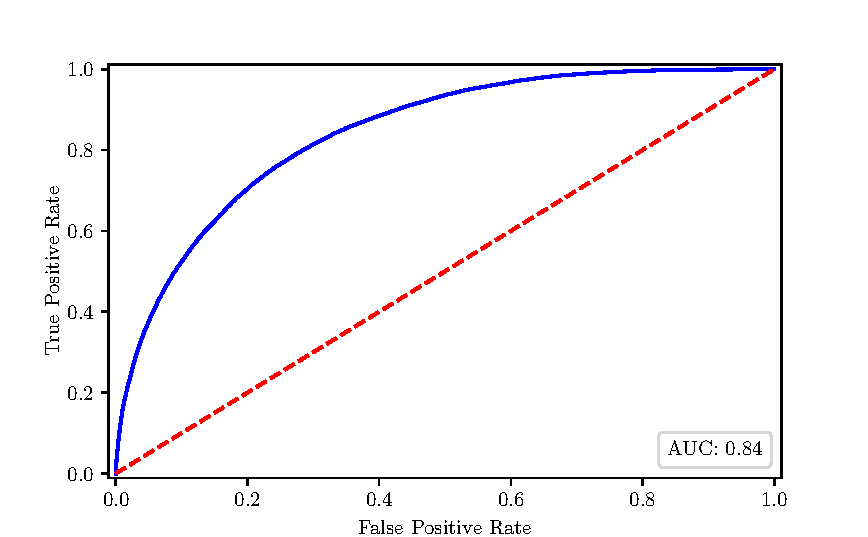
\includegraphics[width=\linewidth,height=.2\textheight,keepaspectratio]{los5d/los5d_ROC.pdf}
    \includegraphics[width=\linewidth,height=.2\textheight,keepaspectratio]{\picdir\picroc}
    % \input{test2.pgf} %% pgf not working for some reason
\end{subfigure}
\begin{subfigure}[t]{.45\linewidth}
    \centering
    \captionsetup[subfigure]{}
    \caption{Calibration curve.}\label{fig:callos5d}
    \includegraphics[width=\linewidth,height=.2\textheight,keepaspectratio]{\picdir\piccal}
    \vspace{2.5mm}
\end{subfigure}

\begin{subfigure}[t]{.45\linewidth}
    \vspace{2.5mm}
    \centering
    \captionsetup[subfigure]{}
    \caption{Bar summary of most impactful features.}\label{fig:shapsumbarlos5d}
    \includegraphics[width=\linewidth,height=.40\textheight,keepaspectratio]{\picdir\picbar}
    % \vspace{2.5mm}
\end{subfigure}
\begin{subfigure}[t]{.45\linewidth}
    \vspace{2.5mm}
    \centering
    \captionsetup[subfigure]{}
    \caption{Summary of most impactful features.}\label{fig:shapsumlos5d}
    \vspace{-2.3mm}
    \includegraphics[width=\linewidth,height=.38\textheight,keepaspectratio]{\picdir\picsum}
    \vspace{2.0mm}
\end{subfigure}
\textsf{Individualized predictions with interpretation.}
\vspace{-2.5mm}
\begin{subfigure}[t]{0.1\textwidth}
    \caption{}\label{fig:shapforcelos5d1}
    \end{subfigure}%
    \begin{minipage}[c]{0.9\textwidth}
    \includegraphics[width=\linewidth,keepaspectratio]{\picdir\picfpone}
    \vspace{-2.5mm}
\end{minipage}
\begin{subfigure}[t]{0.1\textwidth}
    \caption{}\label{fig:shapforcelos5d2}
    \end{subfigure}%
    \begin{minipage}[c]{0.9\textwidth}
    \includegraphics[width=\linewidth,keepaspectratio]{\picdir\picfptwo}
    \vspace{-3.5mm}
\end{minipage}
\vspace{-4.5mm}
\begin{subfigure}[t]{0.1\textwidth}
    \caption{}\label{fig:shapforcelos5d3}
    \end{subfigure}%
    \begin{minipage}[c]{0.9\textwidth}
    \includegraphics[width=\linewidth,keepaspectratio]{\picdir\picfpthr}
    \vspace{-2.5mm}
\end{minipage}
\vspace{-2.5mm}

\caption{\textbf{Length of Stay Over 5 Days.} \\\\
Model performance curves are shown for binary classification (Panel~\ref{fig:roclos5d}) and probability calibration (Panel~\ref{fig:callos5d}).\\\\
Panels~\ref{fig:shapsumbarlos5d} and~\ref{fig:shapsumlos5d} shows the most impactful features on prediction, 
along with the impact of high or low values for numeric features.%
For~\ref{fig:shapsumlos5d}, the line is made of individual dots representing each admission,
and the thickness of the line is determined by the number of examples at a given value (for example, many of our patients are elderly).
A negative SHAP value explains a reduced probability, while a positive one increases it.
For example, advanced age increases the probability of extended length of stay (SHAP value between zero and one), 
while young age tends toward a SHAP value between roughly -1 and zero, corresponding to reduced probability.
For non-numeric features, such as primary diagnosis, the gray points represent specific possible values, with certain diagnoses greatly
increasing or reducing the model's output, while the majority of diagnoses have relatively mild impact on prediction.\\\\
Panels~\ref{fig:shapforcelos5d1}--\ref{fig:shapforcelos5d3} show the composition of invididualized predictions for three patients.
The 75-year-old patient in~\ref{fig:shapforcelos5d1} was admitted to the inpatient service directly from an MD's office with leakage of a heart valve graft.
The patient received 32 medications in the first 24 hours, and has Medicare Part A insurance coverage.
The model predicted the patient's probability of staying longer than five days was 0.80, 
nearly four times the baseline prediction of \textasciitilde0.2.
The majority of the model's prediction was based on the diagnosis, followed by the number of initial medications, and then the other variables as shown.
The patient in~\ref{fig:shapforcelos5d3}, on the other hand, had a predicted probability of length of stay of 0.06, 
or roughly one fourth of the baseline, despite being admitted to the ICU within 24 hours of admission.
The major contributor to this low probability was the diagnosis of antidepressant poisoning, followed by insurance provider,
and, finally, by a lack of BMI recorded in the chart for this encounter.
}\label{fig:los5d}
\end{adjustbox}
\end{figure}%

\pagestyle{fancy}
\onecolumn{}
\begin{figure}
\begin{adjustbox}{minipage=7.0in,frame}
% \begin{adjustbox}{width=7in,totalheight=7in,frame}
\vspace{2.5mm}
\centering

% \hspace{5mm}%
\begin{subfigure}[t]{.45\linewidth}
    \centering
    \captionsetup[subfigure]{}
    \caption{Gender.}\label{fig:shapsumgender}
    % 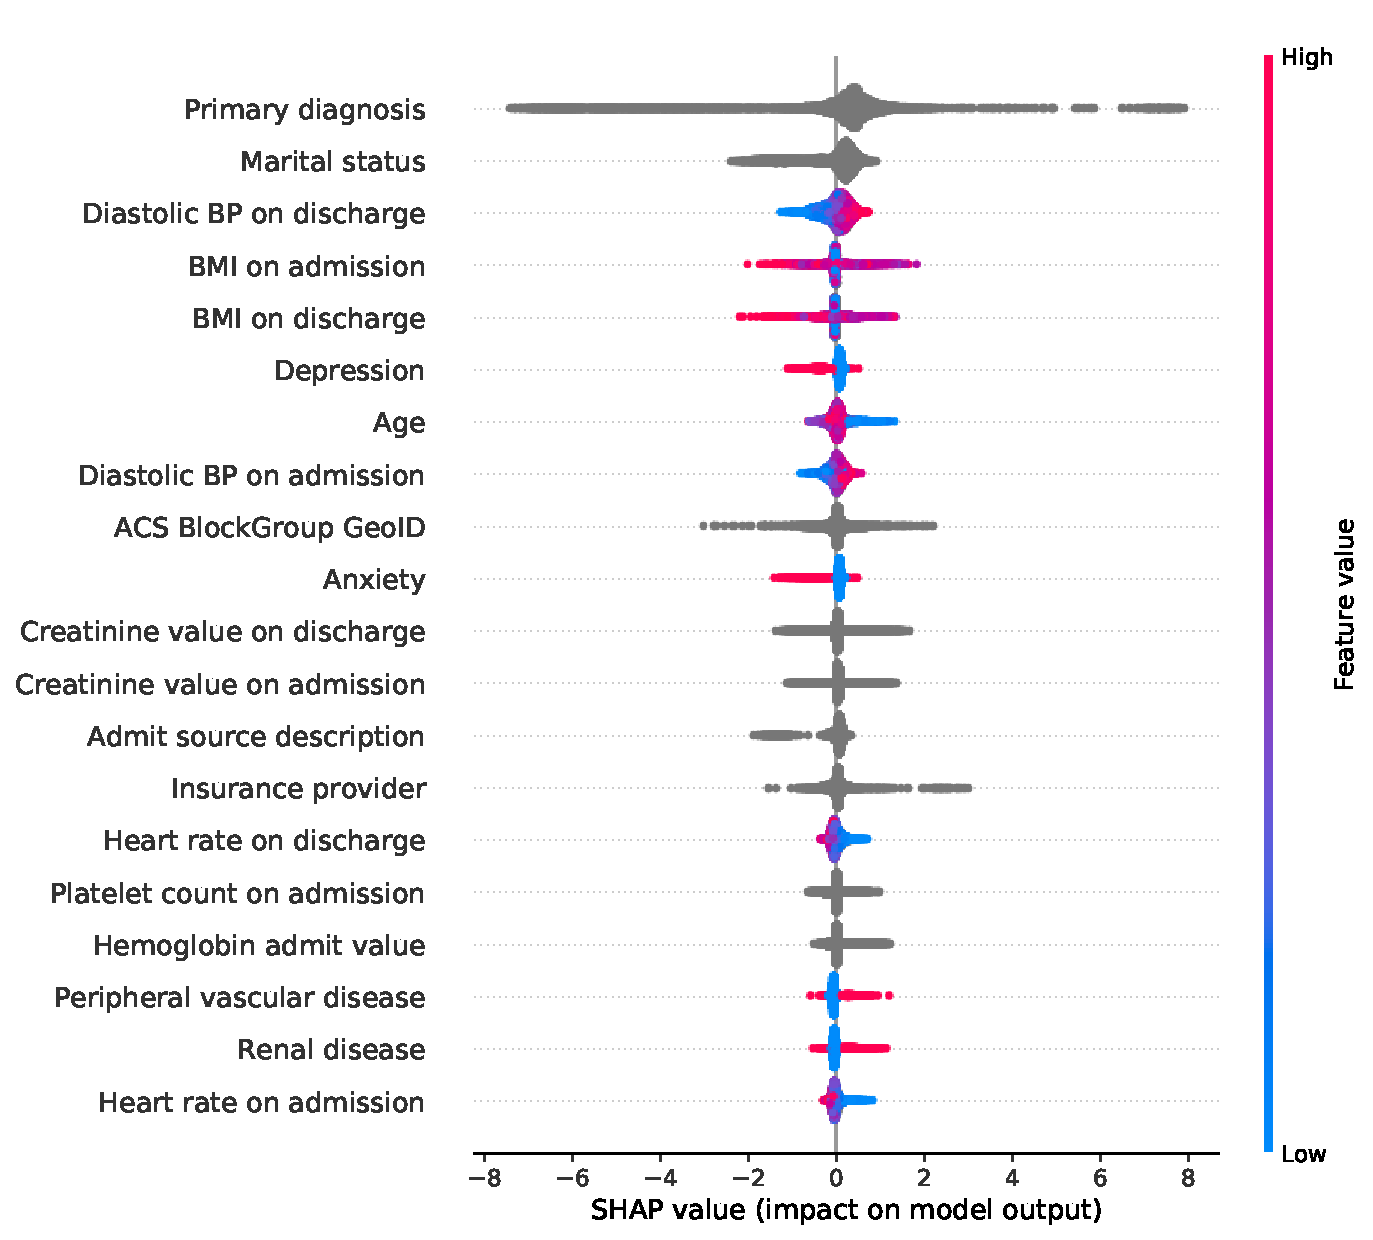
\includegraphics[width=\linewidth,keepaspectratio]{other/gender_SHAP_summary.pdf}
    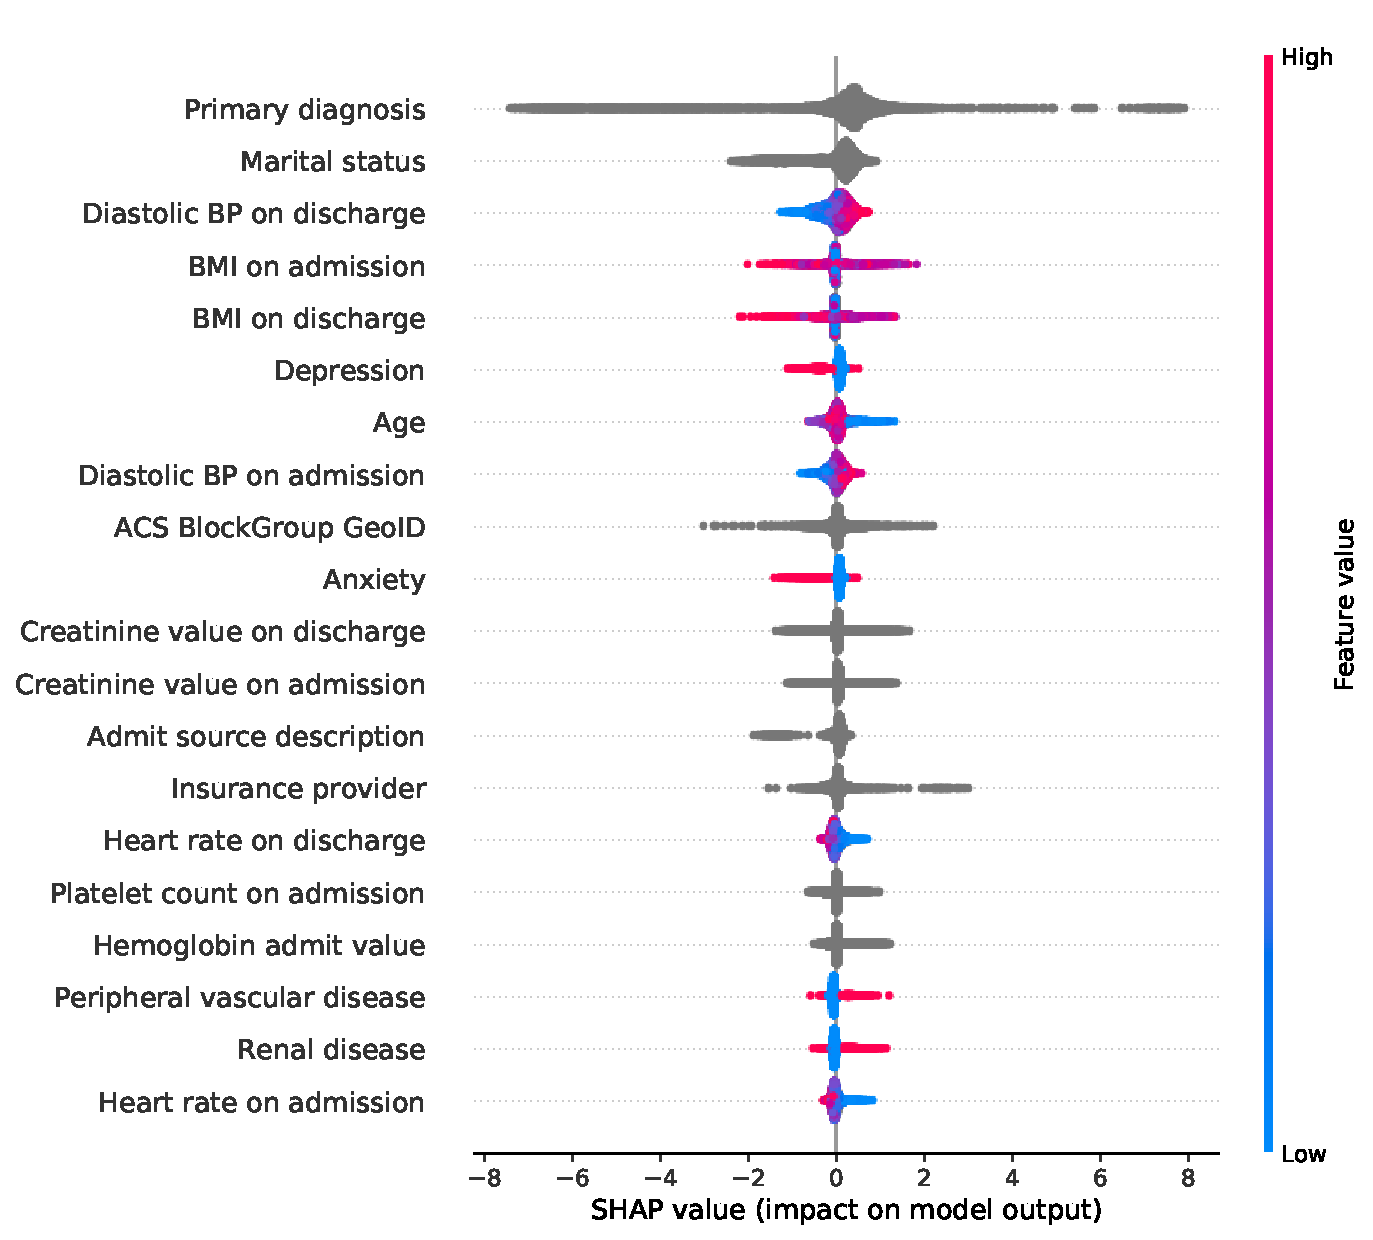
\includegraphics[height=3in,width=3in]{other/gender_SHAP_summary.pdf}
\end{subfigure}%
\hspace{5mm}%
\begin{subfigure}[t]{.45\linewidth}
    \centering
    \captionsetup[subfigure]{}
    \caption{Age.}\label{fig:shapsumage}
    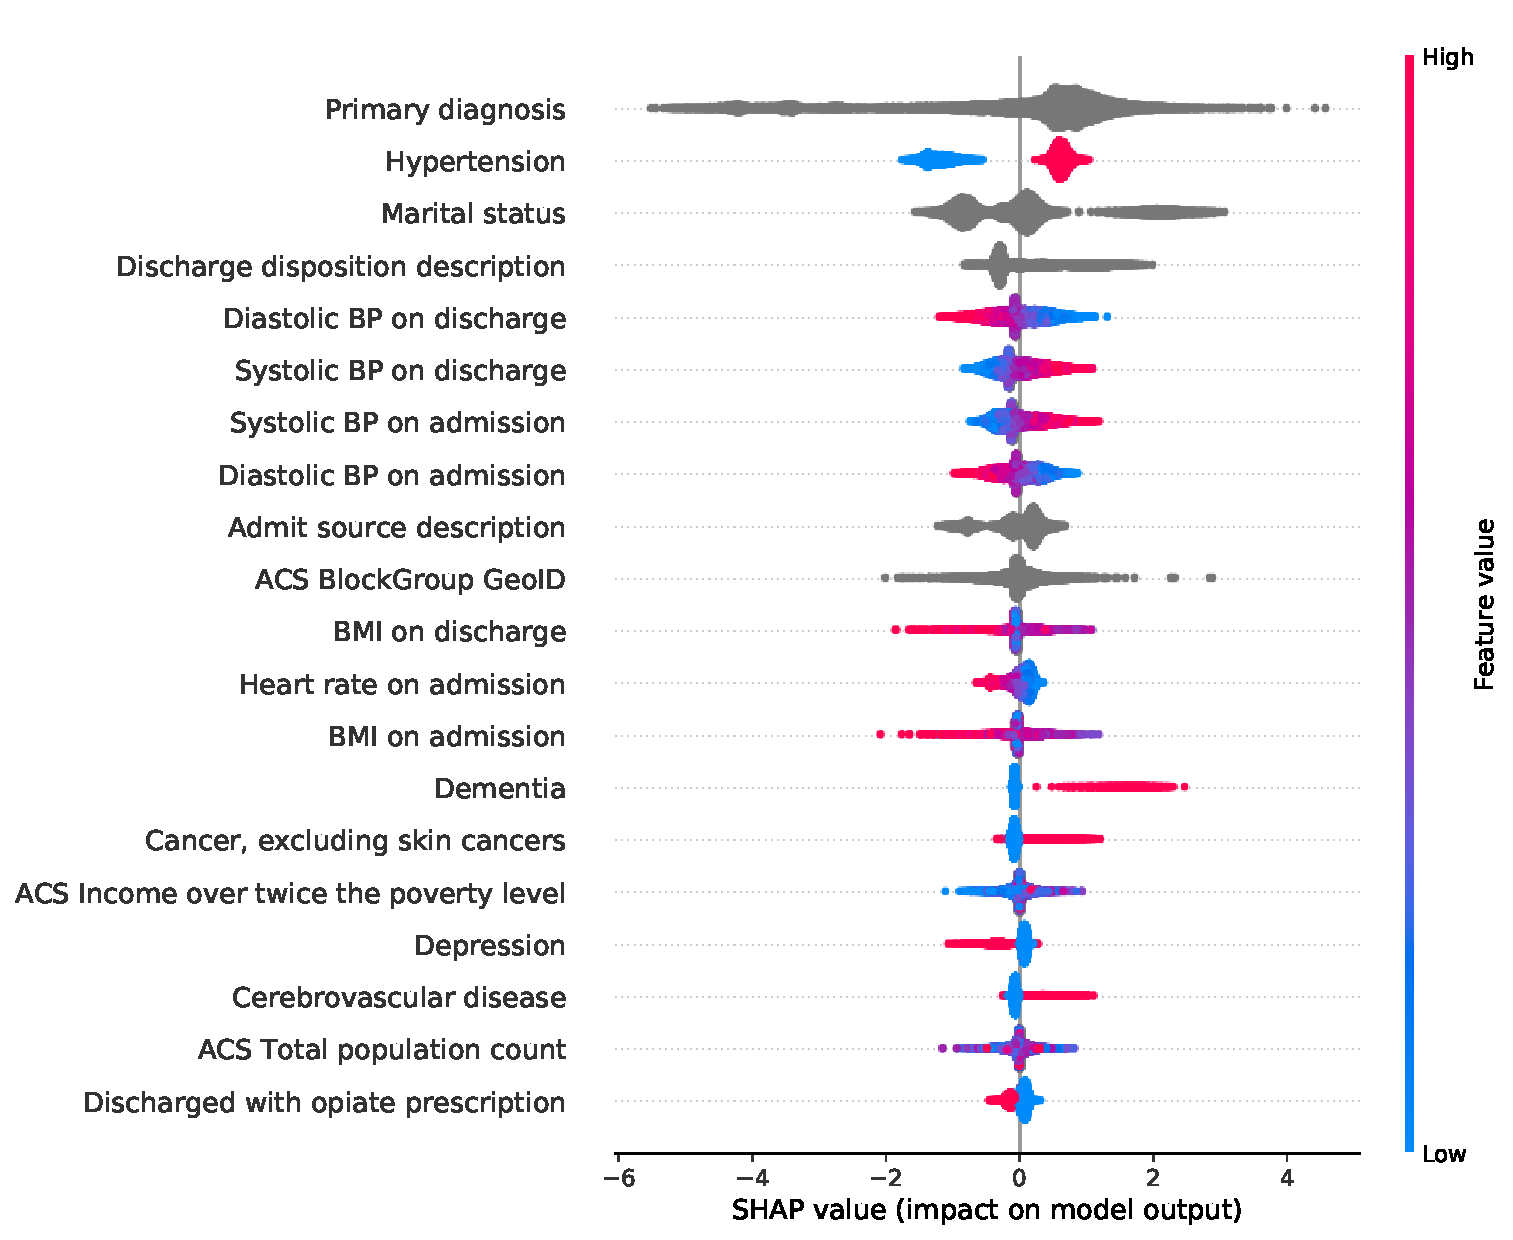
\includegraphics[height=3in,width=3in]{other/age_SHAP_summary.pdf}
    % 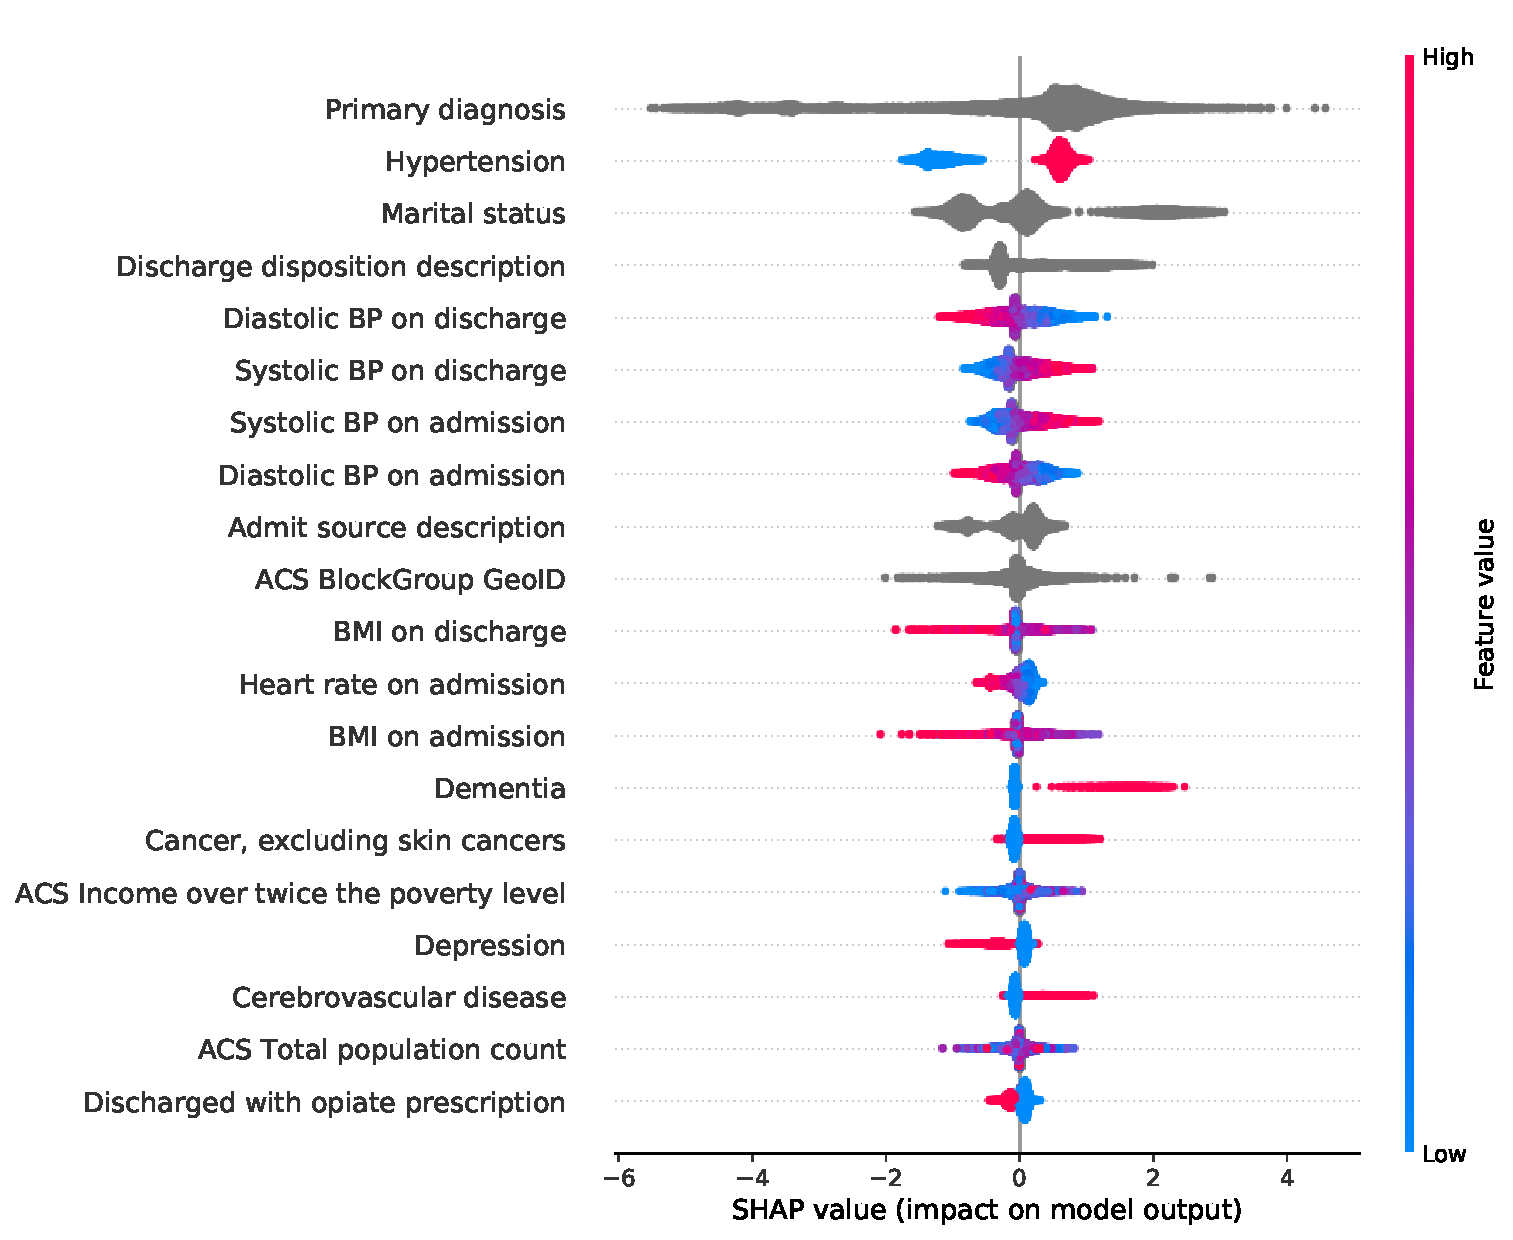
\includegraphics[width=\linewidth,keepaspectratio]{other/age_SHAP_summary.pdf}
\end{subfigure}%

\vspace{5mm}
% \hspace{5mm}%
\begin{subfigure}[t]{.45\linewidth}
    \centering
    \captionsetup[subfigure]{}
    \caption{Race. }\label{fig:shapsumrace}
    % \vspace{5mm}
    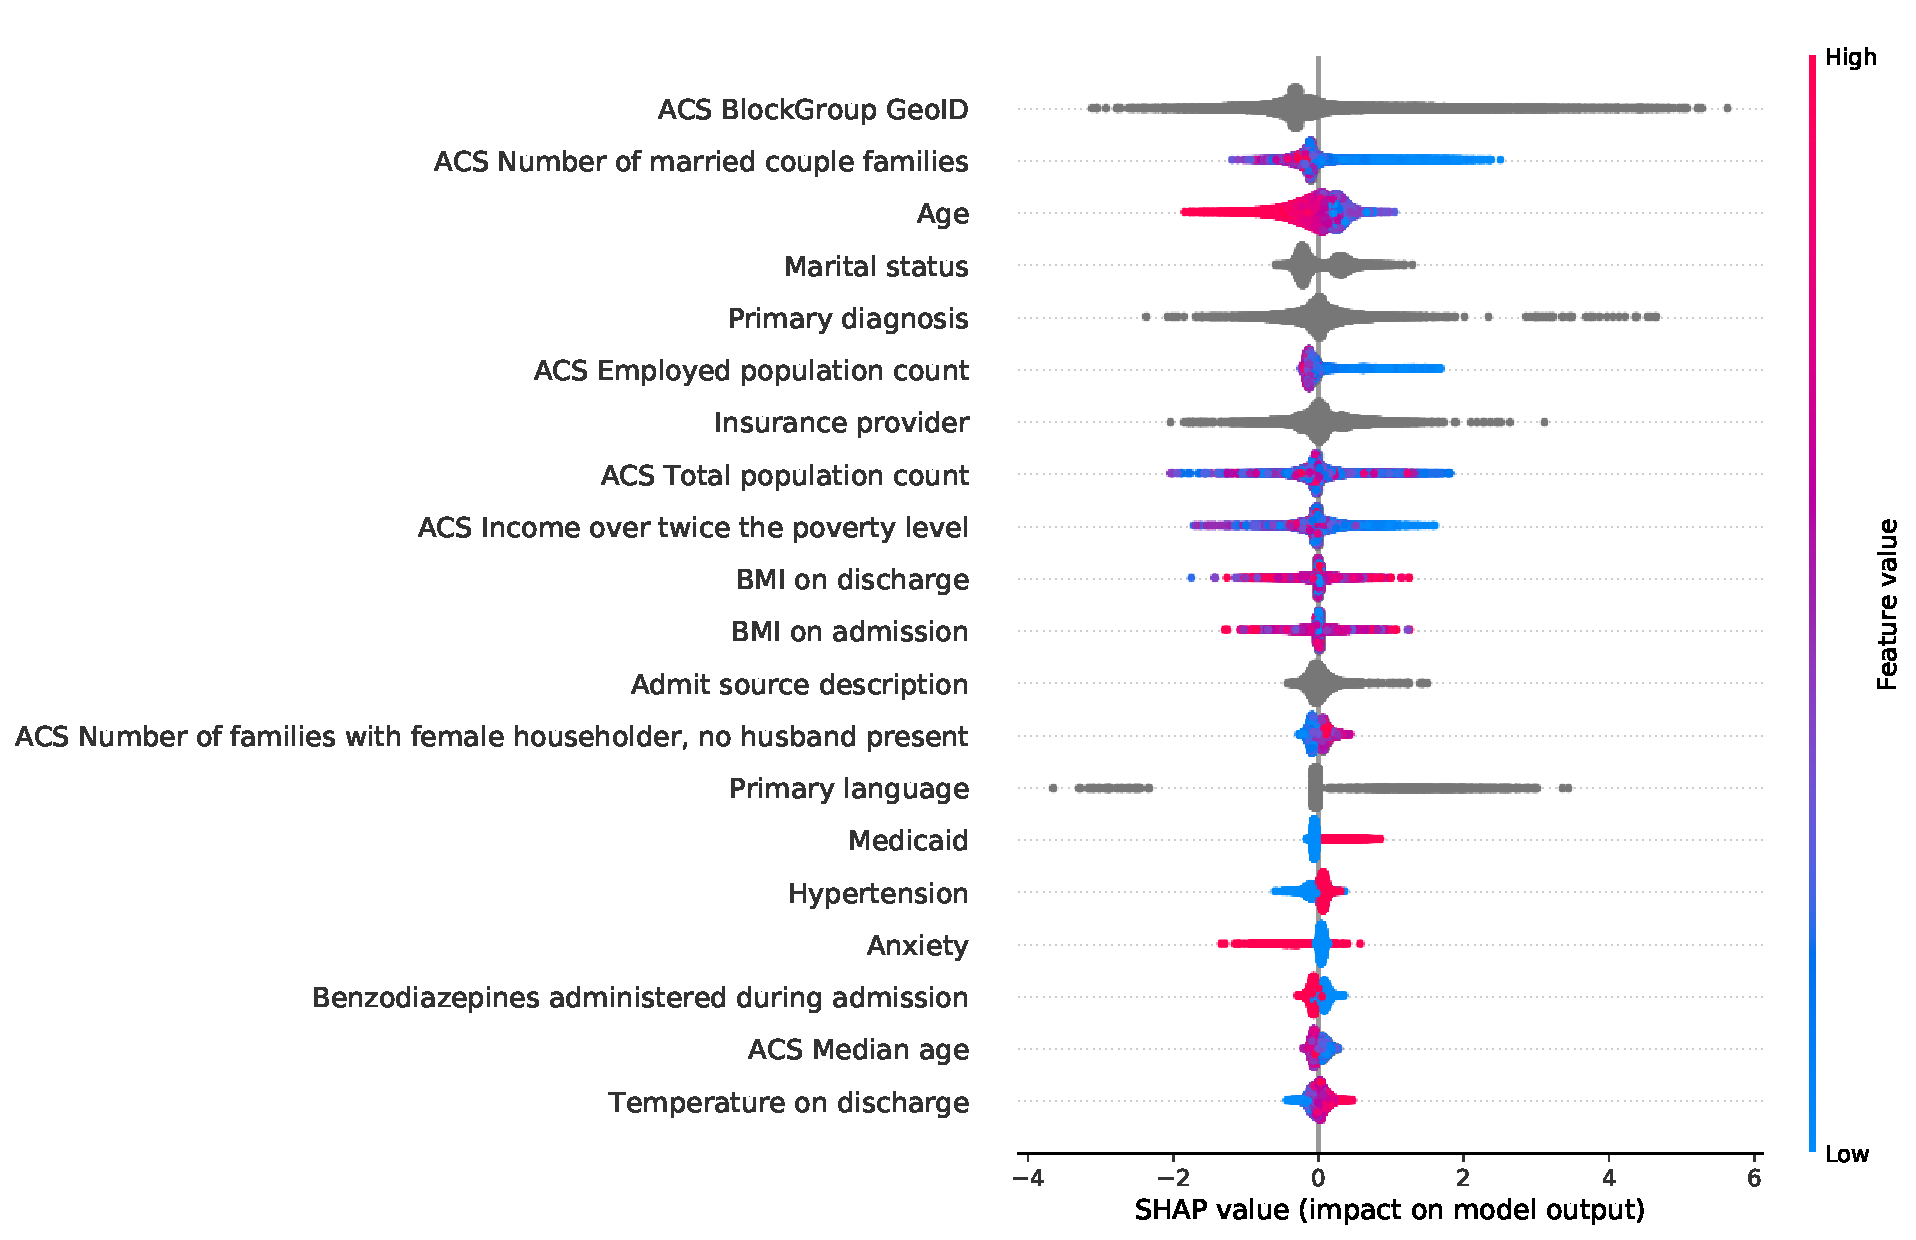
\includegraphics[height=2.7in,width=3in]{other/race_SHAP_summary.pdf}
    % \def\svgwidth{width=3in} %C:\Users\hiltonc\Desktop\readmit\reports\text\figdir\other\race_SHAP_summary_test.pdf_tex
    % \subimport{/other/}{race_SHAP_summary_test.pdf_tex}
    % \input{race_SHAP_summary_test.pdf_tex}
    % 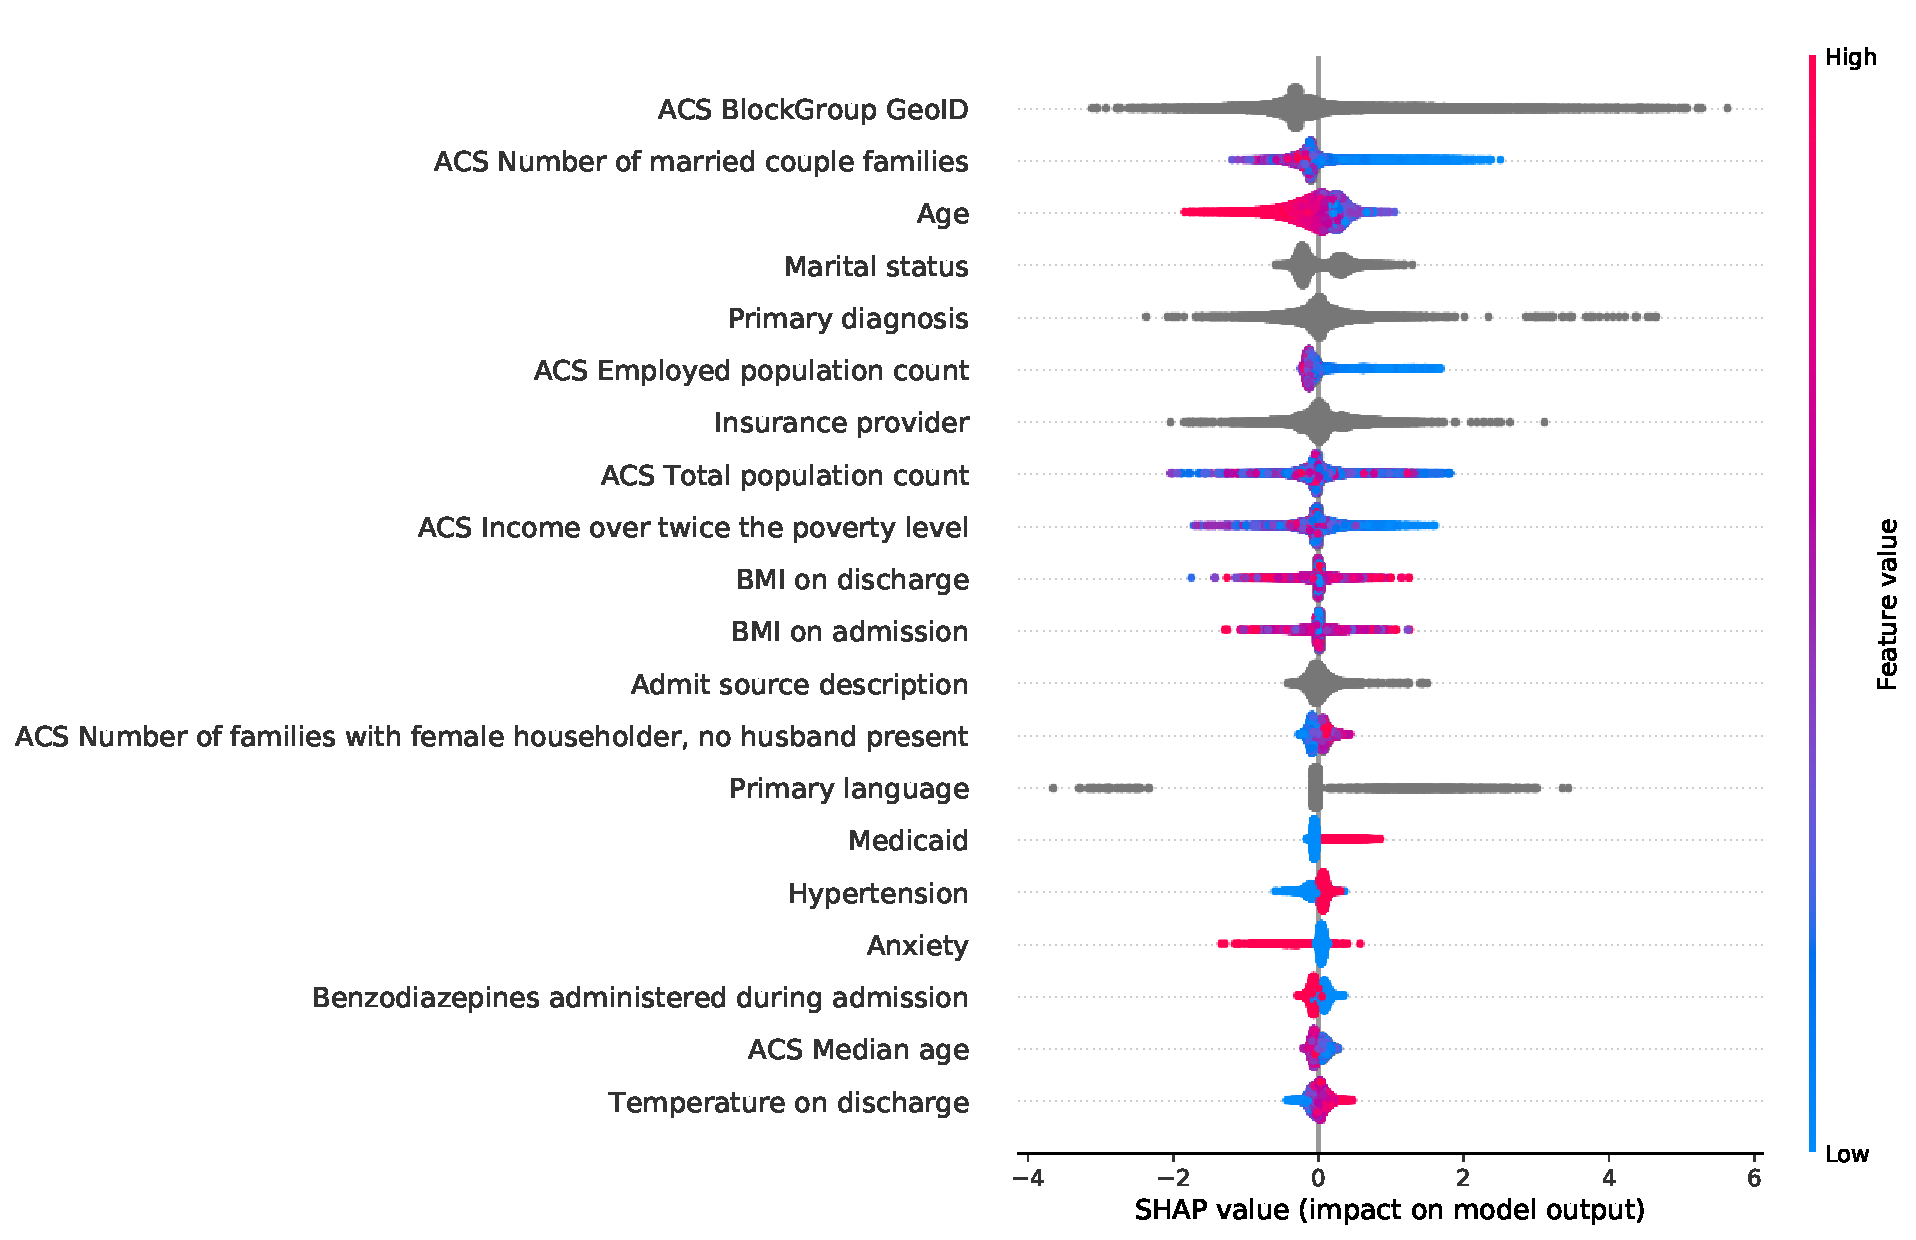
\includegraphics[width=\linewidth,keepaspectratio]{other/race_SHAP_summary.pdf}
\end{subfigure}%
\hspace{5mm}%
\begin{subfigure}[t]{.45\linewidth}
    \centering
    \captionsetup[subfigure]{}
    \caption{Payer class.}\label{fig:shapsuminsurance}
    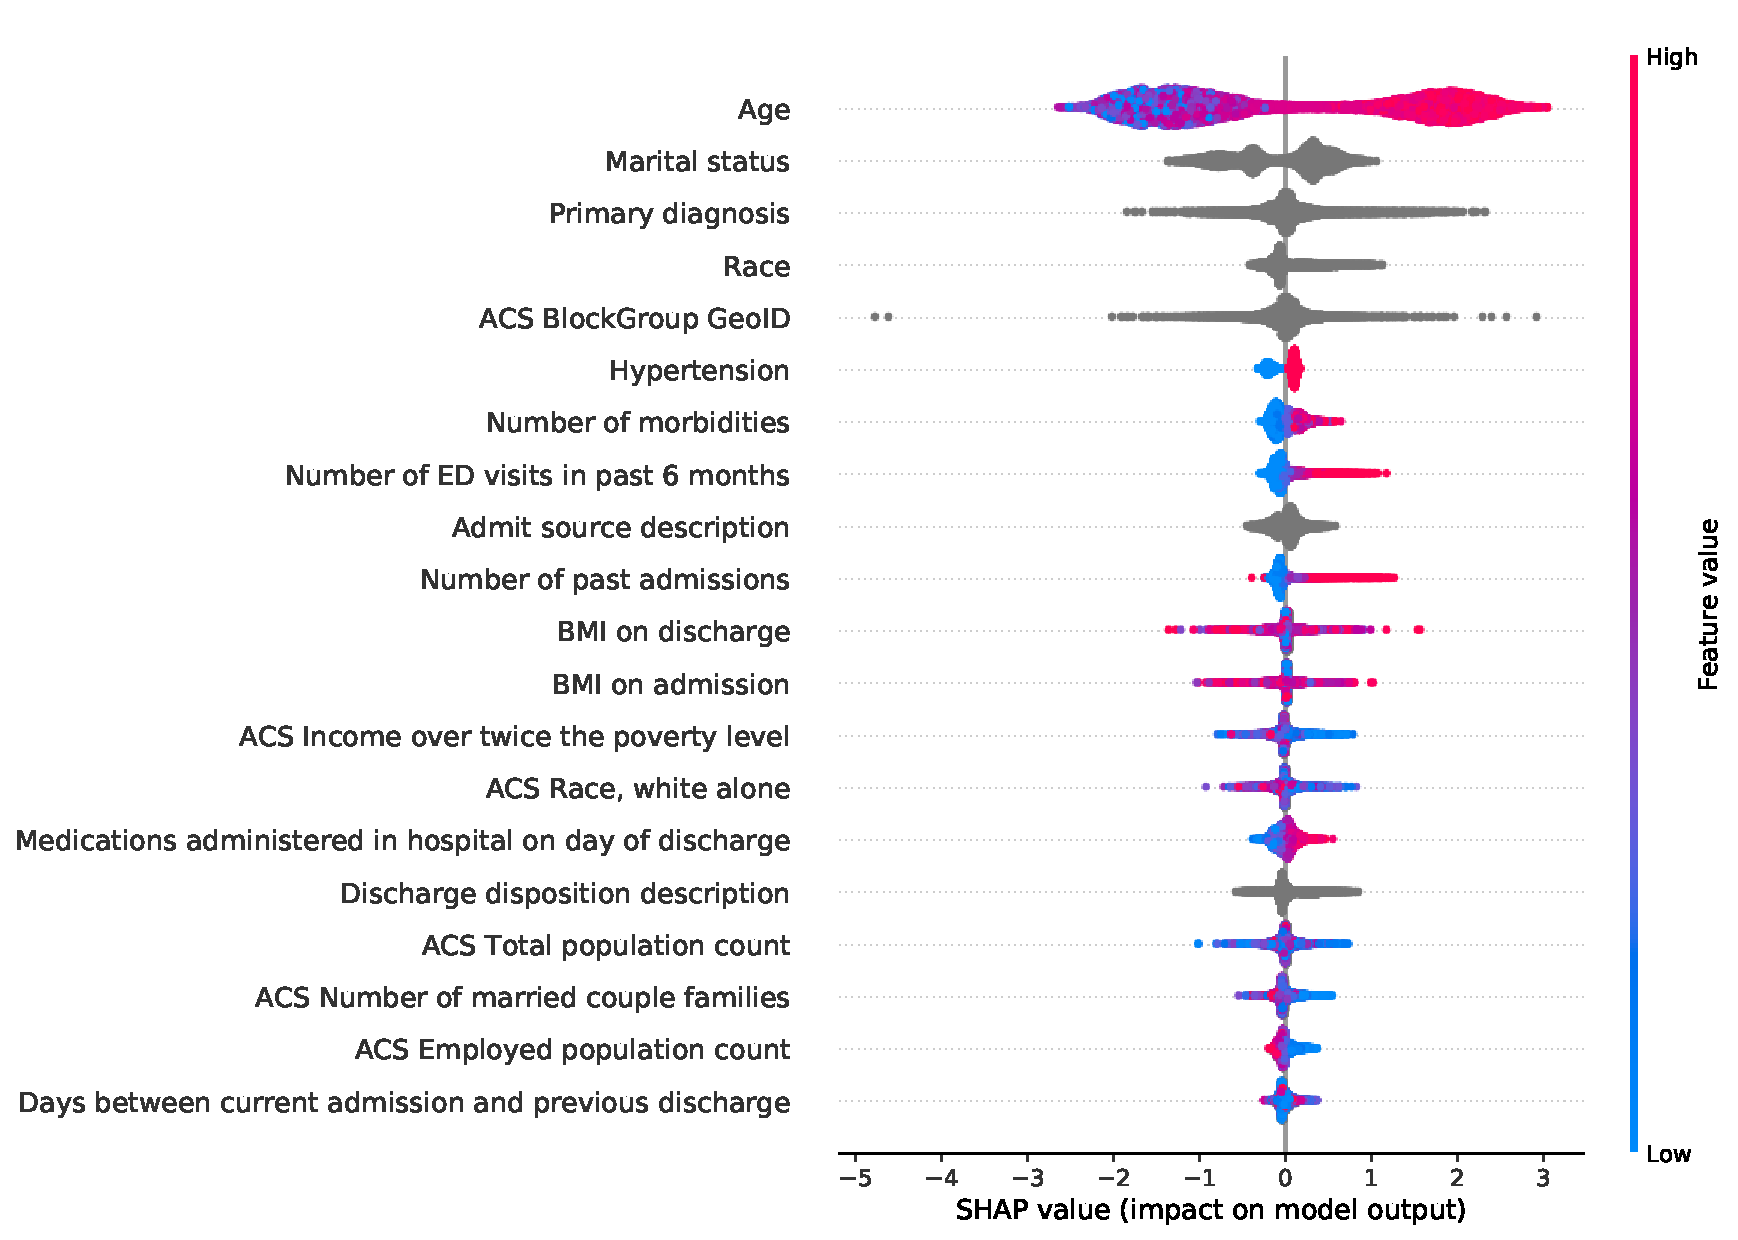
\includegraphics[height=2.7in,width=3in]{other/insurance_SHAP_summary.pdf}
    % 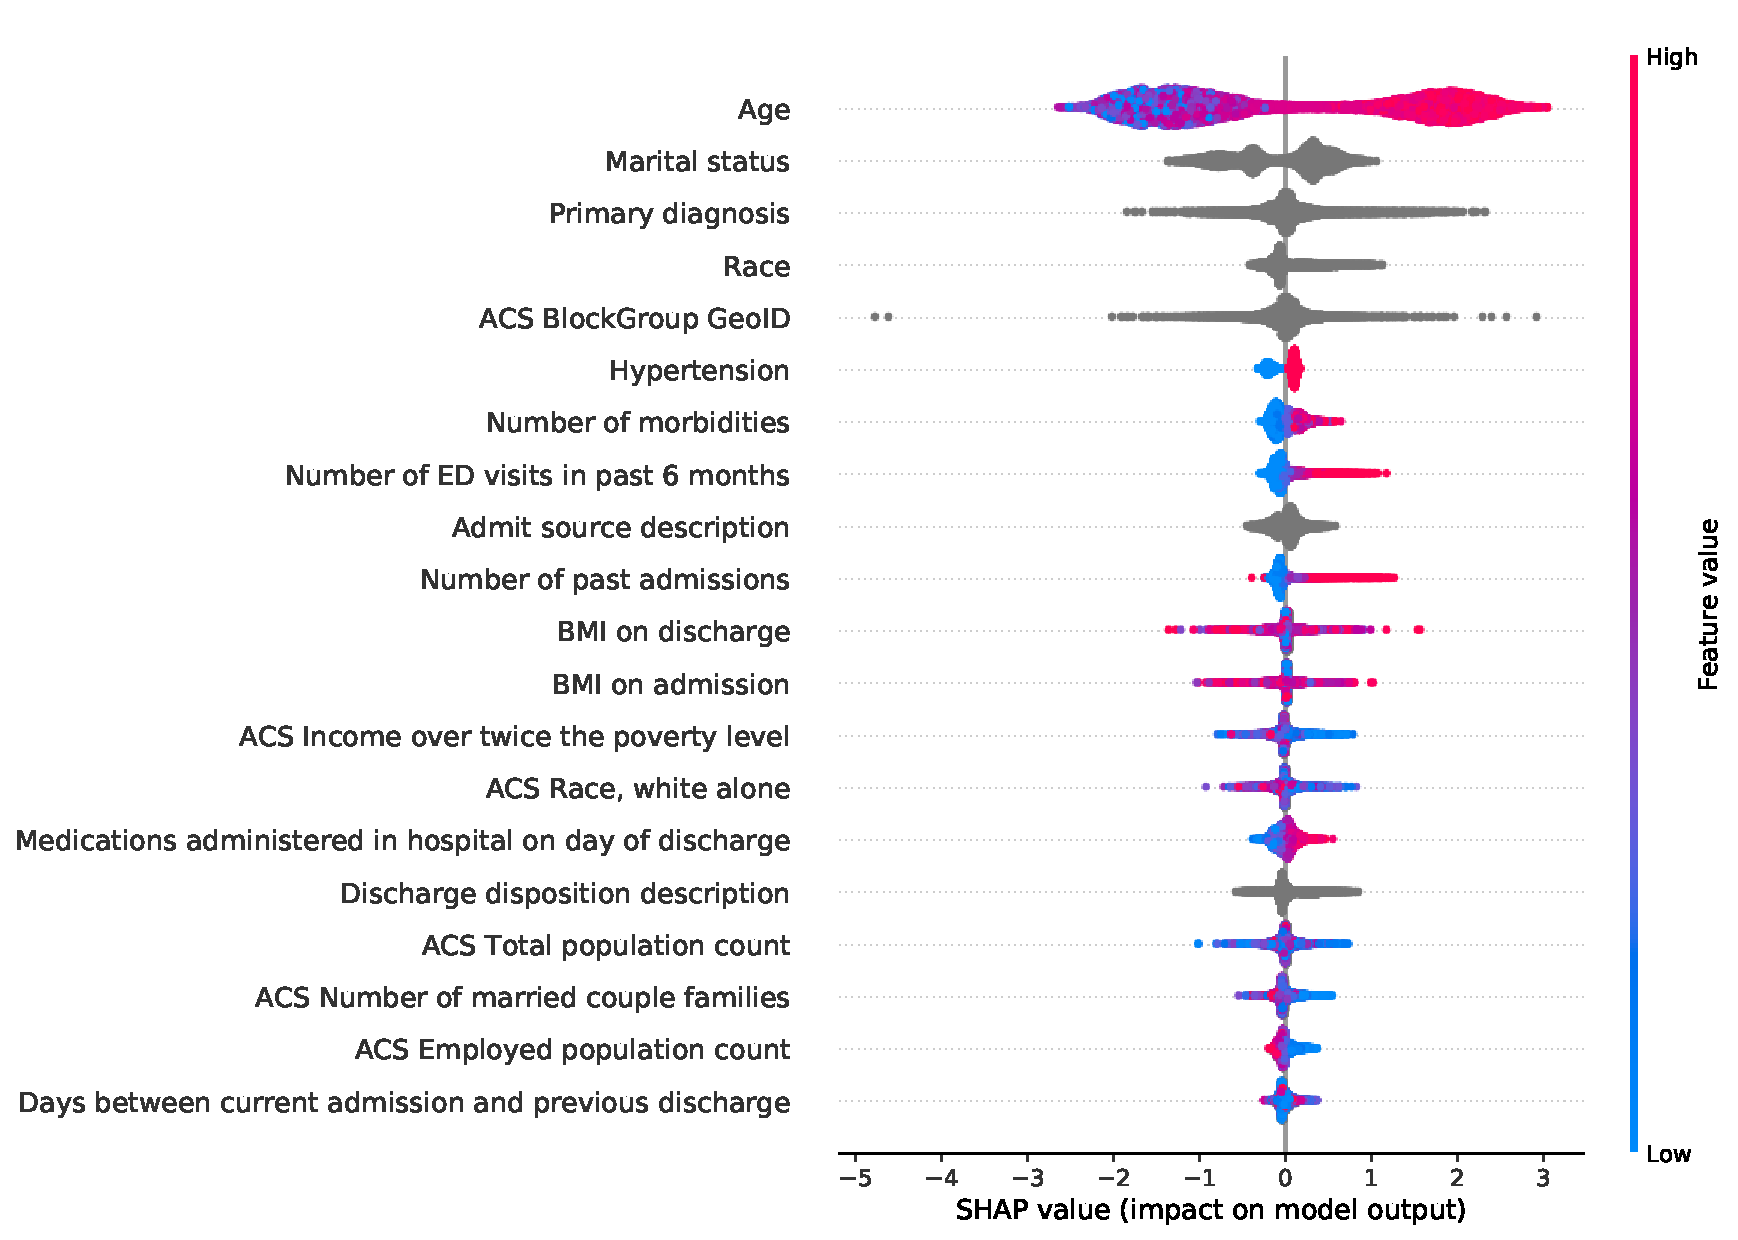
\includegraphics[width=\linewidth,keepaspectratio]{other/insurance_SHAP_summary.pdf}
\end{subfigure}%

% \noindent
% \rule[1ex]{width=\linewidth}{0.5pt}
\caption{\textbf{Prediction of Patient Characteristics.} \\
Panels~\ref{fig:shapsumgender},~\ref{fig:shapsumage},~\ref{fig:shapsumrace}, and~\ref{fig:shapsuminsurance} 
show the most impactful features on prediction, 
along with the impact of high or low values for numeric features. 
``ACS'' data is drawn from the American Community Survey for each patient's BlockGroup.
}\label{fig:otherfig}
\end{adjustbox}
\end{figure}
\clearpage
\pagestyle{fancy}%
% \noindent
% \rule[1ex]{width=\linewidth}{0.5pt}
% in{minipage}[t][0.5\textheight][t]{\textwidth} 





% \pagestyle{fancy}
% \onecolumn{}
% \begin{figure}
% \begin{adjustbox}{minipage=1.0\linewidth,frame}
% \vspace{2.5mm}
% \centering

% \begin{subfigure}[t]{.3\linewidth}
% % \centering
% \captionsetup[subfigure]{}
% \caption[t]{Receiver operator characteristic curve for gender.}\label{fig:rocgender}
% 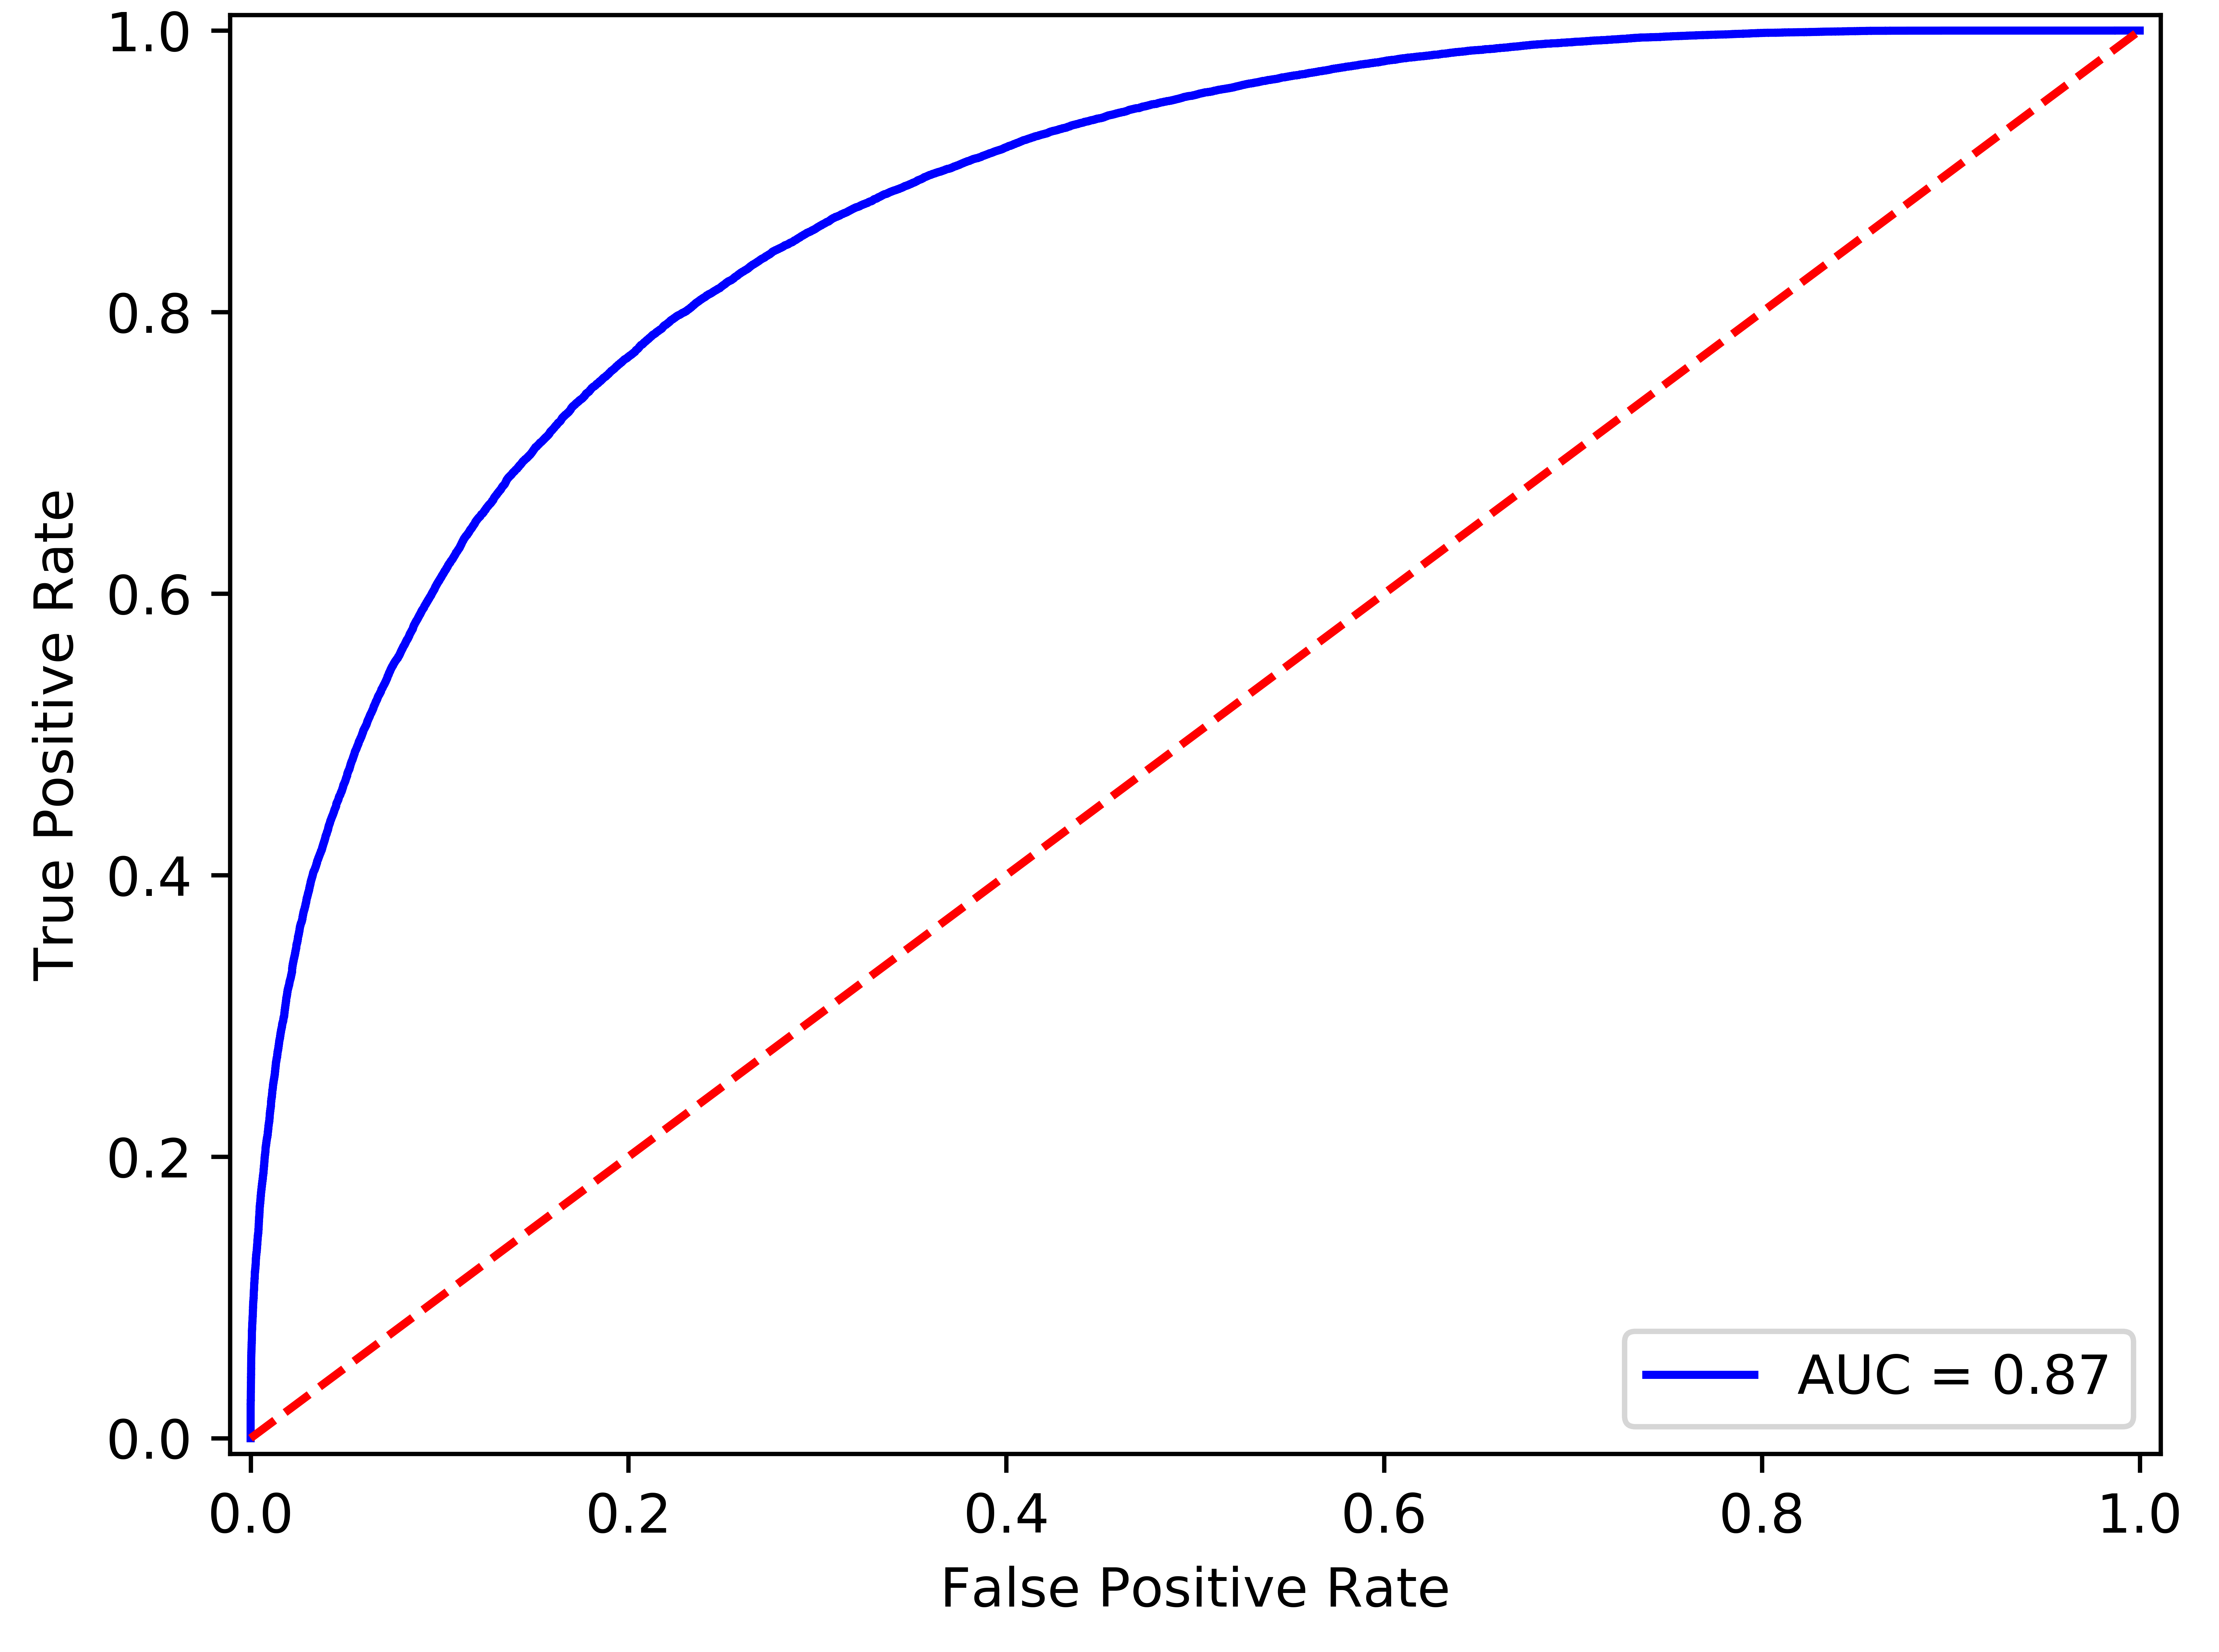
\includegraphics[width=\linewidth,height=.2\textheight,keepaspectratio]{other/gender_ROC.png}
% \end{subfigure}%
% \hspace{5mm}%
% \begin{subfigure}[t]{.5\linewidth}
%     \centering
%     \captionsetup[subfigure]{}
%     \caption{Summary of most impactful features for gender.}\label{fig:shapsumgender}
%     \includegraphics[width=\linewidth,keepaspectratio]{other/gender_SHAP_summary.png}
% \end{subfigure}%

% \begin{subfigure}[t]{.3\linewidth}
%     \centering
%     \captionsetup[subfigure]{}
%     \caption[t]{Receiver operator characteristic curve for race.}\label{fig:rocrace}
%     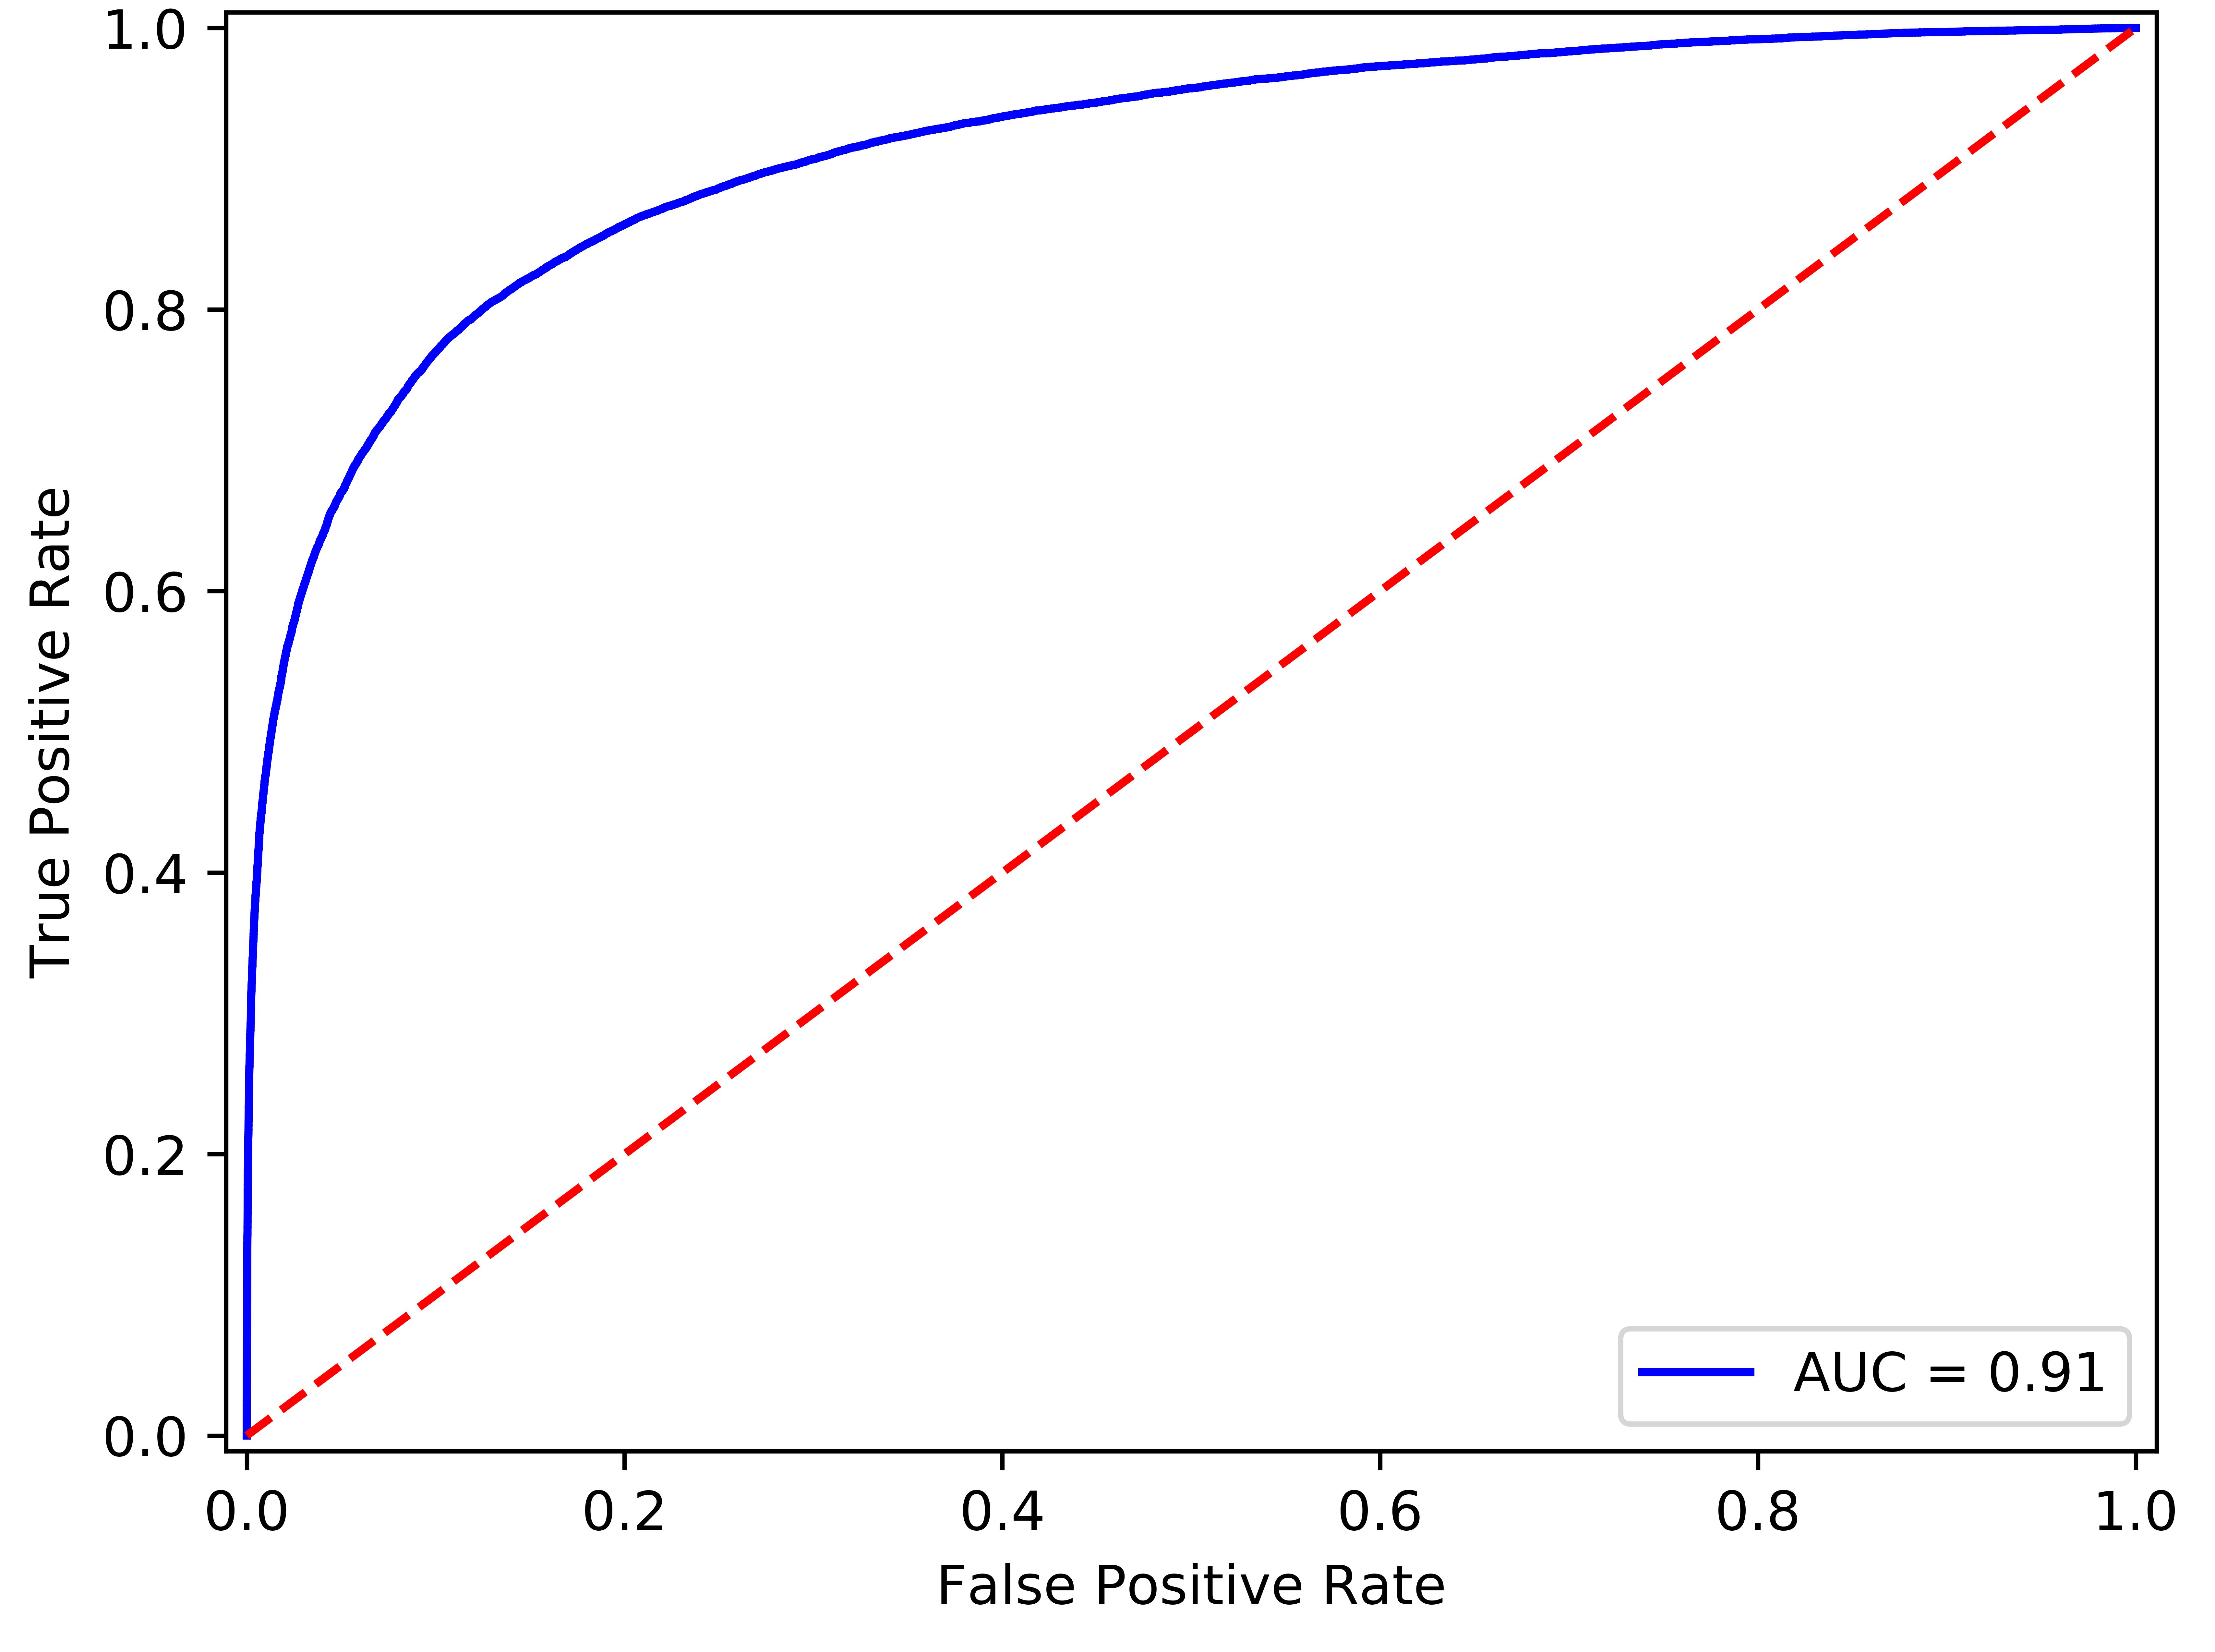
\includegraphics[width=\linewidth,height=.2\textheight,keepaspectratio]{other/race_ROC.png}
% \end{subfigure}%
% \hspace{5mm}%
% \begin{subfigure}[t]{.5\linewidth}
%     \centering
%     \captionsetup[subfigure]{}
%     \caption{Summary of most impactful features for race.}\label{fig:shapsumrace}
%     \includegraphics[width=\linewidth,keepaspectratio]{other/race_SHAP_summary.png}
% \end{subfigure}%

% \begin{subfigure}[t]{.3\linewidth}
%     \centering
%     \captionsetup[subfigure]{}
%     \caption[t]{Receiver operator characteristic curve for financial class.}\label{fig:rocinsurance}
%     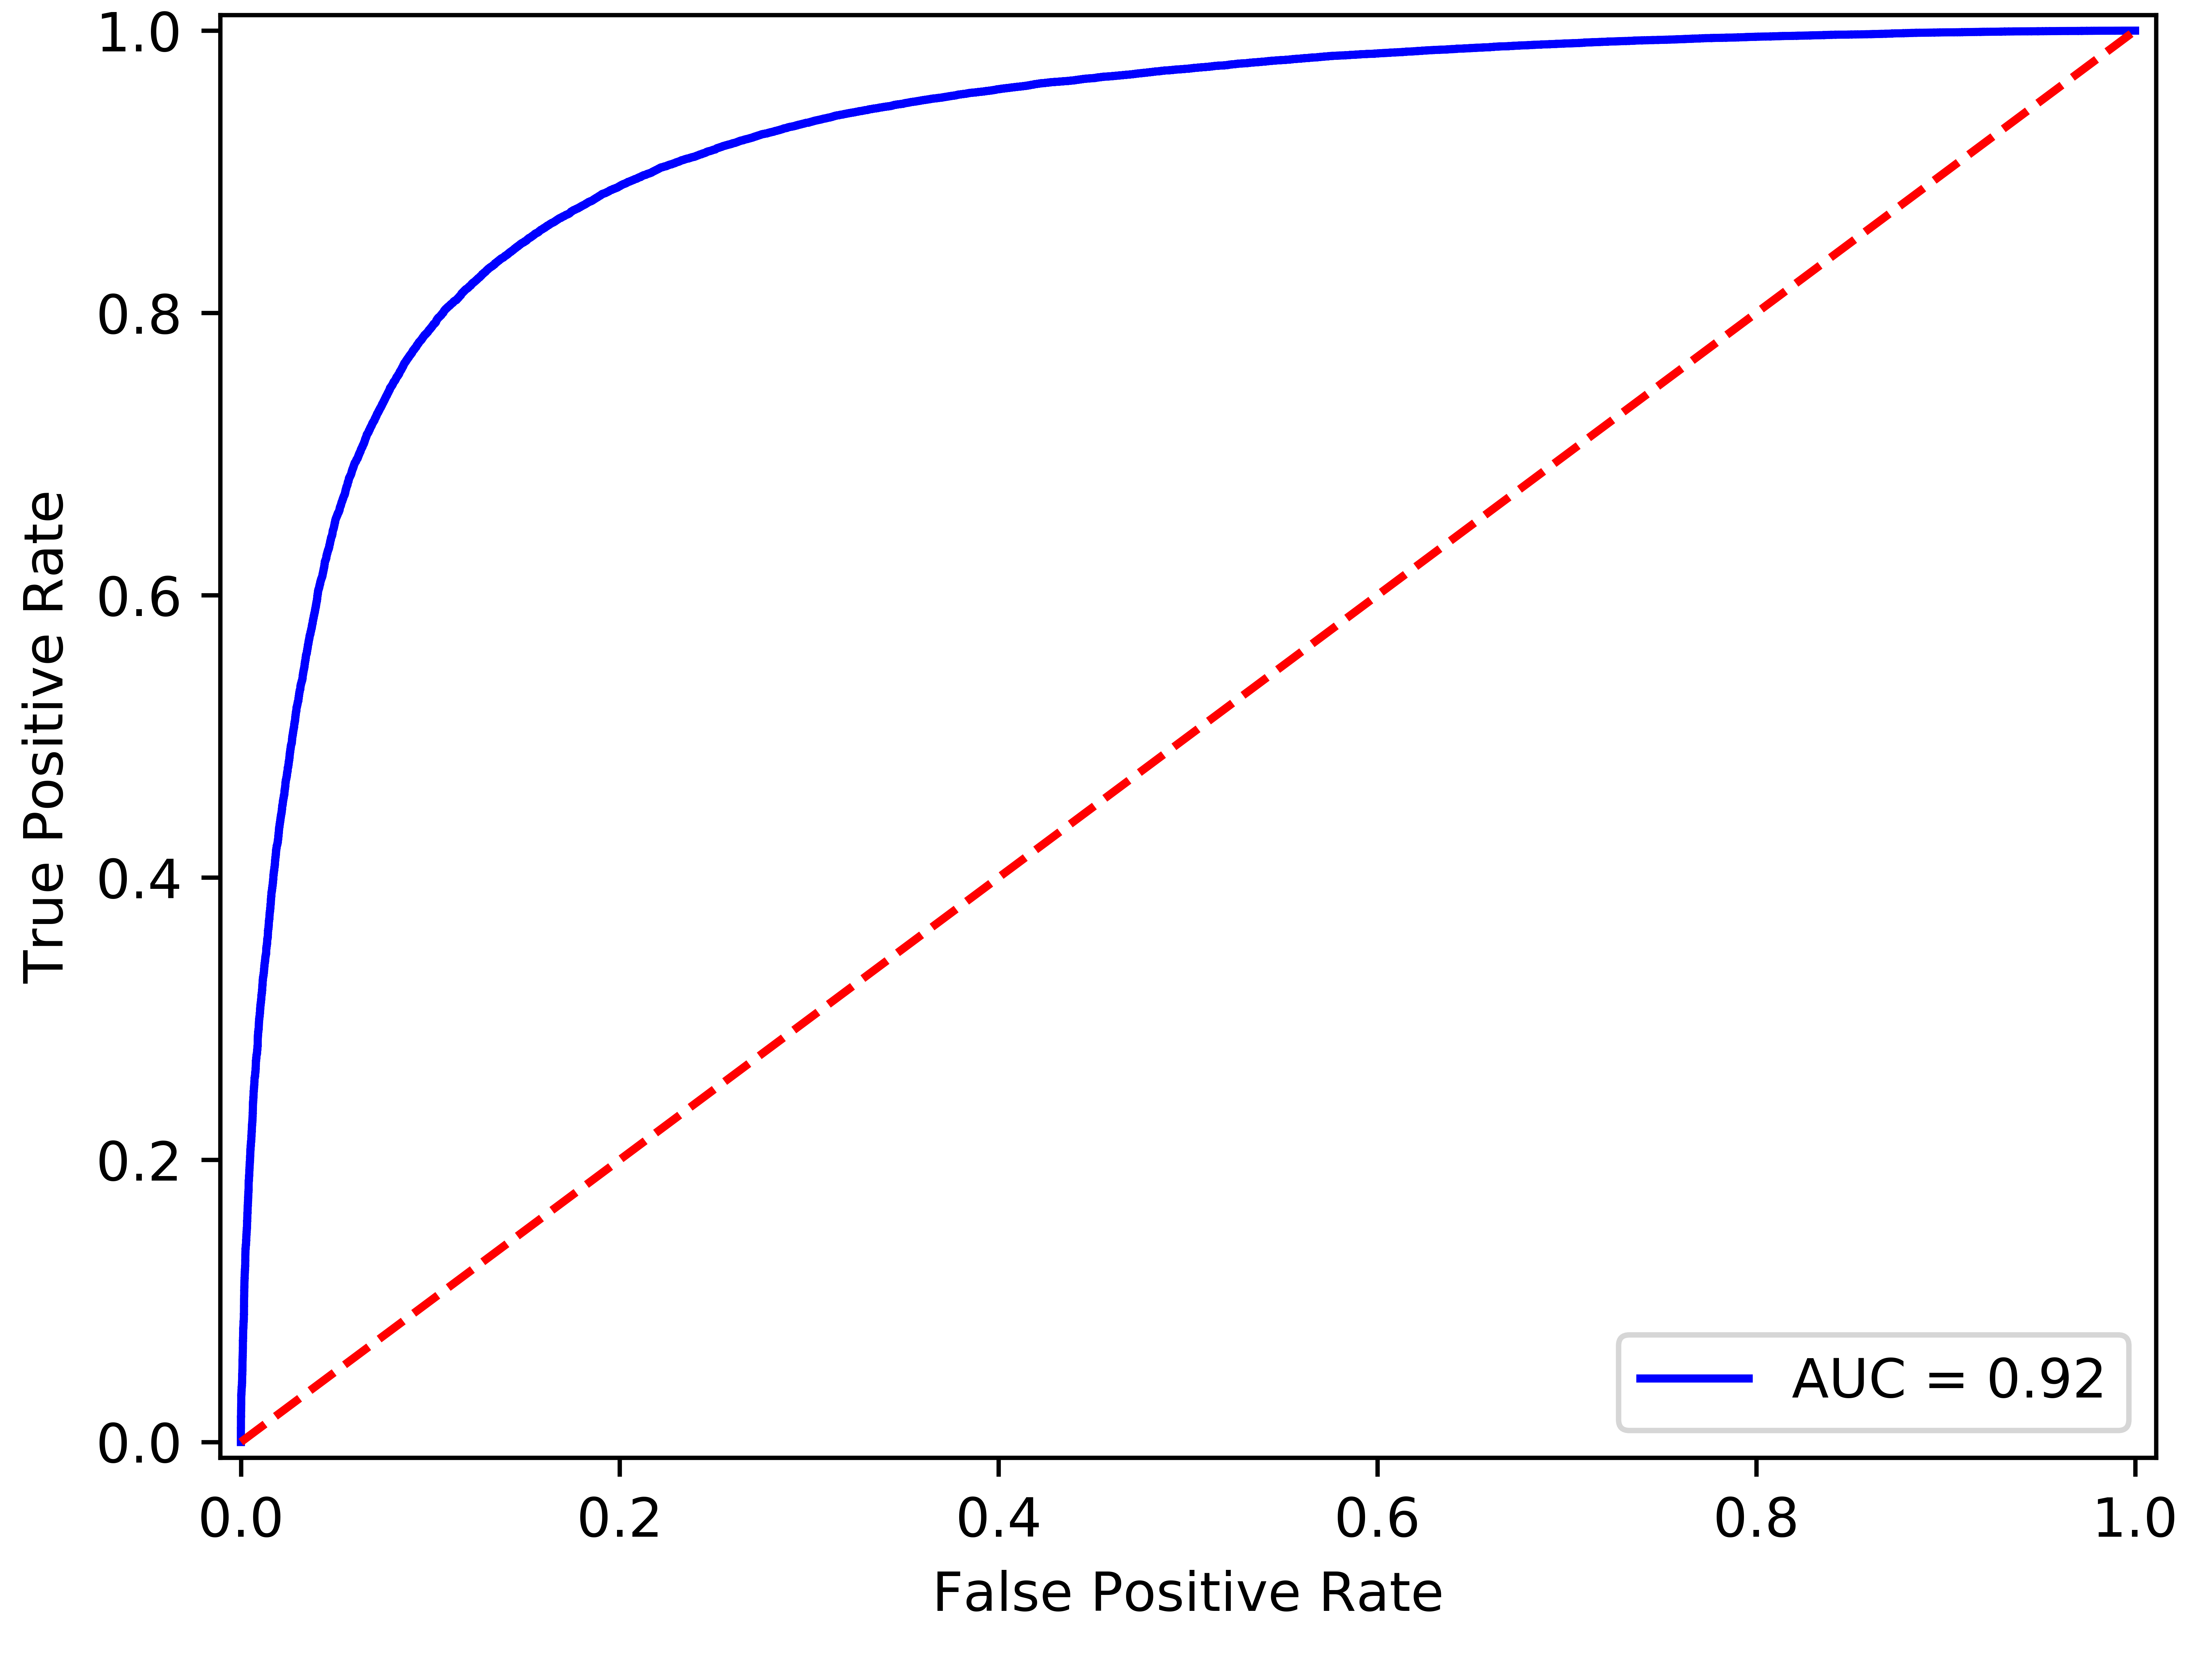
\includegraphics[width=\linewidth,height=.2\textheight,keepaspectratio]{other/insurance_ROC.png}
% \end{subfigure}%
% \hspace{5mm}%
% \begin{subfigure}[t]{.5\linewidth}
%     \centering
%     \captionsetup[subfigure]{}
%     \caption{Summary of most impactful features for financial class.}\label{fig:shapsuminsurance}
%     \includegraphics[width=\linewidth,keepaspectratio]{other/insurance_SHAP_summary.png}
% \end{subfigure}%

% % \noindent
% % \rule[1ex]{width=\linewidth}{0.5pt}
% \caption{\textbf{Prediction of Patient Characteristics.} \\
% Model performance curves are shown for binary classification (Panels \ref{fig:rocgender}, \ref{fig:rocrace}, \ref{fig:rocinsurance}).
% Panels \ref{fig:shapsumgender}, \ref{fig:shapsumrace}, \ref{fig:shapsuminsurance} 
% show the most impactful features on prediction, 
% along with the impact of high or low values for numeric features.
% }\label{fig:otherfig}
% \end{adjustbox}
% \end{figure}
% \clearpage
% \pagestyle{fancy}%
% % \noindent
% % \rule[1ex]{width=\linewidth}{0.5pt}
% % in{minipage}[t][0.5\textheight][t]{\textwidth} %%
\begintables
% \begin{tabular}{L{20em}C{10em}C{10em}C{10em}C{10em}C{10em}}
\toprule
                          \textbf{Characteristic}  &                                       \textbf{}  &  \textbf{Overall}  & \textbf{Not readmitted within 30 days}  & \textbf{Readmitted within 30 days}  & \textbf{Hospital stay less than 7 days}  & \textbf{Hospital stay over 7 days}  \\
\midrule
                                                 n &                                    \hspace{3mm}  &            1485889 &                                 1273593 &                              212296 &                                  1234154 &                              251735 \\
                               Age, median [Q1,Q3] &                                    \hspace{3mm}  &   59.0 [39.0,73.0] &                        59.0 [38.0,73.0] &                    62.0 [48.0,76.0] &                         58.0 [36.0,72.0] &                    66.0 [54.0,78.0] \\
                                     Gender, n (\%) &                              \hspace{3mm} Female &      688352 (55.6) &                           591160 (55.9) &                        97192 (53.4) &                            581139 (56.6) &                       107213 (50.5) \\
                             Race/Ethnicity, n (\%) &                               \hspace{3mm} Black &      275885 (22.3) &                           226842 (21.5) &                        49043 (26.9) &                            228606 (22.3) &                        47279 (22.3) \\
                                                   &                               \hspace{3mm} Other &        76125 (6.1) &                             66482 (6.3) &                          9643 (5.3) &                              66006 (6.4) &                         10119 (4.8) \\
                                                   &                               \hspace{3mm} White &      887057 (71.6) &                           763572 (72.2) &                       123485 (67.8) &                            732202 (71.3) &                       154855 (73.0) \\
                             Marital status, n (\%) &               \hspace{3mm} Divorced or separated &       113045 (9.1) &                             93201 (8.8) &                        19844 (10.9) &                              91295 (8.9) &                        21750 (10.2) \\
                                                   &                \hspace{3mm} Married or partnered &      505950 (40.8) &                           437586 (41.4) &                        68364 (37.5) &                            419966 (40.9) &                        85984 (40.5) \\
                                                   &                               \hspace{3mm} Other &        21211 (1.7) &                             18293 (1.7) &                          2918 (1.6) &                              17274 (1.7) &                          3937 (1.9) \\
                                                   &                              \hspace{3mm} Single &      452229 (36.5) &                           385914 (36.5) &                        66315 (36.4) &                            383525 (37.4) &                        68704 (32.4) \\
                                                   &                             \hspace{3mm} Widowed &      146632 (11.8) &                           121902 (11.5) &                        24730 (13.6) &                            114754 (11.2) &                        31878 (15.0) \\
                            Financial Class, n (\%) &                            \hspace{3mm} Medicaid &      207129 (16.7) &                           175359 (16.6) &                        31770 (17.4) &                            180675 (17.6) &                        26454 (12.5) \\
                                                   &                            \hspace{3mm} Medicare &      658712 (53.2) &                           545109 (51.6) &                       113603 (62.4) &                            515167 (50.2) &                       143545 (67.6) \\
                                                   &                               \hspace{3mm} Other &        72126 (5.8) &                             64829 (6.1) &                          7297 (4.0) &                              64236 (6.3) &                          7890 (3.7) \\
                                                   &            \hspace{3mm} Private health insurance &      301100 (24.3) &                           271599 (25.7) &                        29501 (16.2) &                            266736 (26.0) &                        34364 (16.2) \\
                                     Cancer, n (\%) &                                 \hspace{3mm} 1.0 &      162476 (13.1) &                           126181 (11.9) &                        36295 (19.9) &                            124547 (12.1) &                        37929 (17.9) \\
                     Metastatic solid tumor, n (\%) &                                 \hspace{3mm} 1.0 &        49163 (4.0) &                             36925 (3.5) &                         12238 (6.7) &                              37353 (3.6) &                         11810 (5.6) \\
                     Solid organ transplant, n (\%) &                                 \hspace{3mm} 1.0 &        31102 (2.5) &                             23013 (2.2) &                          8089 (4.4) &                              21069 (2.1) &                         10033 (4.7) \\
                                   AIDS/HIV, n (\%) &                                 \hspace{3mm} 1.0 &         4009 (0.3) &                              2903 (0.3) &                          1106 (0.6) &                               3282 (0.3) &                           727 (0.3) \\
                              Renal disease, n (\%) &                                 \hspace{3mm} 1.0 &      160700 (13.0) &                           120439 (11.4) &                        40261 (22.1) &                            117272 (11.4) &                        43428 (20.5) \\
                         Mild liver disease, n (\%) &                                 \hspace{3mm} 1.0 &        84017 (6.8) &                             63748 (6.0) &                        20269 (11.1) &                              65721 (6.4) &                         18296 (8.6) \\
           Moderate or severe liver disease, n (\%) &                                 \hspace{3mm} 1.0 &        20435 (1.6) &                             13846 (1.3) &                          6589 (3.6) &                              14330 (1.4) &                          6105 (2.9) \\
         Diabetes with chronic complication, n (\%) &                                 \hspace{3mm} 1.0 &       114156 (9.2) &                             87151 (8.2) &                        27005 (14.8) &                              87571 (8.5) &                        26585 (12.5) \\
      Diabetes without chronic complication, n (\%) &                                 \hspace{3mm} 1.0 &      260956 (21.1) &                           206289 (19.5) &                        54667 (30.0) &                            202552 (19.7) &                        58404 (27.5) \\
                               Hypertension, n (\%) &                                   \hspace{3mm} 1 &      804686 (64.9) &                           665818 (63.0) &                       138868 (76.2) &                            639567 (62.3) &                       165119 (77.8) \\
                      Myocardial infarction, n (\%) &                                 \hspace{3mm} 1.0 &        63728 (5.1) &                             48427 (4.6) &                         15301 (8.4) &                              48281 (4.7) &                         15447 (7.3) \\
                                        CHF, n (\%) &                                 \hspace{3mm} 1.0 &      192613 (15.5) &                           147257 (13.9) &                        45356 (24.9) &                            139910 (13.6) &                        52703 (24.8) \\
                    Cerebrovascular disease, n (\%) &                                 \hspace{3mm} 1.0 &      171964 (13.9) &                           137215 (13.0) &                        34749 (19.1) &                            132321 (12.9) &                        39643 (18.7) \\
                                       COPD, n (\%) &                                 \hspace{3mm} 1.0 &      271049 (21.9) &                           214698 (20.3) &                        56351 (30.9) &                            214420 (20.9) &                        56629 (26.7) \\
                                  Pneumonia, n (\%) &                                 \hspace{3mm} 1.0 &      170298 (13.7) &                           127995 (12.1) &                        42303 (23.2) &                            129056 (12.6) &                        41242 (19.4) \\
                                   Dementia, n (\%) &                                 \hspace{3mm} 1.0 &        50458 (4.1) &                             40250 (3.8) &                         10208 (5.6) &                              37056 (3.6) &                         13402 (6.3) \\
                                    Anxiety, n (\%) &                                 \hspace{3mm} 1.0 &      164333 (13.3) &                           131980 (12.5) &                        32353 (17.8) &                            136495 (13.3) &                        27838 (13.1) \\
                                 Depression, n (\%) &                                 \hspace{3mm} 1.0 &      231668 (18.7) &                           184991 (17.5) &                        46677 (25.6) &                            190070 (18.5) &                        41598 (19.6) \\
                                  Psychosis, n (\%) &                                 \hspace{3mm} 1.0 &        46885 (3.8) &                             35074 (3.3) &                         11811 (6.5) &                              34929 (3.4) &                         11956 (5.6) \\
                         Receiving dialysis, n (\%) &                                   \hspace{3mm} 1 &        15808 (1.3) &                             11176 (1.1) &                          4632 (2.5) &                               9495 (0.9) &                          6313 (3.0) \\
 On total parenteral nutrition before or during... &                                 \hspace{3mm} 1.0 &        11052 (0.9) &                              8125 (0.8) &                          2927 (1.6) &                               9437 (0.9) &                          1615 (0.8) \\
    Low hemoglobin level (<12) at discharge, n (\%) &                                   \hspace{3mm} 1 &      205853 (16.6) &                           168088 (15.9) &                        37765 (20.7) &                            165978 (16.2) &                        39875 (18.8) \\
       Low sodium level (<135) at discharge, n (\%) &                                   \hspace{3mm} 1 &        32602 (2.6) &                             26315 (2.5) &                          6287 (3.5) &                              24761 (2.4) &                          7841 (3.7) \\
 Total ED visits in the last 6 months, median [... &                                    \hspace{3mm}  &      0.0 [0.0,1.0] &                           0.0 [0.0,1.0] &                       1.0 [0.0,3.0] &                            0.0 [0.0,1.0] &                       0.0 [0.0,2.0] \\
 Number of patients with any ED visits in past ... &                                   \hspace{3mm} Y &      548326 (44.3) &                           433374 (41.0) &                       114952 (63.1) &                            444750 (43.3) &                       103576 (48.8) \\
                       Admitted from the ED, n (\%) &                                 \hspace{3mm} 1.0 &      605405 (48.9) &                           499960 (47.3) &                       105445 (57.9) &                            516644 (50.3) &                        88761 (41.8) \\
         Previous hospitalizations, median [Q1,Q3] &                                    \hspace{3mm}  &      1.0 [0.0,2.0] &                           0.0 [0.0,2.0] &                       2.0 [0.0,6.0] &                            1.0 [0.0,2.0] &                       1.0 [0.0,3.0] \\
                            Admission class, n (\%) &      \hspace{3mm} Ambulatory Surgical Procedures &         7524 (0.6) &                              6959 (0.7) &                           565 (0.3) &                               7505 (0.7) &                            19 (0.0) \\
                                                   &                           \hspace{3mm} Emergency &         5646 (0.5) &                              5110 (0.5) &                           536 (0.3) &                               5643 (0.5) &                             3 (0.0) \\
                                                   &                             \hspace{3mm} Hospice &         1245 (0.1) &                              1225 (0.1) &                            20 (0.0) &                               1133 (0.1) &                           112 (0.1) \\
                                                   &                           \hspace{3mm} Inpatient &      981357 (79.2) &                           831882 (78.7) &                       149475 (82.1) &                            772265 (75.2) &                       209092 (98.5) \\
                                                   &                         \hspace{3mm} Observation &      232819 (18.8) &                           202314 (19.1) &                        30505 (16.7) &                            231883 (22.6) &                           936 (0.4) \\
                                                   &                               \hspace{3mm} Other &         3671 (0.3) &                              3414 (0.3) &                           257 (0.1) &                               2750 (0.3) &                           921 (0.4) \\
                                                   &                          \hspace{3mm} Outpatient &         3607 (0.3) &                              3222 (0.3) &                           385 (0.2) &                               3581 (0.3) &                            26 (0.0) \\
                                                   &               \hspace{3mm} Psychiatric inpatient &         3198 (0.3) &                              2770 (0.3) &                           428 (0.2) &                               2054 (0.2) &                          1144 (0.5) \\
                         Discharge location, n (\%) &                             \hspace{3mm} Expired &        15345 (1.2) &                             15345 (1.5) &                                     &                               8927 (0.9) &                          6418 (3.0) \\
                                                   &         \hspace{3mm} General Acute Care Hospital &        18313 (1.5) &                             15673 (1.5) &                          2640 (1.4) &                              14893 (1.5) &                          3420 (1.6) \\
                                                   &                                \hspace{3mm} Home &      876280 (70.7) &                           759267 (71.8) &                       117013 (64.2) &                            787787 (76.7) &                        88493 (41.7) \\
                                                   &                  \hspace{3mm} Home Care Services &      128747 (10.4) &                            104368 (9.9) &                        24379 (13.4) &                              89870 (8.8) &                        38877 (18.3) \\
                                                   &                             \hspace{3mm} Hospice &        12761 (1.0) &                             12258 (1.2) &                           503 (0.3) &                               7926 (0.8) &                          4835 (2.3) \\
                                                   &          \hspace{3mm} Intermediate care facility &         8197 (0.7) &                              6726 (0.6) &                          1471 (0.8) &                               4736 (0.5) &                          3461 (1.6) \\
                                                   &         \hspace{3mm} Left Against Medical Advice &        11920 (1.0) &                              8941 (0.8) &                          2979 (1.6) &                              11489 (1.1) &                           431 (0.2) \\
                                                   &             \hspace{3mm} Long-Term Care Facility &        13431 (1.1) &                             11205 (1.1) &                          2226 (1.2) &                               5044 (0.5) &                          8387 (4.0) \\
                                                   &                               \hspace{3mm} Other &         6129 (0.5) &                              5318 (0.5) &                           811 (0.4) &                               4083 (0.4) &                          2046 (1.0) \\
                                                   &            \hspace{3mm} Skilled nursing facility &      137840 (11.1) &                           108813 (10.3) &                        29027 (15.9) &                              83148 (8.1) &                        54692 (25.8) \\
                                                   &  \hspace{3mm} Transfer to a psychiatric hospital &         6047 (0.5) &                              5424 (0.5) &                           623 (0.3) &                               5481 (0.5) &                           566 (0.3) \\
                                                   &        \hspace{3mm} Transfer to another hospital &         4057 (0.3) &                              3558 (0.3) &                           499 (0.3) &                               3430 (0.3) &                           627 (0.3) \\
         Days since last discharge, median [Q1,Q3] &                                    \hspace{3mm}  &  98.1 [24.9,353.4] &                      122.0 [31.4,406.6] &                   41.4 [13.4,152.7] &                       110.7 [27.4,386.0] &                   58.2 [17.1,209.0] \\
                        30-day readmissions, n (\%) &                                   \hspace{3mm} 1 &      182171 (14.7) &                                         &                      182171 (100.0) &                            137221 (13.4) &                        44950 (21.2) \\
            Length of stay in days, median [Q1,Q3] &                                    \hspace{3mm}  &      2.9 [1.7,5.3] &                           2.8 [1.6,5.1] &                       3.9 [2.0,7.0] &                            2.4 [1.4,3.9] &                     10.6 [8.3,15.0] \\
\bottomrule
\end{tabular}

\rowcolors{3}{}{NEJMAlternatingRows}%
\begin{adjustbox}{width={\textwidth},totalheight={\textheight},keepaspectratio,frame,padding=0ex 0ex -910ex 0ex}%
\sffamily %
% \renewcommand\theadalign{cl}
% \renewcommand\theadgape{\Gape[4pt]}
% \renewcommand\theadfont{\normalsize}
{%
\begin{tabular}{L{20em}C{10em}C{10em}C{10em}C{10em}C{10em}}%
\rowcolor{NEJMTopRow} \multicolumn{6}{l}%
{{\textbf{\color{NEJMRed} Table 1.}}%
\textbf{Characteristics  of Hospital Encounters in the Study Sample, Overall and According to Readmission and Extended Length of Stay.}}\\[10pt]%
\hline%
& & & & & \\%
\textbf{Characteristic} & \textbf{Overall} & \textbf{Not readmitted within 30 days} & \textbf{Readmitted within 30 days} & \textbf{Hospital stay less than 7 days} & \textbf{Hospital stay over 7 days}\\
&  &  &  &  & \\
Number of hospitalizations & 1485880 & 1274858 & 211022 & 1234148 & 251732\\
&  &  &  &  & \\
Age, median [Q1,Q3] & 59.0 [39.0,73.0] & 59.0 [38.0,73.0] & 62.0 [48.0,76.0] & 58.0 [36.0,72.0] & 66.0 [54.0,78.0]\\
&  &  &  &  & \\
Gender, n (\%) & &    &     &        &         \\
\hspace{3mm} Female & 826025 (55.6) & 713391 (56.0) & 112634 (53.4) & 698382 (56.6) & 127643 (50.7)\\
&  &  &  &  & \\
Race/Ethnicity, n (\%) & &    &     &        &         \\
\hspace{3mm} African American & 333212 (22.4) & 276208 (21.7) & 57004 (27.0) & 276476 (22.4) & 56736 (22.5)\\
\hspace{3mm} White & 1055180 (71.1) & 913085 (71.7) & 142095 (67.4) & 873453 (70.8) & 181727 (72.2)\\
\hspace{3mm} Other & 96592 (6.5) & 84755 (6.7) & 11837 (5.6) & 83453 (6.8) & 13139 (5.2)\\
&  &  &  &  & \\
Marital status, n (\%)  & &    &     &        &         \\
\hspace{3mm} Divorced or separated & 134841 (9.1) & 111680 (8.8) & 23161 (11.0) & 108779 (8.8) & 26062 (10.4)\\
\hspace{3mm} Married or partnered & 594375 (40.0) & 515620 (40.5) & 78755 (37.3) & 494338 (40.1) & 100037 (39.7)\\
\hspace{3mm} Single & 554116 (37.3) & 477592 (37.5) & 76524 (36.3) & 472301 (38.3) & 81815 (32.5)\\
\hspace{3mm} Widowed & 175822 (11.8) & 146611 (11.5) & 29211 (13.8) & 136888 (11.1) & 38934 (15.5)\\
\hspace{3mm} Other & 26200 (1.8) & 22847 (1.8) & 3353 (1.6) & 21347 (1.7) & 4853 (1.9)\\
&  &  &  &  & \\
Payer Class, n (\%)  & &    &     &        &         \\
\hspace{3mm} Medicaid & 221969 (16.4) & 188630 (16.3) & 33339 (17.0) & 193978 (17.2) & 27991 (12.1)\\
\hspace{3mm} Medicare & 725125 (53.5) & 601752 (51.9) & 123373 (63.0) & 567435 (50.5) & 157690 (68.4)\\
\hspace{3mm} Private health insurance & 329842 (24.3) & 298444 (25.7) & 31398 (16.0) & 293292 (26.1) & 36550 (15.9)\\
\hspace{3mm} Other & 78269 (5.8) & 70553 (6.1) & 7716 (3.9) & 69940 (6.2) & 8329 (3.6)\\
&  &  &  &  & \\
Comorbidities, n (\%)   & &    &     &        &         \\
\hspace{3mm} Cancer &  183367 (12.3) & 142205 (11.2) & 41162 (19.5) & 140188 (11.4) & 43179 (17.2)\\
\hspace{3mm} Metastatic solid tumor & 55906 (3.8) & 41867 (3.3) & 14039 (6.7) & 42339 (3.4) & 13567 (5.4)\\
\hspace{3mm} Solid organ transplant & 33780 (2.3) & 24928 (2.0) & 8852 (4.2) & 22837 (1.9) & 10943 (4.3)\\
\hspace{3mm} AIDS/HIV & 4552 (0.3) & 3310 (0.3) & 1242 (0.6) & 3703 (0.3) & 849 (0.3)\\
\hspace{3mm} Renal disease  & 177544 (11.9) & 133099 (10.4) & 44445 (21.1) & 129114 (10.5) & 48430 (19.2)\\
\hspace{3mm} Mild liver disease & 93947 (6.3) & 71396 (5.6) & 22551 (10.7) & 73362 (5.9) & 20585 (8.2)\\
\hspace{3mm} Moderate or severe liver disease & 22816 (1.5) & 15542 (1.2) & 7274 (3.4) & 15971 (1.3) & 6845 (2.7)\\
\hspace{3mm} Diabetes with chronic complication & 125118 (8.4) & 95619 (7.5) & 29499 (14.0) & 95561 (7.7) & 29557 (11.7)\\
\hspace{3mm} Diabetes without chronic complication & 293379 (19.7) & 232187 (18.2) & 61192 (29.0) & 226901 (18.4) & 66478 (26.4)\\
\hspace{3mm} Hypertension & 939048 (63.2) & 779460 (61.1) & 159588 (75.6) & 744603 (60.3) & 194445 (77.2)\\
\hspace{3mm} Myocardial infarction & 69914 (4.7) & 53267 (4.2) & 16647 (7.9) & 52835 (4.3) & 17079 (6.8)\\
\hspace{3mm} Congestive heart failure & 215510 (14.5) & 164879 (12.9) & 50631 (24.0) & 155898 (12.6) & 59612 (23.7)\\
\hspace{3mm} Cerebrovascular disease & 193243 (13.0) & 154368 (12.1) & 38875 (18.4) & 148158 (12.0) & 45085 (17.9)\\
\hspace{3mm} Chronic obstructive pulmonary disease  & 302548 (20.4) & 240195 (18.8) & 62353 (29.5) & 238907 (19.4) & 63641 (25.3)\\
\hspace{3mm} Pneumonia & 188684 (12.7) & 142066 (11.1) & 46618 (22.1) & 142437 (11.5) & 46247 (18.4)\\
\hspace{3mm} Dementia & 56876 (3.8) & 45461 (3.6) & 11415 (5.4) & 41554 (3.4) & 15322 (6.1)\\
\hspace{3mm} Anxiety & 181440 (12.2) & 146263 (11.5) & 35177 (16.7) & 150668 (12.2) & 30772 (12.2)\\
\hspace{3mm} Depression & 259323 (17.5) & 207914 (16.3) & 51409 (24.4) & 212806 (17.2) & 46517 (18.5)\\
\hspace{3mm} Psychosis & 52085 (3.5) & 39086 (3.1) & 12999 (6.2) & 38544 (3.1) & 13541 (5.4)\\
\hspace{3mm} Receiving dialysis & 17791 (1.2) & 12604 (1.0) & 5187 (2.5) & 10658 (0.9) & 7133 (2.8)\\
&  &  &  &  & \\
Selected discharge laboratory results, n (\%) &  &  &  &  &  \\
\hspace{3mm} Low hemoglobin level (<12 g/dL) & 248387 (16.7) & 204139 (16.0) & 44248 (21.0) & 200374 (16.2) & 48013 (19.1)\\
\hspace{3mm} Low sodium level (<135 mEq/L) & 38847 (2.6) & 31439 (2.5) & 7408 (3.5) & 29467 (2.4) & 9380 (3.7)\\
&  &  &  &  & \\
\makecell[l]{Hospital encounter information, \\ median [Q1,Q3] or n (\%) } &  &  &  &  &  \\
\hspace{3mm} Previous hospitalizations & 1.0 [0.0,2.0] & 0.0 [0.0,2.0] & 2.0 [0.0,6.0] & 1.0 [0.0,2.0] & 1.0 [0.0,3.0]\\
\hspace{3mm} Emergency department (ED) admission & 725843 (48.8) & 603317 (47.3) & 122526 (58.1) & 618055 (50.1) & 107788 (42.8)\\
\hspace{3mm} Any ED visits in past 6 months & 644102 (43.3) & 511323 (40.1) & 132779 (62.9) & 521248 (42.2) & 122854 (48.8)\\
\hspace{3mm} Total ED visits in the last 6 months & 0.0 [0.0,1.0] & 0.0 [0.0,1.0] & 1.0 [0.0,3.0] & 0.0 [0.0,1.0] & 0.0 [0.0,2.0]\\
&  &  &  &  & \\
Admission class, n (\%) & &    &     &        &         \\
\hspace{3mm} Ambulatory Surgical Procedures & 8081 (0.5) & 7464 (0.6) & 617 (0.3) & 8060 (0.7) & 21 (0.0)\\
\hspace{3mm} Emergency & 7058 (0.5) & 6417 (0.5) & 641 (0.3) & 7055 (0.6) & 3 (0.0)\\
\hspace{3mm} Hospice & 1486 (0.1) & 1463 (0.1) & 23 (0.0) & 1357 (0.1) & 129 (0.1)\\
\hspace{3mm} Inpatient & 1185985 (80.0) & 1011772 (79.6) & 174213 (82.7) & 937614 (76.2) & 248371 (98.7)\\
\hspace{3mm} Observation & 261942 (17.7) & 228559 (18.0) & 33383 (15.8) & 260955 (21.2) & 987 (0.4)\\
\hspace{3mm} Outpatient & 10559 (0.7) & 9415 (0.7) & 1144 (0.5) & 10513 (0.9) & 46 (0.0)\\
\hspace{3mm} Psychiatric inpatient & 3381 (0.2) & 2936 (0.2) & 445 (0.2) & 2198 (0.2) & 1183 (0.5)\\
\hspace{3mm} Other & 4074 (0.3) & 3799 (0.3) & 275 (0.1) & 3082 (0.3) & 992 (0.4)\\
&  &  &  &  & \\
Discharge location, n (\%) & &    &     &        &         \\
\hspace{3mm} Expired & 18615 (1.4) & 18615 (1.6) &  0 (0.0) & 10907 (1.0) & 7708 (3.3)\\
\hspace{3mm} General Acute Care Hospital & 19855 (1.5) & 17490 (1.5) & 2365 (1.2) & 16105 (1.4) & 3750 (1.6)\\
\hspace{3mm} Home & 959559 (71.1) & 833797 (72.2) & 125762 (64.8) & 862810 (77.1) & 96749 (42.0)\\
\hspace{3mm} Home Care Services & 134970 (10.0) & 109327 (9.5) & 25643 (13.2) & 93833 (8.4) & 41137 (17.9)\\
\hspace{3mm} Hospice & 14318 (1.1) & 13765 (1.2) & 553 (0.3) & 8879 (0.8) & 5439 (2.4)\\
\hspace{3mm} Intermediate care facility & 9046 (0.7) & 7451 (0.6) & 1595 (0.8) & 5215 (0.5) & 3831 (1.7)\\
\hspace{3mm} Left Against Medical Advice & 13864 (1.0) & 10599 (0.9) & 3265 (1.7) & 13374 (1.2) & 490 (0.2)\\
\hspace{3mm} Long-Term Care Facility & 14592 (1.1) & 12210 (1.1) & 2382 (1.2) & 5403 (0.5) & 9189 (4.0)\\
\hspace{3mm} Skilled nursing facility & 145882 (10.8) & 115106 (10.0) & 30776 (15.8) & 87530 (7.8) & 58352 (25.3)\\
\hspace{3mm} Transfer to a psychiatric hospital & 6828 (0.5) & 6276 (0.5) & 552 (0.3) & 6197 (0.6) & 631 (0.3)\\
\hspace{3mm} Transfer to another hospital & 4482 (0.3) & 4032 (0.3) & 450 (0.2) & 3797 (0.3) & 685 (0.3)\\
\hspace{3mm} Other & 7109 (0.5) & 6240 (0.5) & 869 (0.4) & 4740 (0.4) & 2369 (1.0)\\
&  &  &  &  & \\
Outcomes of interest &  &  &  &  &  \\
\hspace{3mm} 30-day readmissions, n (\%)  & 211022 (14.2) & 0 (0.0) & 211022 (100.0) & 158577 (12.8) & 52445 (20.8)\\
\hspace{3mm} Length of stay in days, median [Q1,Q3] & 2.9 [1.7,5.3] & 2.8 [1.6,5.1] & 3.9 [2.0,7.0] & 2.4 [1.4,3.9] & 10.6 [8.3,15.0]\\
\end{tabular}
\label{table:table1}
}
\end{adjustbox}
%
% \begin{tabular}{lllllll}
\toprule
{} &                                         Unnamed: 0 &            Overall & Not readmitted within 30 days & Readmitted within 30 days & Hospital stay less than 7 days & Hospital stay over 7 days \\
\midrule
0  &                         Number of hospitalizations &            1485859 &                       1220555 &                    265304 &                        1234132 &                    251727 \\
1  &                                                NaN &                NaN &                           NaN &                       NaN &                            NaN &                       NaN \\
2  &                                Age, median [Q1,Q3] &   59.0 [39.0,73.0] &              58.0 [37.0,73.0] &          63.0 [49.0,76.0] &               58.0 [36.0,72.0] &          66.0 [54.0,78.0] \\
3  &                                                NaN &                NaN &                           NaN &                       NaN &                            NaN &                       NaN \\
4  &                                      Gender, n (\%) &                NaN &                           NaN &                       NaN &                            NaN &                       NaN \\
5  &                                             Female &      688337 (55.6) &                 568101 (56.0) &             120236 (53.5) &                  581129 (56.6) &             107208 (50.5) \\
6  &                                                NaN &                NaN &                           NaN &                       NaN &                            NaN &                       NaN \\
7  &                              Race/Ethnicity, n (\%) &                NaN &                           NaN &                       NaN &                            NaN &                       NaN \\
8  &                                              Black &      275880 (22.3) &                 216925 (21.4) &              58955 (26.2) &                  228601 (22.3) &              47279 (22.3) \\
9  &                                              White &      887036 (71.6) &                 732919 (72.3) &             154117 (68.6) &                  732187 (71.3) &             154849 (73.0) \\
10 &                                              Other &        76124 (6.1) &                   64487 (6.4) &               11637 (5.2) &                    66006 (6.4) &               10118 (4.8) \\
11 &                                                NaN &                NaN &                           NaN &                       NaN &                            NaN &                       NaN \\
12 &                              Marital status, n (\%) &                NaN &                           NaN &                       NaN &                            NaN &                       NaN \\
13 &                               Married or partnered &      505937 (40.8) &                 422396 (41.6) &              83541 (37.2) &                  419956 (40.9) &              85981 (40.5) \\
14 &                              Divorced or separated &       113043 (9.1) &                   88753 (8.7) &              24290 (10.8) &                    91293 (8.9) &              21750 (10.2) \\
15 &                                            Widowed &      146626 (11.8) &                 114874 (11.3) &              31752 (14.1) &                  114750 (11.2) &              31876 (15.0) \\
16 &                                             Single &      452223 (36.5) &                 371022 (36.6) &              81201 (36.1) &                  383521 (37.4) &              68702 (32.4) \\
17 &                                              Other &        21211 (1.7) &                   17286 (1.7) &                3925 (1.7) &                    17274 (1.7) &                3937 (1.9) \\
18 &                                                NaN &                NaN &                           NaN &                       NaN &                            NaN &                       NaN \\
19 &                             Financial class, n (\%) &                NaN &                           NaN &                       NaN &                            NaN &                       NaN \\
20 &                                           Medicaid &      207128 (16.7) &                 169507 (16.7) &              37621 (16.7) &                  180674 (17.6) &              26454 (12.5) \\
21 &                                           Medicare &      658693 (53.2) &                 515824 (50.9) &             142869 (63.6) &                  515154 (50.2) &             143539 (67.6) \\
22 &                           Private Health Insurance &      301095 (24.3) &                 265603 (26.2) &              35492 (15.8) &                  266732 (26.0) &              34363 (16.2) \\
23 &                                              Other &        72124 (5.8) &                   63397 (6.3) &                8727 (3.9) &                    64234 (6.3) &                7890 (3.7) \\
24 &                                                NaN &                NaN &                           NaN &                       NaN &                            NaN &                       NaN \\
25 &                               Comorbidities, n (\%) &                NaN &                           NaN &                       NaN &                            NaN &                       NaN \\
26 &                                             Cancer &      162469 (13.1) &                 119331 (11.8) &              43138 (19.2) &                  124540 (12.1) &              37929 (17.9) \\
27 &                             Metastatic solid tumor &        49159 (4.0) &                   34552 (3.4) &               14607 (6.5) &                    37349 (3.6) &               11810 (5.6) \\
28 &                             Solid organ transplant &        31101 (2.5) &                   21770 (2.1) &                9331 (4.2) &                    21069 (2.1) &               10032 (4.7) \\
29 &                                           AIDS/HIV &         4009 (0.3) &                    2758 (0.3) &                1251 (0.6) &                     3282 (0.3) &                 727 (0.3) \\
30 &                                      Renal disease &      160692 (13.0) &                 112953 (11.1) &              47739 (21.2) &                  117267 (11.4) &              43425 (20.5) \\
31 &                                 Mild liver disease &        84014 (6.8) &                   60243 (5.9) &              23771 (10.6) &                    65720 (6.4) &               18294 (8.6) \\
32 &                   Moderate or severe liver disease &        20434 (1.6) &                   12886 (1.3) &                7548 (3.4) &                    14330 (1.4) &                6104 (2.9) \\
33 &                 Diabetes with chronic complication &       114155 (9.2) &                   81850 (8.1) &              32305 (14.4) &                    87570 (8.5) &              26585 (12.5) \\
34 &              Diabetes without chronic complication &      260951 (21.1) &                 194623 (19.2) &              66328 (29.5) &                  202547 (19.7) &              58404 (27.5) \\
35 &                                       Hypertension &      804663 (64.9) &                 632256 (62.3) &             172407 (76.7) &                  639550 (62.3) &             165113 (77.8) \\
36 &                              Myocardial infarction &        63725 (5.1) &                   45493 (4.5) &               18232 (8.1) &                    48279 (4.7) &               15446 (7.3) \\
37 &                                                CHF &      192606 (15.5) &                 138096 (13.6) &              54510 (24.3) &                  139907 (13.6) &              52699 (24.8) \\
38 &                            Cerebrovascular disease &      171956 (13.9) &                 128106 (12.6) &              43850 (19.5) &                  132314 (12.9) &              39642 (18.7) \\
39 &                                               COPD &      271041 (21.9) &                 203152 (20.0) &              67889 (30.2) &                  214415 (20.9) &              56626 (26.7) \\
40 &                                          Pneumonia &      170288 (13.7) &                 119998 (11.8) &              50290 (22.4) &                  129048 (12.6) &              41240 (19.4) \\
41 &                                           Dementia &        50455 (4.1) &                   37356 (3.7) &               13099 (5.8) &                    37054 (3.6) &               13401 (6.3) \\
42 &                                            Anxiety &      164331 (13.3) &                 125062 (12.3) &              39269 (17.5) &                  136493 (13.3) &              27838 (13.1) \\
43 &                                         Depression &      231666 (18.7) &                 174542 (17.2) &              57124 (25.4) &                  190068 (18.5) &              41598 (19.6) \\
44 &                                          Psychosis &        46884 (3.8) &                   32260 (3.2) &               14624 (6.5) &                    34929 (3.4) &               11955 (5.6) \\
45 &                                                NaN &                NaN &                           NaN &                       NaN &                            NaN &                       NaN \\
46 &                 Selected laboratory results, n (\%) &                NaN &                           NaN &                       NaN &                            NaN &                       NaN \\
47 &            Low hemoglobin level (<12) at discharge &      205848 (16.6) &                 160435 (15.8) &              45413 (20.2) &                  165976 (16.2) &              39872 (18.8) \\
48 &               Low sodium level (<135) at discharge &        32601 (2.6) &                   24672 (2.4) &                7929 (3.5) &                    24760 (2.4) &                7841 (3.7) \\
49 &                                                NaN &                NaN &                           NaN &                       NaN &                            NaN &                       NaN \\
50 &                             Admission class, n (\%) &                NaN &                           NaN &                       NaN &                            NaN &                       NaN \\
51 &                                          Inpatient &      981331 (79.2) &                 793726 (78.3) &             187605 (83.5) &                  772246 (75.2) &             209085 (98.5) \\
52 &                                        Observation &      232818 (18.8) &                 198316 (19.6) &              34502 (15.4) &                  231882 (22.6) &                 936 (0.4) \\
53 &                     Ambulatory Surgical Procedures &         7524 (0.6) &                    6925 (0.7) &                 599 (0.3) &                     7505 (0.7) &                  19 (0.0) \\
54 &                                          Emergency &         5646 (0.5) &                    5045 (0.5) &                 601 (0.3) &                     5643 (0.5) &                   3 (0.0) \\
55 &                              Psychiatric inpatient &         3198 (0.3) &                    2683 (0.3) &                 515 (0.2) &                     2054 (0.2) &                1144 (0.5) \\
56 &                                            Hospice &         1245 (0.1) &                    1207 (0.1) &                  38 (0.0) &                     1133 (0.1) &                 112 (0.1) \\
57 &                                              Other &         3671 (0.3) &                    3258 (0.3) &                 413 (0.2) &                     2750 (0.3) &                 921 (0.4) \\
58 &                                                NaN &                NaN &                           NaN &                       NaN &                            NaN &                       NaN \\
59 &                          Discharge location, n (\%) &                NaN &                           NaN &                       NaN &                            NaN &                       NaN \\
60 &                                               Home &      876280 (70.7) &                 755125 (74.4) &             121155 (53.9) &                  787787 (76.7) &              88493 (41.7) \\
61 &                                 Home care services &      128747 (10.4) &                  100117 (9.9) &              28630 (12.7) &                    89870 (8.8) &              38877 (18.3) \\
62 &                         Intermediate care facility &         8197 (0.7) &                    6545 (0.6) &                1652 (0.7) &                     4736 (0.5) &                3461 (1.6) \\
63 &                           Skilled nursing facility &      137840 (11.1) &                   98848 (9.7) &              38992 (17.4) &                    83148 (8.1) &              54692 (25.8) \\
64 &                            Long-term care facility &        13431 (1.1) &                    8699 (0.9) &                4732 (2.1) &                     5044 (0.5) &                8387 (4.0) \\
65 &                        General acute care hospital &        18313 (1.5) &                    6312 (0.6) &               12001 (5.3) &                    14893 (1.5) &                3420 (1.6) \\
66 &                       Transfer to another hospital &         4057 (0.3) &                     904 (0.1) &                3153 (1.4) &                     3430 (0.3) &                 627 (0.3) \\
67 &                 Transfer to a psychiatric hospital &         6047 (0.5) &                    1081 (0.1) &                4966 (2.2) &                     5481 (0.5) &                 566 (0.3) \\
68 &                        Left against medical advice &        11920 (1.0) &                    8856 (0.9) &                3064 (1.4) &                    11489 (1.1) &                 431 (0.2) \\
69 &                                            Hospice &        12761 (1.0) &                    8809 (0.9) &                3952 (1.8) &                     7926 (0.8) &                4835 (2.3) \\
70 &                                            Expired &        15318 (1.2) &                   15318 (1.5) &                   0 (0.0) &                     8907 (0.9) &                6411 (3.0) \\
71 &                                              Other &         6129 (0.5) &                    3717 (0.4) &                2412 (1.1) &                     4083 (0.4) &                2046 (1.0) \\
72 &                                                NaN &                NaN &                           NaN &                       NaN &                            NaN &                       NaN \\
73 &       Hospital encounter , median [Q1,Q3] or n (\%) &                NaN &                           NaN &                       NaN &                            NaN &                       NaN \\
74 &                          Previous hospitalizations &      1.0 [0.0,2.0] &                 0.0 [0.0,2.0] &             2.0 [0.0,5.0] &                  1.0 [0.0,2.0] &             1.0 [0.0,3.0] \\
75 &                          Days since last discharge &  80.3 [16.6,318.2] &            102.9 [21.3,376.6] &          37.0 [9.9,150.6] &              97.3 [21.1,362.5] &          35.1 [5.6,154.9] \\
76 &               Total ED visits in the last 6 months &      0.0 [0.0,1.0] &                 0.0 [0.0,1.0] &             1.0 [0.0,3.0] &                  0.0 [0.0,1.0] &             0.0 [0.0,2.0] \\
77 &  Number of patients with any ED visits in past ... &      548312 (44.3) &                 410343 (40.5) &             137969 (61.4) &                  444739 (43.3) &             103573 (48.8) \\
78 &                               Admitted from the ED &      605390 (48.9) &                 475509 (46.9) &             129881 (57.8) &                  516634 (50.3) &              88756 (41.8) \\
79 &                                                NaN &                NaN &                           NaN &                       NaN &                            NaN &                       NaN \\
80 &                               Outcomes of interest &                NaN &                           NaN &                       NaN &                            NaN &                       NaN \\
81 &             Length of stay in days, median [Q1,Q3] &      2.9 [1.7,5.3] &                 2.8 [1.6,5.0] &             3.9 [2.0,7.0] &                  2.4 [1.4,3.9] &           10.6 [8.3,15.0] \\
82 &                         30-day readmissions, n (\%) &      265304 (17.9) &                       0 (0.0) &            265304 (100.0) &                  168920 (16.5) &              55789 (26.3) \\
\bottomrule
\end{tabular}
%

% \begin{table}[!htbp]
% \sffamily
% \setlength\tabcolsep{6pt} % default is 6pt
% \rowcolors{3}{}{NEJMAlternatingRows}
% \begin{tabularx}{\textwidth}{lcYYYY}%
% \toprule
% \rowcolor{NEJMTopRow}{{{\textbf{\color{NEJMRed} Table 2.\}}\textbf{Performance of Predictive Models}}} & & & & \\ 
% \midrule
% \textbf{Target} & \textbf{ROC AUC} & \textbf{Brier Score Loss} &   \textbf{RMSE} \\
%                         %   &         &                  &                   &        \\
% Readmitted within 30 days &    0.76 &              0.10 &        -- \\
% Readmitted within 7 days  &     0.70 &             0.04 &        -- \\
% Readmitted within 5 days  &    0.69 &             0.03 &        -- \\
% Readmitted within 3 days  &    0.65 &             0.02 &        -- \\
% Days to readmission       &      -- &               -- &      8.98 \\
% Hospital stay over 7 days &    0.85 &             0.12 &        -- \\
% Hospital stay over 5 days &    0.85 &             0.14 &        -- \\
% Hospital stay over 3 days &    0.86 &             0.15 &        -- \\
% Length of stay (days)            &      -- &               -- &       3.94 \\
% Gender                    &    0.87 &             0.14 &         -- \\
% Race                      &    0.91 &              0.10 &        -- \\
% Financial Class           &    0.92 &              0.10 &        -- \\
% Age over 65 years            & 0.xx    & 0.xx              &       -- \\
% Age (years)                       &      -- &               -- &     10.37 \\
% \bottomrule
% \end{tabularx}
% \label{table:table2}
% \end{table}

\rowcolors{3}{}{NEJMAlternatingRows} 
\begin{adjustbox}{width={\textwidth},keepaspectratio,frame}%
{
\begin{tabular}{lcccc}
\rowcolor{NEJMTopRow} \multicolumn{4}{l}%{\addstackgap[4pt]
{{\textbf{\color{NEJMRed} Table 2.}}
\textbf{Performance of Predictive Models}} 
\\ %\vspace{2.5mm} %[7pt]
\hline
\textbf{Target} & \textbf{ROC AUC} & \textbf{Brier Score Loss} &   \textbf{RMSE} \\
                        %   &         &                  &                   &        \\
Readmitted within 30 days &    0.76 &              0.11 &        -- \\
Readmitted within 7 days  &    0.70 &              0.05 &        -- \\
Readmitted within 5 days  &    0.69 &              0.03 &        -- \\
Readmitted within 3 days  &    0.67 &              0.02 &        -- \\
Days to readmission       &      -- &                -- &      8.98 \\
Death within 48--72 hours &    0.91 &              0.001 &        -- \\
Hospital stay over 7 days &    0.84 &              0.12 &        -- \\
Hospital stay over 5 days &    0.84 &              0.15 &        -- \\
Hospital stay over 3 days &    0.84 &              0.16 &        -- \\
Length of stay (days)     &      -- &                -- &      3.94 \\
Gender                    &    0.88 &              0.14 &        -- \\
Race                      &    0.92 &              0.09 &        -- \\
Payer Class               &    0.92 &              0.10 &        -- \\
Age over 65 years         &    0.94 &              0.09 &        -- \\
Age (years)               &      -- &                -- &     10.37 \\
\end{tabular}
\label{table:table2}
}
\end{adjustbox}



% \rowcolors{3}{}{NEJMAlternatingRows} 
% \begin{adjustbox}{width={\textwidth},keepaspectratio,frame}%
% {
% \begin{tabular}{lcccc}
% \rowcolor{NEJMTopRow} \multicolumn{4}{l}%{\addstackgap[4pt]
% {{\textbf{\color{NEJMRed} Table 2.}}
% \textbf{Performance of Predictive Models}} 
% \\ %\vspace{2.5mm} %[7pt]
% \hline
%     &                 &                            &                        &                   \\
%     \textbf{Target} & \textbf{ROC AUC} & \textbf{Brier Score Loss} & \textbf{Average Precision}&   \textbf{RMSE} \\
%                             %   &         &                  &                   &        \\
%     Readmitted within 30 days &    0.77 &              0.10 &              0.37 &     -- \\
%     Readmitted within 7 days  &     0.70 &             0.04 &              0.11 &     -- \\
%     Readmitted within 5 days  &    0.69 &             0.03 &              0.07 &     -- \\
%     Readmitted within 3 days  &    0.65 &             0.02 &              0.03 &     -- \\
%     Days to readmission       &      -- &               -- &                -- &   8.98 \\
%     Hospital stay over 7 days &    0.85 &             0.12 &              0.58 &     -- \\
%     Hospital stay over 5 days &    0.85 &             0.14 &              0.73 &     -- \\
%     Hospital stay over 3 days &    0.86 &             0.15 &              0.88 &     -- \\
%     Length of stay (days)            &      -- &               -- &                -- &   3.94 \\
%     Gender                    &    0.87 &             0.14 &              0.85 &     -- \\
%     Race                      &    0.91 &              0.10 &              0.86 &     -- \\
%     Financial Class           &    0.92 &              0.10 &              0.96 &     -- \\
%     Age (years)                       &      -- &               -- &                -- &  10.37 \\
% \end{tabular}
% \label{table:table2}
% }
% \end{adjustbox}%%
\beginsupplement\
%
% Figs
\begin{figure}
\begin{adjustbox}{minipage=7.0in,frame}
\vspace{2.5mm}
\centering
%
\def\mpicdir{supplementary/metrics/}
%
\def\mcapbig{Prediction of Patient Characteristics: Metrics.}
\def\mlabbig{fig:supmetrics}
%
% 1
\def\mpicone{gender_cal.pdf}
\def\mcapone{Gender calibration curve.}
\def\mlabone{fig:calgender}
% 2
\def\mpictwo{gender_ROC.pdf}
\def\mcaptwo{Gender AUC curve.}
\def\mlabtwo{fig:aucgender}
% 3
\def\mpicthr{age_cal.pdf}
\def\mcapthr{Age calibration curve.}
\def\mlabthr{fig:calage}
% 4
\def\mpicfor{age_ROC.pdf}
\def\mcapfor{Age ROC curve.}
\def\mlabfor{fig:aucage}
% 5
\def\mpicfiv{insurance_cal.pdf}
\def\mcapfiv{Insurance calibration curve.}
\def\mlabfiv{fig:calinsurance}
% 6
\def\mpicsix{insurance_ROC.pdf}
\def\mcapsix{Insurance ROC curve.}
\def\mlabsix{fig:aucinsurance}
% 7
\def\mpicsev{race_cal.pdf}
\def\mcapsev{Race calibration curve.}
\def\mlabsev{fig:calrace}
% 8
\def\mpicate{race_ROC.pdf}
\def\mcapate{Race ROC curve.}
\def\mlabate{fig:aucrace}
%
%
% \hspace{5mm}%
\begin{subfigure}[t]{.45\linewidth}
    \centering
    \caption{\mcapone}\label{\mlabone}
    \includegraphics[height=2in,width=2in]{\mpicdir\mpicone}
\end{subfigure}%
\begin{subfigure}[t]{.45\linewidth}
    \centering
    \captionsetup[subfigure]{}
    \caption{\mcaptwo}\label{\mlabtwo}
    \vspace{-3mm}
    \includegraphics[height=2in,width=2in]{\mpicdir\mpictwo}
\end{subfigure}%
\vspace{0mm}
\begin{subfigure}[t]{.45\linewidth}
    \centering
    \captionsetup[subfigure]{}
    \caption{\mcapthr}\label{\mlabthr}
    \includegraphics[height=2in,width=2in]{\mpicdir\mpicthr}
\end{subfigure}%
\begin{subfigure}[t]{.45\linewidth}
    \centering
    \captionsetup[subfigure]{}
    \caption{\mcapfor}\label{\mlabfor}
    \vspace{-3mm}
    \includegraphics[height=2in,width=2in]{\mpicdir\mpicfor}
\end{subfigure}%
\vspace{0mm}
\begin{subfigure}[t]{.45\linewidth}
    \centering
    \captionsetup[subfigure]{}
    \caption{\mcapfiv}\label{\mlabfiv}
    \includegraphics[height=2in,width=2in]{\mpicdir\mpicfiv}
\end{subfigure}%
\begin{subfigure}[t]{.45\linewidth}
    \centering
    \captionsetup[subfigure]{}
    \caption{\mcapsix}\label{\mlabsix}
    \vspace{-3mm}
    \includegraphics[height=2in,width=2in]{\mpicdir\mpicsix}
\end{subfigure}%
\vspace{0mm}
\begin{subfigure}[t]{.45\linewidth}
    \centering
    \captionsetup[subfigure]{}
    \caption{\mcapsev.}\label{\mlabsev}
    \includegraphics[height=2in,width=2in]{\mpicdir\mpicsev}
\end{subfigure}%
\begin{subfigure}[t]{.45\linewidth}
    \centering
    \captionsetup[subfigure]{}
    \caption{\mcapate}\label{\mlabate}
    \vspace{-3mm}
    \includegraphics[height=2in,width=2in]{\mpicdir\mpicate}
\end{subfigure}%

\caption{\textbf{\mcapbig} \\
% Panels%
% ~\ref{fig:calgender},~\ref{fig:aucgender},%
% ~\ref{fig:calage},~\ref{fig:aucage},%
% ~\ref{fig:calinsurance},~\ref{fig:aucinsurance},%
% ~\ref{fig:calrace},~\ref{fig:aucrace}
% show performance metrics as indicated.
}\label{\mlabbig}
\end{adjustbox}
\end{figure}
\begin{figure}
\begin{adjustbox}{minipage=1.0\linewidth,frame}
\vspace{2.5mm}
\centering

\begin{subfigure}[t]{.45\linewidth}
    \centering
    \captionsetup[subfigure]{}
    \caption{3-day readmission.}\label{fig:shaprdt3d}
    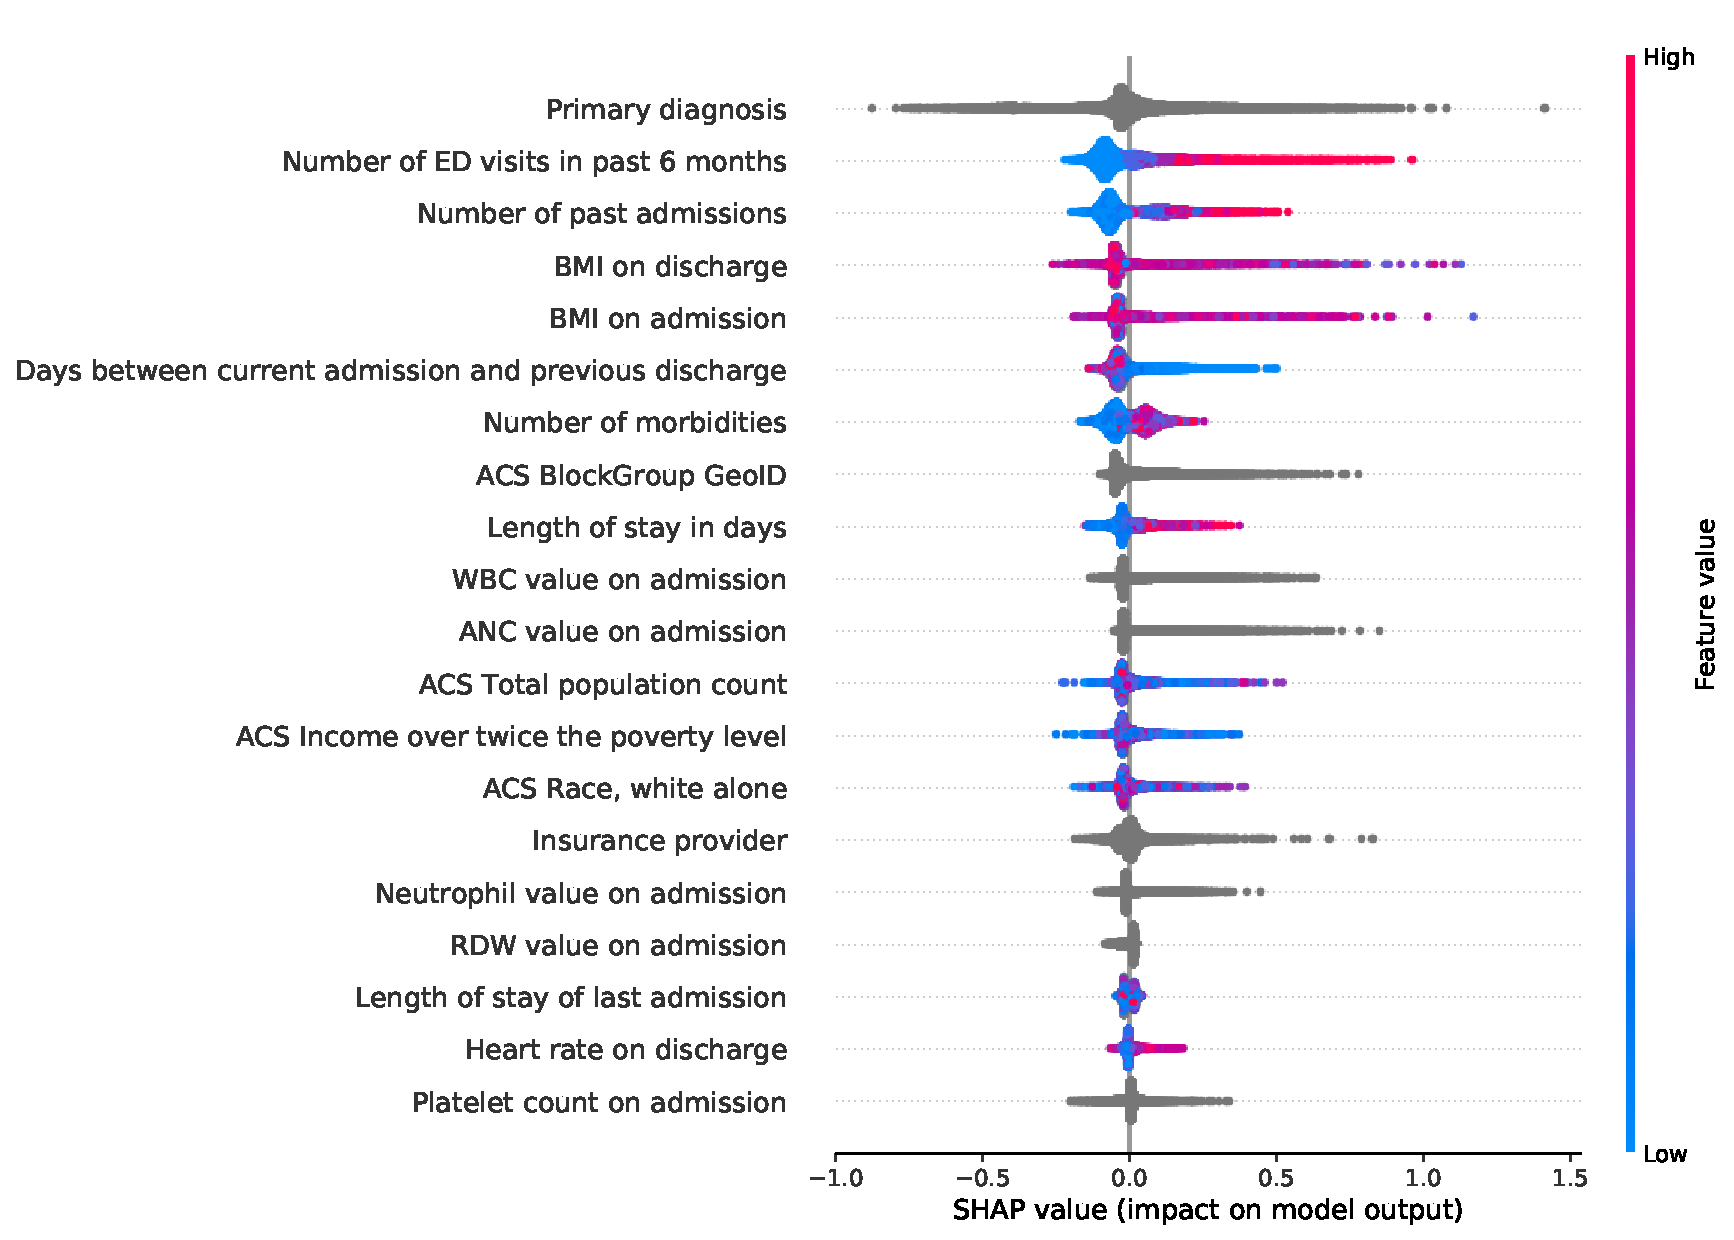
\includegraphics[width=\linewidth,keepaspectratio]{supplementary/readmitted3d_SHAP_summary.pdf}
\end{subfigure}%
\begin{subfigure}[t]{.45\linewidth}
    \centering
    \captionsetup[subfigure]{}
    \caption{7-day readmission.}\label{fig:shaprdt7d}
    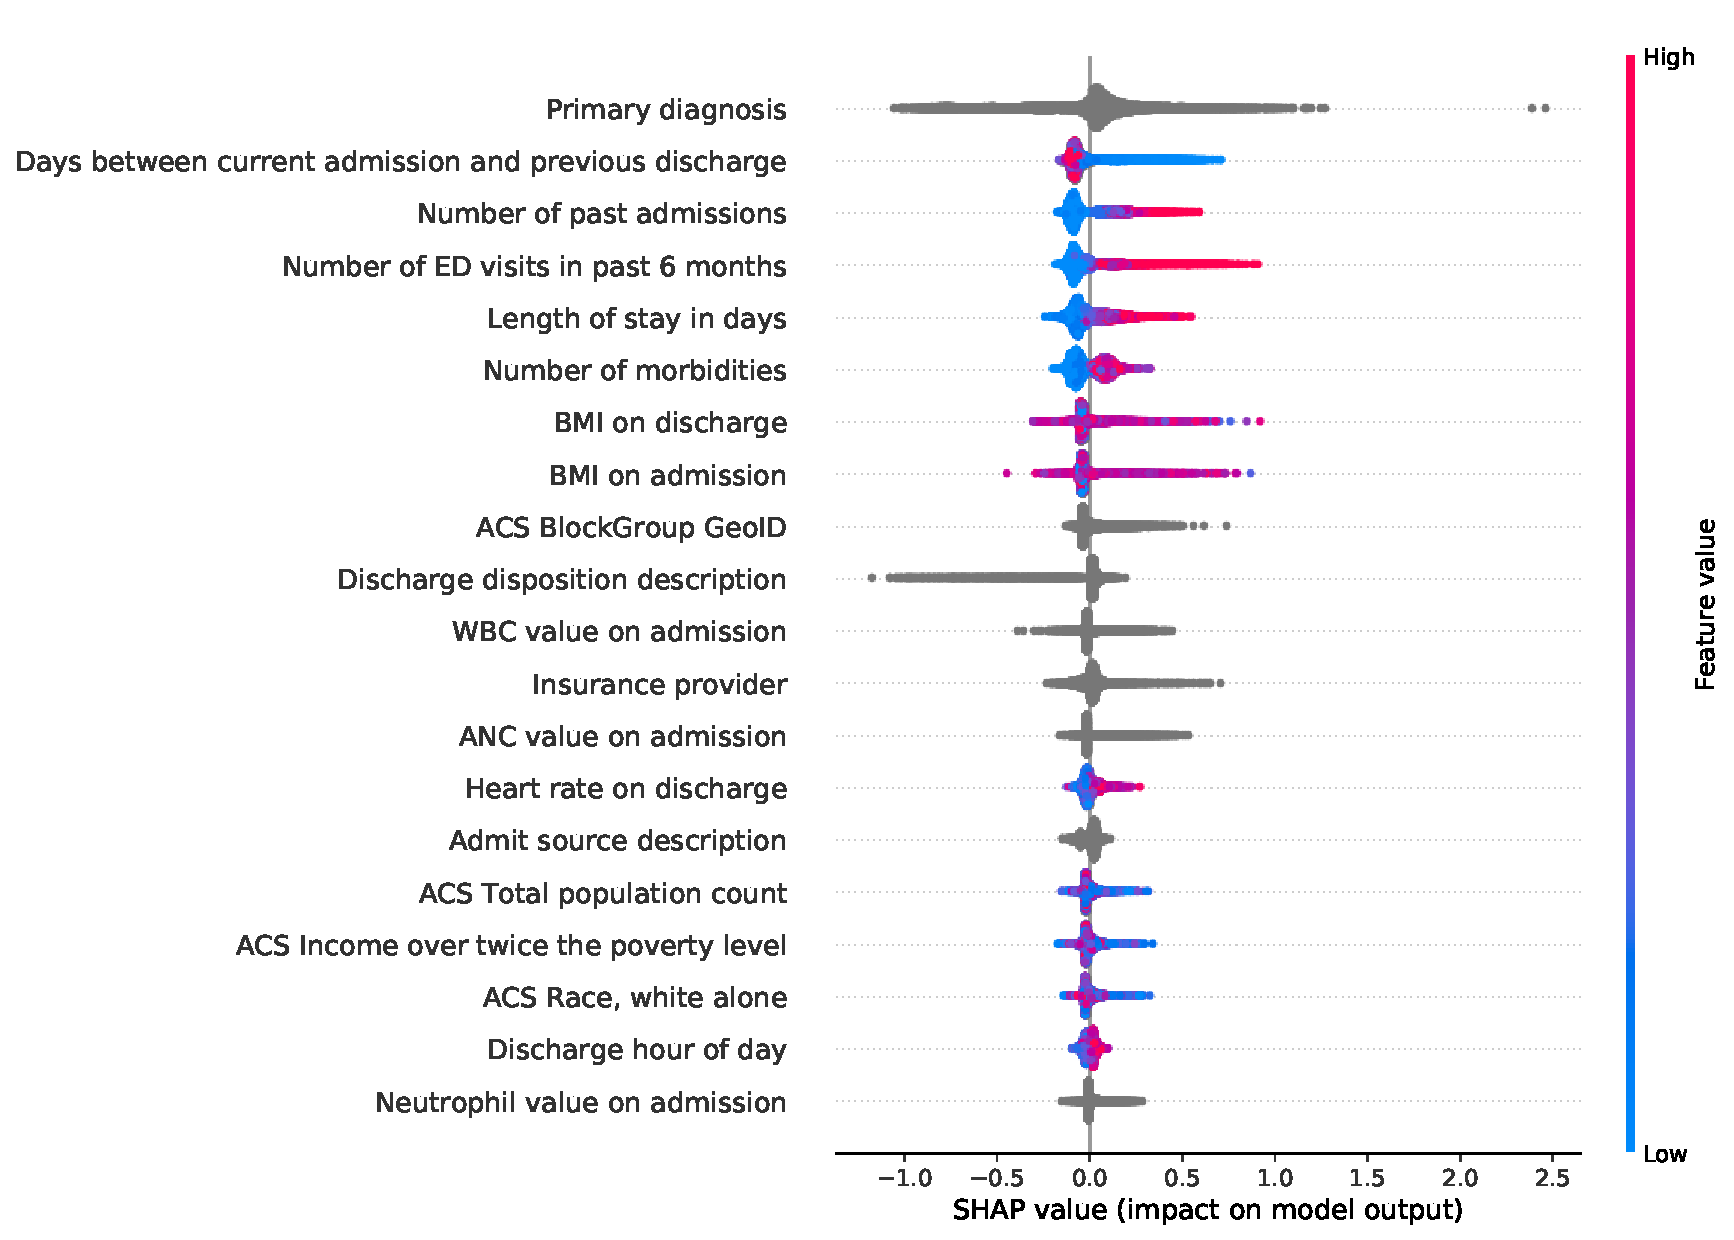
\includegraphics[width=\linewidth,keepaspectratio]{supplementary/readmitted7d_SHAP_summary.pdf}
\end{subfigure}%

\begin{subfigure}[t]{.45\linewidth}
    \centering
    \captionsetup[subfigure]{}
    \caption{Length of stay over 3 days.}\label{fig:shaplos3d}
    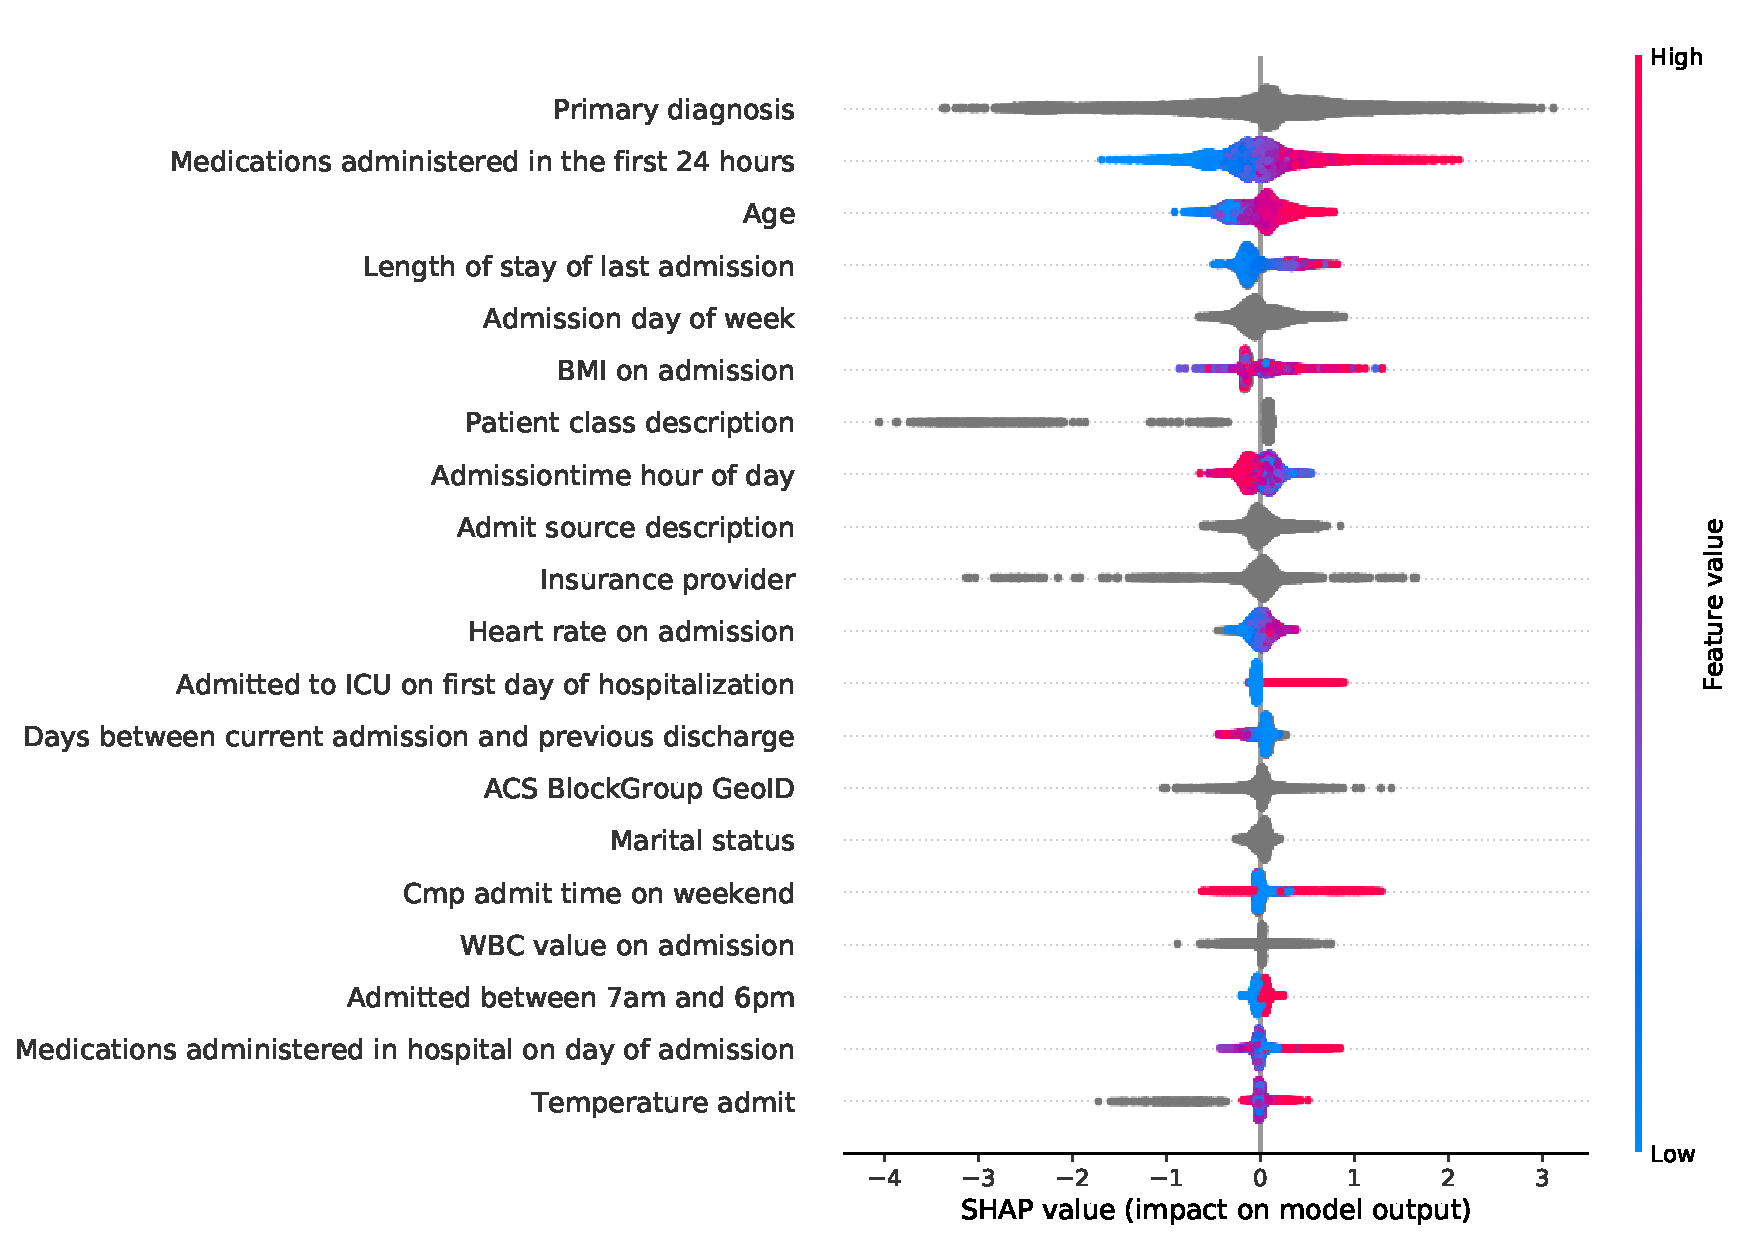
\includegraphics[width=\linewidth,keepaspectratio]{supplementary/los3d_SHAP_summary.pdf}
\end{subfigure}%
\begin{subfigure}[t]{.45\linewidth}
    \centering
    \captionsetup[subfigure]{}
    \caption{Length of stay over 3 days.}\label{fig:shaplos7d}
    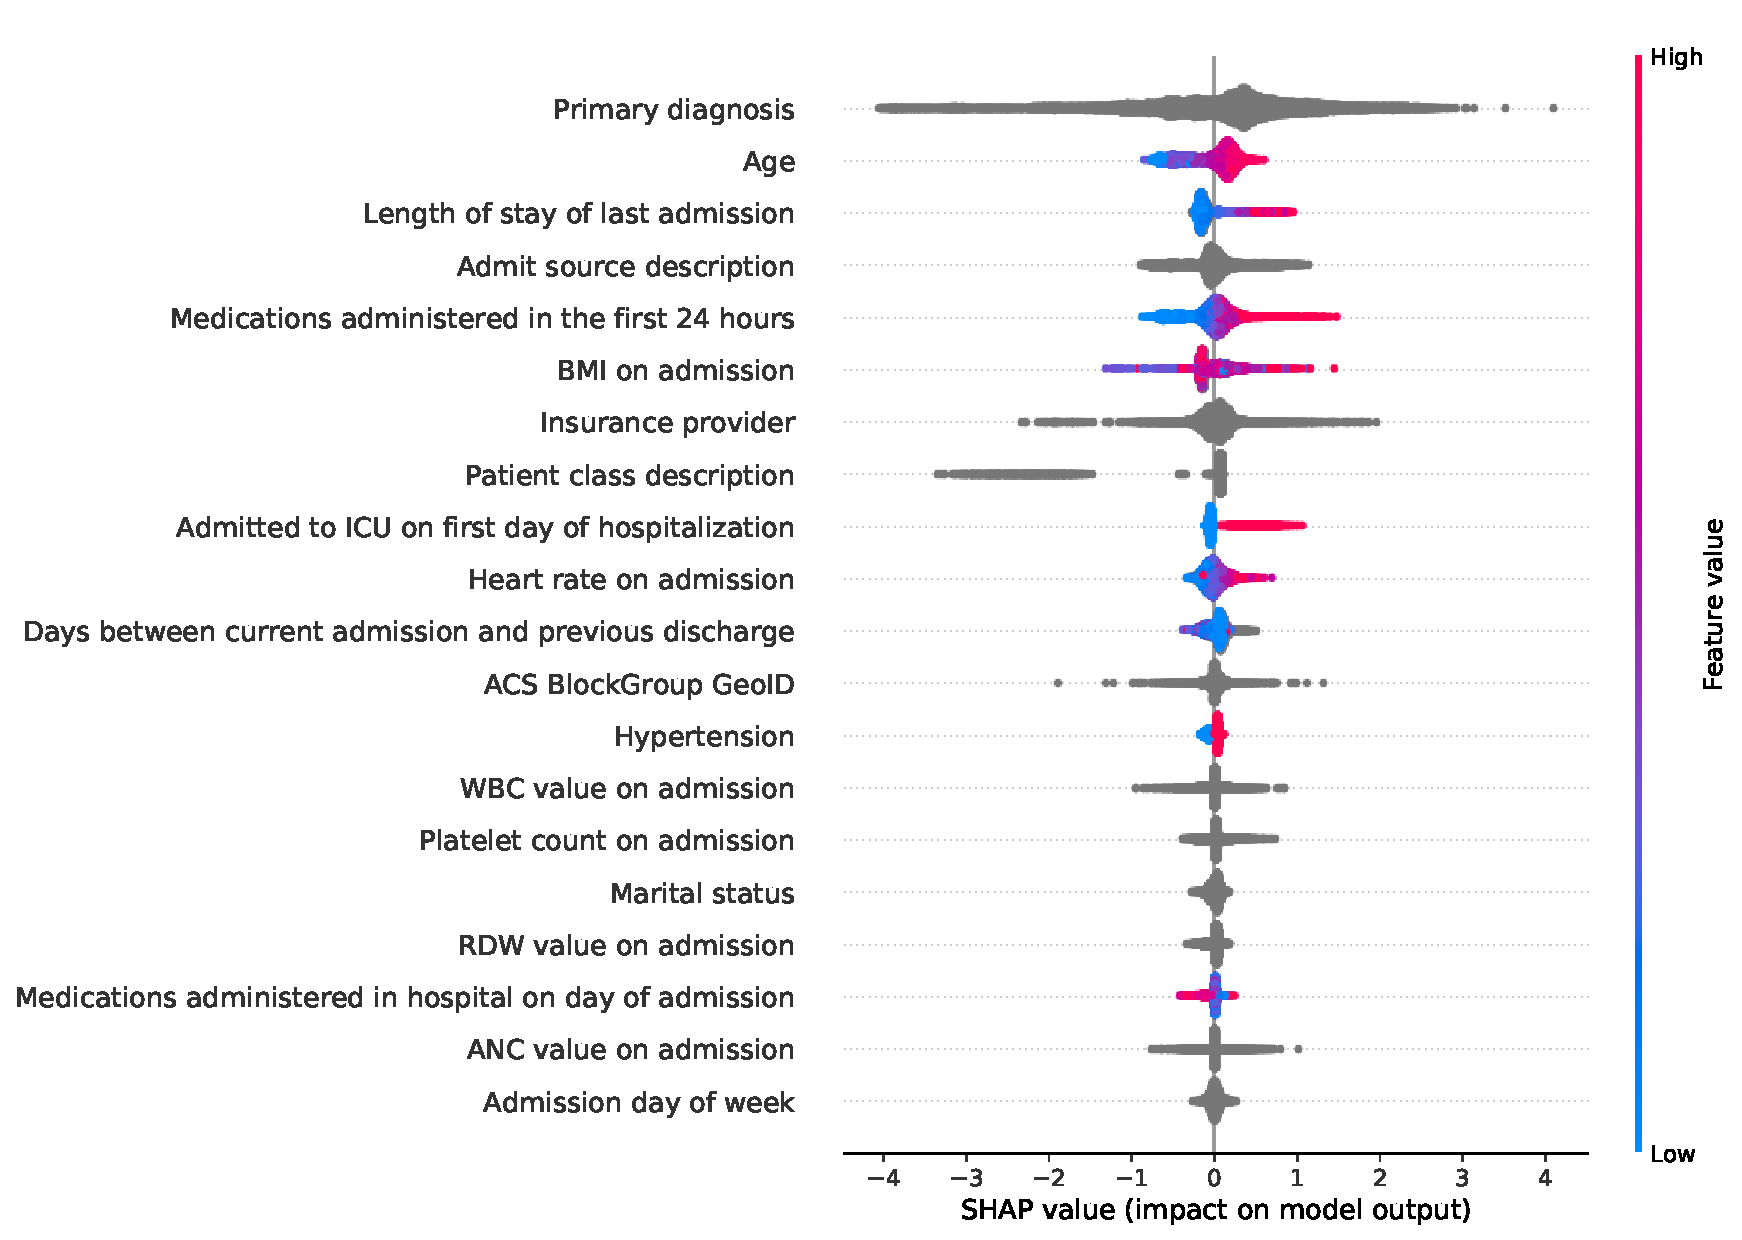
\includegraphics[width=\linewidth,keepaspectratio]{supplementary/los7d_SHAP_summary.pdf}
\end{subfigure}%

\caption{\textbf{Prediction of Hospitalization Outcomes.} \\
Panels~\ref{fig:shaprdt3d},~\ref{fig:shaprdt7d},~\ref{fig:shaplos3d}, and~\ref{fig:shaplos7d} 
show the most impactful features on prediction, 
along with the impact of high or low values for numeric features. Categorical features are shown in gray.\@
}\label{fig:suppshapfig}
\end{adjustbox}
\end{figure}
\begin{figure}
\begin{adjustbox}{minipage=7.0in,frame}
\vspace{2.5mm}
\centering

\def\picdir{supplementary/readmitted30d/}
\def\picone{readmitted30d_SHAP_dependence_2.pdf}
\def\pictwo{readmitted30d_SHAP_dependence_3.pdf}
\def\picthr{readmitted30d_SHAP_dependence_8.pdf}
\def\picfor{readmitted30d_SHAP_dependence_7.pdf}

\begin{subfigure}[t]{.45\linewidth}
    \centering
    \captionsetup[subfigure]{}
    \caption{Age vs.\ number of past hospitalizations.}\label{fig:30dintageadmits}
    \includegraphics[height=3in,width=3in,keepaspectratio]{\picdir\picone}
\end{subfigure}%
\hspace{5mm}%
\begin{subfigure}[t]{.45\linewidth}
    \centering
    \captionsetup[subfigure]{}
    \caption{Length of stay of current vs.\ past hospitalization.}\label{fig:30dintlos}
    \includegraphics[height=3in,width=3in,keepaspectratio]{\picdir\pictwo}
\end{subfigure}%

\vspace{5mm}
\begin{subfigure}[t]{.45\linewidth}
    \centering
    \captionsetup[subfigure]{}
    \caption{Heart rate vs.\ age.}\label{fig:30dinthrage}
    % \vspace{5mm}
    \includegraphics[height=2.7in,width=3in,keepaspectratio]{\picdir\picthr}
\end{subfigure}%
\hspace{5mm}%
\begin{subfigure}[t]{.45\linewidth}
    \centering
    \captionsetup[subfigure]{}
    \caption{Discharge disposition vs.\ number of past hospitalizations.}\label{fig:30dintdispoadmits}
    \includegraphics[height=2.7in,width=3in,keepaspectratio]{\picdir\picfor}
\end{subfigure}%

\caption{\textbf{Variable Interactions for 30-day Readmission.} \\
Panels~\ref{fig:30dintageadmits},~\ref{fig:30dintlos},%
~\ref{fig:30dinthrage}, and~\ref{fig:30dintdispoadmits} 
show changes in model output (SHAP values---left axis)
as an effect of the interplay between 
values of indicated variables (x-axis and color-coded points, 
color code shown on right axis).\@
Each point is a single hospitalization.\@
Gray points or values less than zero indicate missing values for the variable indicated,
e.g.\ a person who has never been hospitalized before
will have a null ``length of stay of last admission.''\@
}\label{fig:30dint}
\end{adjustbox}
\end{figure}
\begin{figure}
\begin{adjustbox}{minipage=7.0in,frame}
\vspace{2.5mm}
\centering
%
\def\picdir{supplementary/los5d/}
%
\def\labbig{fig:los5dint}
%
\def\picone{los5d_SHAP_dependence_2.pdf}
\def\pictwo{los5d_SHAP_dependence_3.pdf}
\def\picthr{los5d_SHAP_dependence_9.pdf}
\def\picfor{los5d_SHAP_dependence_9a.pdf}
% 1
\def\capone{Number of medications administered in first 24 hours vs.\ age.}
\def\labone{fig:los5dintagemeds}
% 2
\def\captwo{Length of stay of last hospitalization vs.\ days since last hospitalization.}
\def\labtwo{fig:los5dintlostimesince}
% 3
\def\capthr{Heart rate vs.\ age.}
\def\labthr{fig:los5dinthrage}
% 4
\def\capfor{ICU admission vs.\ number of medications administered in last 24 hours.}
\def\labfor{fig:los5dinticumeds}
%
\def\capbig{\textbf{Variable Interactions for Length of Stay Over 5 Days.} \\ %
Panels~\ref{\labone},~\ref{\labtwo}, %
~\ref{\labthr}, and~\ref{\labfor} %
show changes in model output (SHAP values---left axis) %
as an effect of the interplay between %
values of indicated variables (x-axis and color-coded points, %
color code shown on right axis).\@
Each point is a single hospitalization.\@
Gray points or values less than zero indicate missing values for the variable indicated,
e.g.\ a person who has never been hospitalized before %
will have a null ``length of stay of last admission.''\@
}
%
%
\begin{subfigure}[t]{.45\linewidth}
    \centering
    \captionsetup[subfigure]{}
    \caption{\capone{}}\label{\labone}
    \includegraphics[height=3in,width=3in,keepaspectratio]{\picdir\picone}
\end{subfigure}%
\hspace{5mm}%
\begin{subfigure}[t]{.45\linewidth}
    \centering
    \captionsetup[subfigure]{}
    \caption{\captwo}\label{\labtwo}
    \includegraphics[height=3in,width=3in,keepaspectratio]{\picdir\pictwo}
\end{subfigure}%

\vspace{5mm}
\begin{subfigure}[t]{.45\linewidth}
    \centering
    \captionsetup[subfigure]{}
    \caption{\capthr}\label{\labthr}
    \includegraphics[height=2.7in,width=3in,keepaspectratio]{\picdir\picthr}
\end{subfigure}%
\hspace{5mm}%
\begin{subfigure}[t]{.45\linewidth}
    \centering
    \captionsetup[subfigure]{}
    \caption{\capfor}\label{\labfor}
    \includegraphics[height=2.7in,width=3in,keepaspectratio]{\picdir\picfor}
\end{subfigure}%

\caption{\capbig}\label{\labbig}
\end{adjustbox}
\end{figure}
\begin{figure}
\begin{adjustbox}{minipage=7.0in,frame}
\vspace{2.5mm}
\centering
%
\def\target{age}
%
\def\picdir{supplementary/\target/}
%
\def\labbig{fig:ageint}
%
\def\picone{\target_SHAP_dependence_1.pdf}
\def\pictwo{\target_SHAP_dependence_2.pdf}
\def\picthr{\target_SHAP_dependence_3.pdf}
\def\picfor{\target_SHAP_dependence_5.pdf}
% 1
\def\capone{Diagnosis of hypertension vs.\ medications administered on day of discharge.}
\def\labone{fig:ageinthtnmeds}
% 2
\def\captwo{Marital status vs.\ gender.}
\def\labtwo{fig:ageintmarriagegender}
% 3
\def\capthr{Discharge disposition vs.\ number of morbidities.}
\def\labthr{fig:ageintdispomorbid}
% 4
\def\capfor{Systolic vs.\ diastolic blood pressure on discharge.}
\def\labfor{fig:ageintsysdiabp}
%
\def\capbig{\textbf{Variable Interactions for \titlecap{\target}.} \\ %
Panels~\ref{\labone},~\ref{\labtwo}, %
~\ref{\labthr}, and~\ref{\labfor} %
show changes in model output (SHAP values---left axis) %
as an effect of the interplay between %
values of indicated variables (x-axis and color-coded points, %
color code shown on right axis).\@
Each point is a single hospitalization.\@
Values less than zero indicate missing values for the variable indicated,
e.g.\ an unrecorded systolic blood pressure on discharge (\ref{\labfor})  %
will have a value less than zero.\@
}
%
%
\begin{subfigure}[t]{.45\linewidth}
    \centering
    \captionsetup[subfigure]{}
    \caption{\capone{}}\label{\labone}
    \includegraphics[height=3in,width=3in,keepaspectratio]{\picdir\picone}
\end{subfigure}%
\hspace{5mm}%
\begin{subfigure}[t]{.45\linewidth}
    \centering
    \captionsetup[subfigure]{}
    \caption{\captwo}\label{\labtwo}
    \includegraphics[height=3in,width=3in,keepaspectratio]{\picdir\pictwo}
\end{subfigure}%

\vspace{5mm}
\begin{subfigure}[t]{.45\linewidth}
    \centering
    \captionsetup[subfigure]{}
    \caption{\capthr}\label{\labthr}
    \includegraphics[height=2.7in,width=3in,keepaspectratio]{\picdir\picthr}
\end{subfigure}%
\hspace{5mm}%
\begin{subfigure}[t]{.45\linewidth}
    \centering
    \captionsetup[subfigure]{}
    \caption{\capfor}\label{\labfor}
    \includegraphics[height=2.7in,width=3in,keepaspectratio]{\picdir\picfor}
\end{subfigure}%

\caption{\capbig}\label{\labbig}
\end{adjustbox}
\end{figure}
\begin{figure}
\begin{adjustbox}{minipage=7.0in,frame}
\vspace{2.5mm}
\centering
%
\def\target{race}
%
\def\picdir{supplementary/\target/}
%
\def\labbig{fig:raceint}
%
\def\picone{\target_SHAP_dependence_8.pdf}
\def\pictwo{\target_SHAP_dependence_5.pdf}
\def\picthr{\target_SHAP_dependence_3.pdf}
\def\picfor{\target_SHAP_dependence_2.pdf}
% 1
\def\capone{Number of families with income over twice the poverty level vs.\ number of families with female householder and no husband present.}
\def\labone{fig:raceintincfemhh}
% 2
\def\captwo{Employed population count vs.\ number of married couple families.}
\def\labtwo{fig:raceintempmarried}
% 3
\def\capthr{Marital status vs.\ age.}
\def\labthr{fig:raceintmarriedage}
% 4
\def\capfor{Age vs.\ hypertension.}
\def\labfor{fig:raceintagehtn}
%
\def\capbig{\textbf{Variable Interactions for \titlecap{\target}.} \\ %
Panels~\ref{\labone},~\ref{\labtwo}, %
~\ref{\labthr}, and~\ref{\labfor} %
show changes in model output (SHAP values---left axis) %
as an effect of the interplay between %
values of indicated variables (x-axis and color-coded points, %
color code shown on right axis).\@
Each point is a single hospitalization.\@
Values less than zero or gray points indicate missing information, e.g.\ 
a patient without an available ACS BlockGroup ID 
for whom other ACS information cannot be obtained (see~\ref{\labone} and~\ref{\labtwo}).\@
}
%
%
\begin{subfigure}[t]{.45\linewidth}
    \centering
    \captionsetup[subfigure]{}
    \caption{\capone{}}\label{\labone}
    \includegraphics[height=3in,width=3in,keepaspectratio]{\picdir\picone}
\end{subfigure}%
\hspace{5mm}%
\begin{subfigure}[t]{.45\linewidth}
    \centering
    \captionsetup[subfigure]{}
    \caption{\captwo}\label{\labtwo}
    \includegraphics[height=3in,width=3in,keepaspectratio]{\picdir\pictwo}
\end{subfigure}%

\vspace{5mm}
\begin{subfigure}[t]{.45\linewidth}
    \centering
    \captionsetup[subfigure]{}
    \caption{\capthr}\label{\labthr}
    \includegraphics[height=2.7in,width=3in,keepaspectratio]{\picdir\picthr}
\end{subfigure}%
\hspace{5mm}%
\begin{subfigure}[t]{.45\linewidth}
    \centering
    \captionsetup[subfigure]{}
    \caption{\capfor}\label{\labfor}
    \includegraphics[height=2.7in,width=3in,keepaspectratio]{\picdir\picfor}
\end{subfigure}%

\caption{\capbig}\label{\labbig}
\end{adjustbox}
\end{figure}
\begin{figure}
    \begin{adjustbox}{minipage=7.0in,frame}
    \vspace{2.5mm}
    \centering
    %
    \def\target{gender}
    %
    \def\picdir{supplementary/\target/}
    %
    \def\labbig{fig:genderint}
    %
    \def\picone{\target_SHAP_dependence_1.pdf}
    \def\pictwo{\target_SHAP_dependence_6.pdf}
    \def\picthr{\target_SHAP_dependence_7.pdf}
    \def\picfor{\target_SHAP_dependence_9.pdf}
    % 1
    \def\capone{Marital status vs.\ age.}
    \def\labone{fig:genderintmarriedage}
    % 2
    \def\captwo{Age vs.\ marital status}
    \def\labtwo{fig:genderintagemarried}
    % 3
    \def\capthr{Diastolic blood pressure vs.\ medications administered on day of admission.}
    \def\labthr{fig:genderintdbpmeds}
    % 4
    \def\capfor{Diagnosis of anxiety vs.\ age.}
    \def\labfor{fig:genderintanxietyage}
    %
    \def\capbig{\textbf{Variable Interactions for \titlecap{\target}.} \\ %
    Panels~\ref{\labone},~\ref{\labtwo},%
    ~\ref{\labthr}, and~\ref{\labfor} % 
    show changes in model output (SHAP values---left axis) %
    as an effect of the interplay between %
    values of indicated variables (x-axis and color-coded points, %
    color code shown on right axis).\@
    Each point is a single hospitalization.\@
    Values less than zero indicate missing values for the variable indicated, %
    e.g.\ a person for whom admission diastolic blood pressure was not available in the chart (\ref{\labthr}).\@
    }
    %
    %
    \begin{subfigure}[t]{.45\linewidth}
        \centering
        \captionsetup[subfigure]{}
        \caption{\capone{}}\label{\labone}
        \includegraphics[height=3in,width=3in,keepaspectratio]{\picdir\picone}
    \end{subfigure}%
    \hspace{5mm}%
    \begin{subfigure}[t]{.45\linewidth}
        \centering
        \captionsetup[subfigure]{}
        \caption{\captwo}\label{\labtwo}
        \includegraphics[height=3in,width=3in,keepaspectratio]{\picdir\pictwo}
    \end{subfigure}%
    
    \vspace{5mm}
    \begin{subfigure}[t]{.45\linewidth}
        \centering
        \captionsetup[subfigure]{}
        \caption{\capthr}\label{\labthr}
        \includegraphics[height=2.7in,width=3in,keepaspectratio]{\picdir\picthr}
    \end{subfigure}%
    \hspace{5mm}%
    \begin{subfigure}[t]{.45\linewidth}
        \centering
        \captionsetup[subfigure]{}
        \caption{\capfor}\label{\labfor}
        \includegraphics[height=2.7in,width=3in,keepaspectratio]{\picdir\picfor}
    \end{subfigure}%
    
    \caption{\capbig}\label{\labbig}
    \end{adjustbox}
    \end{figure}
\begin{figure}
\begin{adjustbox}{minipage=7.0in,frame}
\vspace{2.5mm}
\centering
%
\def\target{financialclass}
\def\targetname{Financial Class}
%
\def\picdir{supplementary/\target/}
%
\def\labbig{fig:insuranceint}
%
\def\picone{\target_SHAP_dependence_0.pdf}
\def\pictwo{\target_SHAP_dependence_1.pdf}
\def\picthr{\target_SHAP_dependence_5.pdf}
\def\picfor{\target_SHAP_dependence_7.pdf}
% 1
\def\capone{Age vs.\ race.}
\def\labone{fig:insuranceintagerace}
% 2
\def\captwo{Marital status vs.\ age.}
\def\labtwo{fig:insuranceintmarriedage}
% 3
\def\capthr{Hypertension vs.\ race.}
\def\labthr{fig:insuranceinthtnrace}
% 4
\def\capfor{Number of emergency department visits vs.\ age.}
\def\labfor{fig:insuranceintedage}
%
\def\capbig{\textbf{Variable Interactions for \titlecap{\targetname}.} \\ %
Panels~\ref{\labone},~\ref{\labtwo}, %
~\ref{\labthr}, and~\ref{\labfor} %
show changes in model output (SHAP values---left axis) %
as an effect of the interplay between %
values of indicated variables (x-axis and color-coded points, %
color code shown on right axis).\@
Each point is a single hospitalization.\@
}
%
%
\begin{subfigure}[t]{.45\linewidth}
    \centering
    \captionsetup[subfigure]{}
    \caption{\capone{}}\label{\labone}
    \includegraphics[height=3in,width=3in,keepaspectratio]{\picdir\picone}
\end{subfigure}%
\hspace{5mm}%
\begin{subfigure}[t]{.45\linewidth}
    \centering
    \captionsetup[subfigure]{}
    \caption{\captwo}\label{\labtwo}
    \includegraphics[height=3in,width=3in,keepaspectratio]{\picdir\pictwo}
\end{subfigure}%

\vspace{5mm}
\begin{subfigure}[t]{.45\linewidth}
    \centering
    \captionsetup[subfigure]{}
    \caption{\capthr}\label{\labthr}
    \includegraphics[height=2.7in,width=3in,keepaspectratio]{\picdir\picthr}
\end{subfigure}%
\hspace{5mm}%
\begin{subfigure}[t]{.45\linewidth}
    \centering
    \captionsetup[subfigure]{}
    \caption{\capfor}\label{\labfor}
    \includegraphics[height=2.7in,width=3in,keepaspectratio]{\picdir\picfor}
\end{subfigure}%

\caption{\capbig}\label{\labbig}
\end{adjustbox}
\end{figure}
%
% TODO:
% Tables
% \rowcolors{3}{}{NEJMAlternatingRows} 
\begin{adjustbox}{width={\textwidth},keepaspectratio,frame}%
{
\begin{tabular}{lcccc}
\rowcolor{NEJMTopRow} \multicolumn{2}{l}
{{\textbf{\color{NEJMRed} Table 2.}}
\textbf{Variables Included in Prediction of Length of Stay Over 5 Days}} 
\\
\hline
\textbf{Target} & \textbf{ROC AUC} & \textbf{Brier Score Loss} &   \textbf{RMSE} \\
                        %   &         &                  &                   &        \\
Readmitted within 30 days &    0.76 &              0.10 &        -- \\
Readmitted within 7 days  &    0.70 &              0.04 &        -- \\
Readmitted within 5 days  &    0.69 &              0.03 &        -- \\
Readmitted within 3 days  &    0.65 &              0.02 &        -- \\
Days to readmission       &      -- &                -- &      8.98 \\
Hospital stay over 7 days &    0.85 &              0.12 &        -- \\
Hospital stay over 5 days &    0.85 &              0.14 &        -- \\
Hospital stay over 3 days &    0.86 &              0.15 &        -- \\
Length of stay (days)     &      -- &                -- &      3.94 \\
Gender                    &    0.87 &              0.14 &        -- \\
Race                      &    0.91 &              0.10 &        -- \\
Financial Class           &    0.92 &              0.10 &        -- \\
Age over 65 years         &    0.94 &              0.09 &        -- \\
Age (years)               &      -- &                -- &     10.37 \\
\end{tabular}
\label{table:tablelos}
}
\end{adjustbox}%
\end{document}%